
%% bare_jrnl_compsoc.tex
%% V1.4b
%% 2015/08/26
%% by Michael Shell
%% See:
%% http://www.michaelshell.org/
%% for current contact information.
%%
%% This is a skeleton file demonstrating the use of IEEEtran.cls
%% (requires IEEEtran.cls version 1.8b or later) with an IEEE
%% Computer Society journal paper.
%%
%% Support sites:
%% http://www.michaelshell.org/tex/ieeetran/
%% http://www.ctan.org/pkg/ieeetran
%% and
%% http://www.ieee.org/

%%*************************************************************************
%% Legal Notice:
%% This code is offered as-is without any warranty either expressed or
%% implied; without even the implied warranty of MERCHANTABILITY or
%% FITNESS FOR A PARTICULAR PURPOSE!
%% User assumes all risk.
%% In no event shall the IEEE or any contributor to this code be liable for
%% any damages or losses, including, but not limited to, incidental,
%% consequential, or any other damages, resulting from the use or misuse
%% of any information contained here.
%%
%% All comments are the opinions of their respective authors and are not
%% necessarily endorsed by the IEEE.
%%
%% This work is distributed under the LaTeX Project Public License (LPPL)
%% ( http://www.latex-project.org/ ) version 1.3, and may be freely used,
%% distributed and modified. A copy of the LPPL, version 1.3, is included
%% in the base LaTeX documentation of all distributions of LaTeX released
%% 2003/12/01 or later.
%% Retain all contribution notices and credits.
%% ** Modified files should be clearly indicated as such, including  **
%% ** renaming them and changing author support contact information. **
%%*************************************************************************


% *** Authors should verify (and, if needed, correct) their LaTeX system  ***
% *** with the testflow diagnostic prior to trusting their LaTeX platform ***
% *** with production work. The IEEE's font choices and paper sizes can   ***
% *** trigger bugs that do not appear when using other class files.       ***                          ***
% The testflow support page is at:
% http://www.michaelshell.org/tex/testflow/


\documentclass[conference]{IEEEtran}
%
% If IEEEtran.cls has not been installed into the LaTeX system files,
% manually specify the path to it like:
% \documentclass[10pt,journal,compsoc]{../sty/IEEEtran}





% Some very useful LaTeX packages include:
% (uncomment the ones you want to load)


% *** MISC UTILITY PACKAGES ***
%
%\usepackage{ifpdf}
% Heiko Oberdiek's ifpdf.sty is very useful if you need conditional
% compilation based on whether the output is pdf or dvi.
% usage:
% \ifpdf
%   % pdf code
% \else
%   % dvi code
% \fi
% The latest version of ifpdf.sty can be obtained from:
% http://www.ctan.org/pkg/ifpdf
% Also, note that IEEEtran.cls V1.7 and later provides a builtin
% \ifCLASSINFOpdf conditional that works the same way.
% When switching from latex to pdflatex and vice-versa, the compiler may
% have to be run twice to clear warning/error messages.






% *** CITATION PACKAGES ***
%
\ifCLASSOPTIONcompsoc
  % IEEE Computer Society needs nocompress option
  % requires cite.sty v4.0 or later (November 2003)
  \usepackage[nocompress]{cite}
\else
  % normal IEEE
  \usepackage{cite}
\fi
% cite.sty was written by Donald Arseneau
% V1.6 and later of IEEEtran pre-defines the format of the cite.sty package
% \cite{} output to follow that of the IEEE. Loading the cite package will
% result in citation numbers being automatically sorted and properly
% "compressed/ranged". e.g., [1], [9], [2], [7], [5], [6] without using
% cite.sty will become [1], [2], [5]--[7], [9] using cite.sty. cite.sty's
% \cite will automatically add leading space, if needed. Use cite.sty's
% noadjust option (cite.sty V3.8 and later) if you want to turn this off
% such as if a citation ever needs to be enclosed in parenthesis.
% cite.sty is already installed on most LaTeX systems. Be sure and use
% version 5.0 (2009-03-20) and later if using hyperref.sty.
% The latest version can be obtained at:
% http://www.ctan.org/pkg/cite
% The documentation is contained in the cite.sty file itself.
%
% Note that some packages require special options to format as the Computer
% Society requires. In particular, Computer Society  papers do not use
% compressed citation ranges as is done in typical IEEE papers
% (e.g., [1]-[4]). Instead, they list every citation separately in order
% (e.g., [1], [2], [3], [4]). To get the latter we need to load the cite
% package with the nocompress option which is supported by cite.sty v4.0
% and later. Note also the use of a CLASSOPTION conditional provided by
% IEEEtran.cls V1.7 and later.





% *** GRAPHICS RELATED PACKAGES ***
%
\ifCLASSINFOpdf
  % \usepackage[pdftex]{graphicx}
  % declare the path(s) where your graphic files are
  % \graphicspath{{../pdf/}{../jpeg/}}
  % and their extensions so you won't have to specify these with
  % every instance of \includegraphics
  % \DeclareGraphicsExtensions{.pdf,.jpeg,.png}
\else
  % or other class option (dvipsone, dvipdf, if not using dvips). graphicx
  % will default to the driver specified in the system graphics.cfg if no
  % driver is specified.
  % \usepackage[dvips]{graphicx}
  % declare the path(s) where your graphic files are
  % \graphicspath{{../eps/}}
  % and their extensions so you won't have to specify these with
  % every instance of \includegraphics
  % \DeclareGraphicsExtensions{.eps}
\fi
% graphicx was written by David Carlisle and Sebastian Rahtz. It is
% required if you want graphics, photos, etc. graphicx.sty is already
% installed on most LaTeX systems. The latest version and documentation
% can be obtained at:
% http://www.ctan.org/pkg/graphicx
% Another good source of documentation is "Using Imported Graphics in
% LaTeX2e" by Keith Reckdahl which can be found at:
% http://www.ctan.org/pkg/epslatex
%
% latex, and pdflatex in dvi mode, support graphics in encapsulated
% postscript (.eps) format. pdflatex in pdf mode supports graphics
% in .pdf, .jpeg, .png and .mps (metapost) formats. Users should ensure
% that all non-photo figures use a vector format (.eps, .pdf, .mps) and
% not a bitmapped formats (.jpeg, .png). The IEEE frowns on bitmapped formats
% which can result in "jaggedy"/blurry rendering of lines and letters as
% well as large increases in file sizes.
%
% You can find documentation about the pdfTeX application at:
% http://www.tug.org/applications/pdftex






% *** MATH PACKAGES ***
%
%\usepackage{amsmath}
% A popular package from the American Mathematical Society that provides
% many useful and powerful commands for dealing with mathematics.
%
% Note that the amsmath package sets \interdisplaylinepenalty to 10000
% thus preventing page breaks from occurring within multiline equations. Use:
%\interdisplaylinepenalty=2500
% after loading amsmath to restore such page breaks as IEEEtran.cls normally
% does. amsmath.sty is already installed on most LaTeX systems. The latest
% version and documentation can be obtained at:
% http://www.ctan.org/pkg/amsmath





% *** SPECIALIZED LIST PACKAGES ***
%
%\usepackage{algorithmic}
% algorithmic.sty was written by Peter Williams and Rogerio Brito.
% This package provides an algorithmic environment fo describing algorithms.
% You can use the algorithmic environment in-text or within a figure
% environment to provide for a floating algorithm. Do NOT use the algorithm
% floating environment provided by algorithm.sty (by the same authors) or
% algorithm2e.sty (by Christophe Fiorio) as the IEEE does not use dedicated
% algorithm float types and packages that provide these will not provide
% correct IEEE style captions. The latest version and documentation of
% algorithmic.sty can be obtained at:
% http://www.ctan.org/pkg/algorithms
% Also of interest may be the (relatively newer and more customizable)
% algorithmicx.sty package by Szasz Janos:
% http://www.ctan.org/pkg/algorithmicx




% *** ALIGNMENT PACKAGES ***
%
%\usepackage{array}
% Frank Mittelbach's and David Carlisle's array.sty patches and improves
% the standard LaTeX2e array and tabular environments to provide better
% appearance and additional user controls. As the default LaTeX2e table
% generation code is lacking to the point of almost being broken with
% respect to the quality of the end results, all users are strongly
% advised to use an enhanced (at the very least that provided by array.sty)
% set of table tools. array.sty is already installed on most systems. The
% latest version and documentation can be obtained at:
% http://www.ctan.org/pkg/array


% IEEEtran contains the IEEEeqnarray family of commands that can be used to
% generate multiline equations as well as matrices, tables, etc., of high
% quality.




% *** SUBFIGURE PACKAGES ***
%\ifCLASSOPTIONcompsoc
%  \usepackage[caption=false,font=footnotesize,labelfont=sf,textfont=sf]{subfig}
%\else
%  \usepackage[caption=false,font=footnotesize]{subfig}
%\fi
% subfig.sty, written by Steven Douglas Cochran, is the modern replacement
% for subfigure.sty, the latter of which is no longer maintained and is
% incompatible with some LaTeX packages including fixltx2e. However,
% subfig.sty requires and automatically loads Axel Sommerfeldt's caption.sty
% which will override IEEEtran.cls' handling of captions and this will result
% in non-IEEE style figure/table captions. To prevent this problem, be sure
% and invoke subfig.sty's "caption=false" package option (available since
% subfig.sty version 1.3, 2005/06/28) as this is will preserve IEEEtran.cls
% handling of captions.
% Note that the Computer Society format requires a sans serif font rather
% than the serif font used in traditional IEEE formatting and thus the need
% to invoke different subfig.sty package options depending on whether
% compsoc mode has been enabled.
%
% The latest version and documentation of subfig.sty can be obtained at:
% http://www.ctan.org/pkg/subfig




% *** FLOAT PACKAGES ***
%
%\usepackage{fixltx2e}
% fixltx2e, the successor to the earlier fix2col.sty, was written by
% Frank Mittelbach and David Carlisle. This package corrects a few problems
% in the LaTeX2e kernel, the most notable of which is that in current
% LaTeX2e releases, the ordering of single and double column floats is not
% guaranteed to be preserved. Thus, an unpatched LaTeX2e can allow a
% single column figure to be placed prior to an earlier double column
% figure.
% Be aware that LaTeX2e kernels dated 2015 and later have fixltx2e.sty's
% corrections already built into the system in which case a warning will
% be issued if an attempt is made to load fixltx2e.sty as it is no longer
% needed.
% The latest version and documentation can be found at:
% http://www.ctan.org/pkg/fixltx2e


%\usepackage{stfloats}
% stfloats.sty was written by Sigitas Tolusis. This package gives LaTeX2e
% the ability to do double column floats at the bottom of the page as well
% as the top. (e.g., "\begin{figure*}[!b]" is not normally possible in
% LaTeX2e). It also provides a command:
%\fnbelowfloat
% to enable the placement of footnotes below bottom floats (the standard
% LaTeX2e kernel puts them above bottom floats). This is an invasive package
% which rewrites many portions of the LaTeX2e float routines. It may not work
% with other packages that modify the LaTeX2e float routines. The latest
% version and documentation can be obtained at:
% http://www.ctan.org/pkg/stfloats
% Do not use the stfloats baselinefloat ability as the IEEE does not allow
% \baselineskip to stretch. Authors submitting work to the IEEE should note
% that the IEEE rarely uses double column equations and that authors should try
% to avoid such use. Do not be tempted to use the cuted.sty or midfloat.sty
% packages (also by Sigitas Tolusis) as the IEEE does not format its papers in
% such ways.
% Do not attempt to use stfloats with fixltx2e as they are incompatible.
% Instead, use Morten Hogholm'a dblfloatfix which combines the features
% of both fixltx2e and stfloats:
%
% \usepackage{dblfloatfix}
% The latest version can be found at:
% http://www.ctan.org/pkg/dblfloatfix




%\ifCLASSOPTIONcaptionsoff
%  \usepackage[nomarkers]{endfloat}
% \let\MYoriglatexcaption\caption
% \renewcommand{\caption}[2][\relax]{\MYoriglatexcaption[#2]{#2}}
%\fi
% endfloat.sty was written by James Darrell McCauley, Jeff Goldberg and
% Axel Sommerfeldt. This package may be useful when used in conjunction with
% IEEEtran.cls'  captionsoff option. Some IEEE journals/societies require that
% submissions have lists of figures/tables at the end of the paper and that
% figures/tables without any captions are placed on a page by themselves at
% the end of the document. If needed, the draftcls IEEEtran class option or
% \CLASSINPUTbaselinestretch interface can be used to increase the line
% spacing as well. Be sure and use the nomarkers option of endfloat to
% prevent endfloat from "marking" where the figures would have been placed
% in the text. The two hack lines of code above are a slight modification of
% that suggested by in the endfloat docs (section 8.4.1) to ensure that
% the full captions always appear in the list of figures/tables - even if
% the user used the short optional argument of \caption[]{}.
% IEEE papers do not typically make use of \caption[]'s optional argument,
% so this should not be an issue. A similar trick can be used to disable
% captions of packages such as subfig.sty that lack options to turn off
% the subcaptions:
% For subfig.sty:
% \let\MYorigsubfloat\subfloat
% \renewcommand{\subfloat}[2][\relax]{\MYorigsubfloat[]{#2}}
% However, the above trick will not work if both optional arguments of
% the \subfloat command are used. Furthermore, there needs to be a
% description of each subfigure *somewhere* and endfloat does not add
% subfigure captions to its list of figures. Thus, the best approach is to
% avoid the use of subfigure captions (many IEEE journals avoid them anyway)
% and instead reference/explain all the subfigures within the main caption.
% The latest version of endfloat.sty and its documentation can obtained at:
% http://www.ctan.org/pkg/endfloat
%
% The IEEEtran \ifCLASSOPTIONcaptionsoff conditional can also be used
% later in the document, say, to conditionally put the References on a
% page by themselves.




% *** PDF, URL AND HYPERLINK PACKAGES ***
%
%\usepackage{url}
% url.sty was written by Donald Arseneau. It provides better support for
% handling and breaking URLs. url.sty is already installed on most LaTeX
% systems. The latest version and documentation can be obtained at:
% http://www.ctan.org/pkg/url
% Basically, \url{my_url_here}.





% *** Do not adjust lengths that control margins, column widths, etc. ***
% *** Do not use packages that alter fonts (such as pslatex).         ***
% There should be no need to do such things with IEEEtran.cls V1.6 and later.
% (Unless specifically asked to do so by the journal or conference you plan
% to submit to, of course. )


% correct bad hyphenation here
\hyphenation{op-tical net-works semi-conduc-tor}

\usepackage{balance}  % to better equalize the last page
\usepackage{graphics} % for EPS, load graphicx instead
%\usepackage[T1]{fontenc}
\usepackage{txfonts}
\usepackage{times}    % comment if you want LaTeX's default font
\usepackage[pdftex]{hyperref}
% \usepackage{url}      % llt: nicely formatted URLs
\usepackage{color}
\usepackage{textcomp}
\usepackage{booktabs}
\usepackage{ccicons}


\usepackage{cite}
\usepackage{url}
\usepackage{fancybox}
\usepackage{multirow}
\usepackage{flushend}
\usepackage{booktabs}
\usepackage{tabularx}
\usepackage{comment}
\usepackage{array}
\usepackage[flushleft]{threeparttable}
\usepackage{mdframed}
\graphicspath{{}{images/}{dia/}}
\DeclareGraphicsExtensions{.pdf,.png}


\usepackage{listings}
\usepackage{courier}
\usepackage{hyperref}

\usepackage{xpatch}
\xdef\scr{}

\xpatchcmd{\refstepcounter}{%
  \stepcounter{#1}%
}{%
  \stepcounter{#1}%
  \xdef\scr{\number\value{#1}}%
}{\typeout{success}}{\typeout{failure}}


\newcounter{o}
\setcounter{o}{0}
\usepackage{soul}
\usepackage{tikz}
%colors
\definecolor{1c1}{RGB}{188,162,6}
\definecolor{1c2}{RGB}{137,129,80}
\definecolor{1c3}{RGB}{239,167,31}
\definecolor{1c4}{RGB}{88,194,241}
\definecolor{1c5}{RGB}{6,180,188}

% stiles used
\tikzset{mynode/.style={draw=white,solid,circle,fill=green,inner sep=1pt, thick,
text=black}}
%draw=black to get a black circle, fill=white so it actually has a
%background and text=black to not get that rendered in the specified color
\tikzset{arrow line/.style={dashed, line width= 2.5pt, color=#1}}

\def\bf{\textbf}
\def\eq {Equation~}
\def\eqm {Eq~}
\def\eqs {Equations~}
\def\fig {Figure~}
\def\figs {Figures~}
\def\tbl {Table~}
\def\tbls {Tables~}
\def\ie{\textit{i.e.,}}
\def\eg{\textit{e.g.,}}
\def\sec {Section~}
\def\secs {Sections~}
\def\alg {Algorithm~}
\def\algs {Algorithms~}
\def\app {Appendix~}
\def\it{\textit}
\def\tr{\textrm}
\def\tt{\mct}
\newcommand{\ib}[1]{{\textbf {\textit { #1}}}}
\newcommand{\ts}[1]{{\textsc {{ #1}}}}
\newcommand{\mct}[1]{{\footnotesize {\texttt {#1}}}}
\newcommand{\Foutse}[1]{\textcolor{red}{{\it [Foutse says: #1]}}}
\newcommand{\qu}[1]{{\it{``#1''}}}
\newcommand{\api}[1]{{\sf{\texttt\small{#1}}}}
\newcommand{\callout}[1]{{\vspace{1mm}\noindent{\fbox{\parbox{0.97\columnwidth}{#1}}}\vspace{1mm}}}
\usepackage{paralist}

\let\labelindent\relax

\newcommand{\nd}{\vspace{1mm}\noindent}
\usepackage[small,bf]{caption}
%\usepackage[toc,page]{appendix}
\usepackage{tikz}
\newcommand*\circled[1]{\tikz[baseline=(char.base)]{
            \node[shape=circle,draw,inner sep=1pt] (char) {#1};}}

 \lstset{
         language=Java,
         basicstyle=\scriptsize\ttfamily, % Standardschrift
         %numbers=left,               % Ort der Zeilennummern
         numberstyle=\tiny,          % Stil der Zeilennummern
         %stepnumber=2,               % Abstand zwischen den Zeilennummern
         numbersep=5pt,              % Abstand der Nummern zum Text
         tabsize=2,                  % Groesse von Tabs
        % extendedchars=true,         %
         breaklines=true,            % Zeilen werden Umgebrochen
%         keywordstyle=\color{black},
 %   	 frame=single,
 %        keywordstyle=[1]\textbf,    % Stil der Keywords
 %        keywordstyle=[2]\textbf,    %
 %        keywordstyle=[3]\textbf,    %
 %        keywordstyle=[4]\textbf,   \sqrt{\sqrt{}} %
         stringstyle=\color{white}\ttfamily, % Farbe der String
         showspaces=false,           % Leerzeichen anzeigen ?
         showtabs=false,             % Tabs anzeigen ?
         xleftmargin=17pt,
         framexleftmargin=17pt,
         framexrightmargin=5pt,
         framexbottommargin=4pt,
         %backgroundcolor=\color{lightgray},
         showstringspaces=false,      % Leerzeichen in Strings anzeigen ?
     %    escapeinside={\%*}{*)}
 }

\lstdefinestyle{inlinecode}{basicstyle={\ttfamily\scriptsize\bfseries}}
\newcommand\code{\lstinline[style=inlinecode]}
\newcommand{\urls}[1]{{\scriptsize\url{#1}}}
\usepackage{tcolorbox}
\newcommand{\emt}[1]{\emph{``#1''}}
\newcommand{\rev}[1]{\textcolor{blue}{#1}}

\newcommand{\gias}[1]{\textcolor{red}{{[Gias: #1]}}}
\newcommand{\dq}[1]{\href{https://stackoverflow.com/questions/#1/}{$Q_{#1}$}}
\newcommand{\da}[1]{\href{https://stackoverflow.com/answers/#1/}{$A_{#1}$}}

\usepackage{paralist}
\usepackage[outercaption]{sidecap}
\usepackage [autostyle, english = american]{csquotes}
\MakeOuterQuote{"}
\newcounter{scn}
\setcounter{scn}{1}
\usepackage[shortlabels]{enumitem}
\usepackage{tikz}
\usepackage{styles/pgf-pie}
%\usepackage{pgf-pie}
\usetikzlibrary{positioning,shadows}
\usepackage{balance}

\newif\ifpienumberinlegend
\pgfkeys{/number in legend/.code=
    \expandafter\let\expandafter\ifpienumberinlegend
    \csname if#1\endcsname
    \ifpienumberinlegend
    \let\legendbeforenumber\beforenumber
    \let\legendafternumber\afternumber
    \def\beforenumber##1\afternumber{}%
    \fi,
    /number in legend/.default=true
}
%colors
\definecolor{1c1}{RGB}{188,162,6}
\definecolor{1c2}{RGB}{137,129,80}
\definecolor{1c3}{RGB}{239,167,31}
\definecolor{1c4}{RGB}{88,194,241}
\definecolor{1c5}{RGB}{6,180,188}

% stiles used
\tikzset{mynode/.style={draw=white,solid,circle,fill=green,inner sep=1pt, thick,
text=black}}
%draw=black to get a black circle, fill=white so it actually has a
%background and text=black to not get that rendered in the specified color
\tikzset{arrow line/.style={dashed, line width= 2.5pt, color=#1}}

\usepackage{bchart}

\usepackage{xcolor}
\definecolor{ao(english)}{rgb}{0.0, 0.5, 0.0}

\newcommand{\fourbars}[4]{
{\color{red}\rule{#1pt}{6pt}}
{\color{yellow}\rule{#2pt}{6pt}}
{\color{ao(english)}\rule{#3pt}{6pt}}
{\color{cyan}\rule{#4pt}{6pt}}
}

% \newcommand{\fivebars}[5]{
% {\color{black}\rule{#1pt}{6pt}}
% {\color{yellow}\rule{#2pt}{6pt}}
% {\color{ao(english)}\rule{#3pt}{6pt}}
% {\color{cyan}\rule{#4pt}{6pt}}
% {\color{red}\rule{#5pt}{6pt}}
% }

% \newcommand{\fivebars}[5]{
% {\if#1>0 \color{black}\rule{#1pt}{6pt}#1\fi}
% {\if#2>0 \color{yellow}\rule{#2pt}{6pt}#2\fi}
% {\if#3>0 \color{ao(english)}\rule{#3pt}{6pt}#3\fi}
% {\if#4>0 \color{cyan}\rule{#4pt}{6pt}#4\fi}
% {\if#5>0 \color{red}\rule{#5pt}{6pt}#5\fi}
% }
\def\test#1{%
\ifnum0#1>0
      #1
    \fi
}
\newcommand{\fivebars}[5]{
{{\color{black}\rule{#1pt}{4pt}} \test{#1}}
{{\color{ao(english)}\rule{#2pt}{4pt}} \test{#2}}
{{\color{magenta}\rule{#3pt}{4pt}} \test{#3}}
{{\color{cyan}\rule{#4pt}{4pt}} \test{#4}}
{{\color{red}\rule{#5pt}{4pt}} \test{#5}}
}

\newcommand{\sixbars}[6]{
{{\color{black}\rule{#1pt}{4pt}} \test{#1}}
{{\color{ao(english)}\rule{#2pt}{4pt}} \test{#2}}
{{\color{magenta}\rule{#3pt}{4pt}} \test{#3}}
{{\color{red}\rule{#5pt}{4pt}} \test{#4}}
{{\color{cyan}\rule{#4pt}{4pt}} \test{#5}}
{{\color{orange}\rule{#4pt}{4pt}} \test{#6}}
}

% \newcommand{\fivebars}[5]{
% {#1\color{black}\rule{#1pt}{6pt}}
% {#2\color{yellow}\rule{#2pt}{6pt}}
% {#3\color{ao(english)}\rule{#3pt}{6pt}}
% {#4\color{cyan}\rule{#4pt}{6pt}}
% {#5\color{red}\rule{#5pt}{6pt}}
% }

\begin{document}
\title{An Empirical Study of Developer Discussions on Low Code Software Development Challenges}
\author{}% <-this % stops a
% space



\IEEEtitleabstractindextext{%
\begin{abstract}

Low code software development  (LCSD) is an emerging paradigm that combines
minimal source code with interactive graphical interfaces to promote rapid
application development. LCSD aims to democratize application development to
software practitioners with diverse backgrounds. Given that LCSD is relatively a new
paradigm, it is vital to learn about the challenges developers face during
their adoption of LCSD platforms. The online developer forum, Stack Overflow
(SO) is popular among software developers to ask for solutions to their technical
problems. We observe a growing body of posts in SO with discussions of LCSD
platforms. In this paper, we present an empirical study of around 5K SO posts
(questions + accepted answers) that contain discussions of nine popular LCSD
platforms. We apply topic modeling on the posts to determine the types of topics
discussed. We find 13 topics related to LCSD in SO. The 13 topics are grouped
into four categories: Customization, Platform Adoption, Database Management, and
Third-Party Integration. More than 40\% of the questions are about
customization, i.e., developers frequently face challenges with customising user interfaces or services offered by LCSD platforms. The
topic `Dynamic Event Handling' under the `Customization' category is the most
popular (in terms of average view counts per question of the topic) as well as
the most difficult. It means that developers frequently search for customization solutions such as how to attach dynamic events to a form in low code UI, yet most (75.9\%) of their
questions remain without an accepted answer. We manually label 900  questions
from the posts to determine the prevalence of the topics' challenges across LCSD phases. We find that most of the questions are related to the development phase, and low-code developers also face challenges with the automated testing. 
Our study findings offer implications for low-code practitioners,
platform providers, educators, and researchers.
\end{abstract}


\begin{IEEEkeywords}
Low Code, Issue, Challenge, Empirical Study.
\end{IEEEkeywords}}

%
%\ccsdesc[500]{Software and its engineering~Software libraries and repositories}
%\ccsdesc[300]{Computer systems organization~Redundancy}
%\ccsdesc{Computer systems organization~Robotics}
%\ccsdesc[100]{Networks~Network reliability}


%\keywords{API, Usage Scenario, Crowd-Sourced API Documentation, Summarization}


\maketitle



\IEEEdisplaynontitleabstractindextext
% \IEEEdisplaynontitleabstractindextext has no effect when using
% compsoc or transmag under a non-conference mode.



% For peer review papers, you can put extra information on the cover
% page as needed:
% \ifCLASSOPTIONpeerreview
% \begin{center} \bfseries EDICS Category: 3-BBND \end{center}
% \fi
%
% For peerreview papers, this IEEEtran command inserts a page break and
% creates the second title. It will be ignored for other modes.
\IEEEpeerreviewmaketitle

\section{Introduction}
LCSD is a new paradigm that enables the development of
software applications with minimal hand-coding using visual programming with
graphical interface and model-driven design. LCSD embodies End User Software Programming~\cite{Pane-MoreNatureEUSE-Springer2006} by 
democratizing application development to software practitioners from diverse backgrounds~\cite{di2020democratizing}.  
By facilitating automatic code
generation, the low-code development tools allow to develop production-ready applications with minimal coding. It
addresses the gap between domain requirement and developers' understanding that
is a common cause of delayed development in many applications with complex
business logic. The benefits of using  LCSD platforms
also include flexibility and agility, fast development time allowing
quick response to market demands, reduced bug-fixing, lower deployment effort,
and easier maintenance. Hence, the industry of low-code development is gaining
popularity at a rapid pace. According to Forrester
report~\cite{rymer2019forrester}, the  LCSD platform market is expected to be \$21 Billon by
2022. According to Gartner report by 2024 around 65\% of
large enterprises will use  LCSD platforms to some extent~\cite{wong2019low}.

To date, there are more than 200  LCSD platforms, offered by almost all major companies like Google, Saleforce~\cite{vincent2019magic}. 
Naturally,  LCSD has some unique challenges
\cite{sahay2020supporting}. Wrong
choice of  LCSD application/platforms may cause a waste of
time and resources. There is also concern about the security/scalability of
 LCSD applications~\cite{lowcodetesting}. With interests in  LCSD growing, we observe discussions about  LCSD platforms are becoming prevalent in online developer forums like Stack Overflow (SO). SO is a large online technical Q\&A site with
around 120 million posts and 12 million registered users~\cite{website:stackoverflow}. Several research have been conducted to
analyze SO posts (e.g., big
data~\cite{Bagherzadeh2019}, concurrency~\cite{Ahmed-ConcurrencyTopic-ESEM2018}, blockchain~\cite{wan2019discussed}, microservices~\cite{bandeira2019we}). However, we are aware of no
research that analyzed  LCSD discussions on SO, 
although such insight can complement existing  LCSD literature -- which so far has mainly used surveys or controlled studies to understand the needs of low code practitioners~\cite{lowcodeapp,kourouklidis2020towards,alonso2020towards,lowcodetesting}.  

In this paper, we report an empirical study to understand the types of challenges and topics in  LCSD developer discussions in SO by analyzing all 4.6K SO posts related to the top nine  LCSD platforms at the time of our analysis (according to Gartner). We answer 
three research questions:

\nd\bf{RQ1. What types of topics are discussed about  LCSD in SO?} Given  LCSD is a new paradigm, 
it is necessary to learn about the types of topics  LCSD practitioners discuss in a technical Q\&A site like SO. Therefore, we apply topic modeling algorithm LDA~\cite{Blei-LDA-JournalMachineLearning2003} on our dataset of 4.6K posts. We find a total of 13  LCSD topics which are grouped into four categories: Customization of  LCSD UI and Middleware,  
 LCSD Platform Adoption,  LCSD Database Usage, and Third-Party Integration. A majority of the (40\%) questions are asked about the diverse challenges developers face while attempting to customize the user interface (UI) or a service/form provided by an  LCSD platform. This is due to the fact that 
 LCSD platform features are inherently heavy towards a graphical user interface (GUI) in a drag and drop environment. As such, any customization 
of such features that are not directly supported by the  LCSD platforms become challenging.     
    
\nd\bf{RQ2. How are the topics distributed across the  LCSD life cycle phases?} Our findings from RQ1 show the unique nature of challenges  LCSD developers face like customization issues. 
Given the considerable attention towards  LCSD support by software vendors/platforms, the success of the platforms/SDKs can benefit from their effective adoption into the various stages of a software development life cycle (SDLC). For example, if testing of  LCSD 
application cannot be done properly, it is difficult to develop a reliable large-scale  LCSD application. We, therefore, 
need to understand whether and how  LCSD developers are discussing about the adoption of tools and techniques in  LCSD topic across different SDLC phases. We randomly sampled 900 questions from our dataset and manually analyzed the types of  LCSD challenges developers discussed in the questions. For each question, we label the SDLC phase for which the developer noted the challenge. We found that more than 85\% of the questions revolved around development issues and it is more or less consistent across all the four topic categories. We also find that testing can be challenging for  LCSD applications, due to the graphical nature of the SDKs which can be hard to debug.   

\nd\bf{RQ3. What  LCSD topics are the most difficult to answer?} Our findings from the above two research questions show that  LCSD developers face challenges more unique to  LCSD platforms (e.g., Customization topics) as well as similar to other domains (e.g., Database topics). Therefore, 
it can be useful to learn what topics are more difficult to get the right answer to and whether the popularity of the topics can suffer due to the observed difficulty. We compute a suite of popularity and difficulty metrics for each topic like view count, percentage of questions without an accepted answer. We find that questions related to topic ``Dynamic Event Handling'' from the Customization topic category are the most difficult (to get an accepted answer) but also the most popular. 
    
    
\bf{To the best of our knowledge, ours is the first empirical study of  LCSD and platforms on developer discussions}. 
The findings would help
the research community with a better focus on the specific  LCSD areas. The practitioners can be prepared for difficult areas. Relevant
organizations will be able to design more effective and usable tools for  LCSD increasing their usability.  All stakeholders can work together for improved documentation support. The  LCSD vendors can support increased customization of the  LCSD middleware and UI to make the provided features more usable. 
%features in a very hard-coded manner.

\nd\bf{Replication Package}: \url{https://tinyurl.com/y2sbj5pa}. 
    % https://tinyurl.com/yygq74ex
    
% To better help developers using low-code platforms,
% it is indispensable to understand their challenges and issues systematically 
% while developing and deploying low-code applications. 
%   
% In this paper, first we attempt of understanding the challenges of low-code development by investigating what low-code developers are asking about on Stack Overflow. Stack Overflow is the most popular Q\&A website where the development community continuously interact to discuss their challenges and issues with fellow developers and experienced peers. Hence, it is a reliable source to identify the topics that real world developers are interested in and their difficulties in finding answers to questions in these topics \cite{wang2013empirical}. To understand the interests and difficulties of low-code developers, we conduct a large-scale study on the relevant content of Stack Overflow to answer the following research questions:
% \begin{enumerate}[leftmargin=30pt, label=\bf{RQ\arabic{*}.}]
%   \item What types of topics are discussed about LCSD in SO? 
%   \item How are the topics distributed across LCSD phases? 
%   \item What LCSD topics are the most difficult to answer?
%   %\item What types of technical challenges are associated to the LCSD topics?
%   %\item How do the topics vary across the different low code software providers?
%   %\item What types of questions are asked about low code software in Stack Overflow?
%   %\item How do the popularity and difficulty of the topics vary in Stack Overflow?
%   %\item How do the topics evolve over time in Stack Overflow?
% \end{enumerate}
% 
% To answer these questions, we take the following major steps. First, we created a tags related to LCDP and extracted questions, answers and some relevant information from the Stack overflow dump. \anindya{Mention the date of the dump taken.} We used latent Dirichlet allocation (LDA) topic modeling \cite{blei2003latent} to determine the topics of these questions using their textual contents. 


%\anindya{Write down the methodology following the para below.}
%Second, we construct a topic hierarchy by repeated grouping of similar topics into categories and lower level categories into higher level categories. Third, we measure the popularity and difficulty of the topics of interest using several well-known metrics used by previous work (cite) and analyze their correlation. Finally, we discuss the implications of our findings for low-code developers, educators and researchers.

% Summary of findings
%\anindya{Write after the results and findings are finalized.}


% This paper is organized as follows. 
% Section\ref{sec:background} provides background about low-code software development and some basic concepts.
% Section\ref{sec:methodology} describes our research methodology.
% Section\ref{sec:results} reports the motivation, research approach, and result of our empirical study.
% Section\ref{sec:discussion} provides discussion,implications of our findings and threats to validity.
% Section\ref{sec:related_work} presents some works that are related to this study.
% Section\ref{sec:conclusion} concludes this paper.





%Low-code and no-code software development is becoming more and more popular because of its out of box functionalities, flexibility and less upfront investment. It allows companies to develop complex systems by business people who do not have strong programming skill-set. Major PaaS providers such as Google, Microsoft is also incorporating LCDPs in their offered solutions.  

%LCDPs provides services on the cloud as Platform as a service (Paas) model and provides users to use Graphical user interface to develop the application in a drag and drop manner. It helps users to develop and deploy a fully functional business application using very minimal amount of coding. Third party integration, maintainability is dependent of the features offered by the LCDP platforms. Some of them can be easily build ML, IoT services and deployed on docker or kubernetics. It provides the opportunity of quick development and release of business applications\cite{waszkowski2019low}.  Developers can focus on application based on business needs rather than managing infrastructure and makes bug fixing, application maintenance, and scalability much easier~\cite{mendix}. Most of these platforms allows to integrate general programming coding to implement custom application logic. Finding out which low-code platform is best for a particular task can be challenging.

%We want to enrich our empirical understanding of LCDPs to  provide guidelines for future research in this direction. Exploratory analysis to find challenges . We study SO questions their purposes, challenges

%Developers ask questions with large variety of meaning from different background. Some of our key finds 
%1. Developers asks more questions related to how to do certain tasks, debugging, integrating an API. Less questions about security, scalability.
%2. Developers lack proper software development knowledge.
% Good useful softwares enriches our digital world, it empowers people and businesses.

\section{Background} \label{sec:background}
%\subsection{Low-code Software (LCS) Development and Phases}\label{sec:background-lcsd}
\nd\bf{What is an  Low-code Application?} To cater to the demand of the competitive market, business organizations often need to quickly develop and deliver customer-facing applications.  LCSD platform allows the quick translation of the business requirement into a usable software application. It also enables citizen developers of varying levels of software development experience to develop applications using visual tools to design the user interface in a drag-and-drop manner and deploy them easily~\cite{lowcodewiki}.  LCSD is inspired by the model-driven software principle where abstract representations of the knowledge and activities drive the development, rather than focusing on algorithmic computation~\cite{sahay2020supporting}.  LCSD platforms aim to abstract away the complexity of testing, deployment, and maintenance that we observe in traditional software development. Some of the most popular low-code platforms are Appian~\cite{appian}, Google App Maker~\cite{googleappmaker}, Microsoft Powerapps~\cite{powerapps}, and Salesforce Lightning~\cite{salesforce}. 
%Rapid development in traditional software development is facilitated by the reuse of software libraries like APIs. Like traditional software,  LCSD platforms also offer APIs that can be reused by other  LCSD platforms or software.  

% \nd\bf{APIs in Low-code.} API (Application Programming Interface) is an interface that allows seamless information exchange between multiple systems. It defines how data will be exchanged so that different applications can use this interface independently \cite{uddin2012temporal}. However, the design and maintenance of an efficient API requires a team of expensive experienced developers. LCDPs provide user-friendly interfaces to integrate third party APIs and expose APIs for others to consume by abstracting away the complexity of data modeling, server maintenance, scalability issues.
%\anindya{Alamin, check if no sentence is copied from any source in the paras above or below. If you are inspired by some discussion, you have to paraphrase it.}

% visual tools to quickly define and build UI and forms. but visual tools like data models, workflows are becoming popular.
% Instead of coding the application non-technical people can assemble an application.
% Build application with appropriate modules and use appropriate data storage.
% and it is cloud and platform agnostics
% No universal standard yet.

%\subsection{Development Stages of Low-code Application}
%\anindya{The para below is commented as it is repetition of previous discussion.}
%Low-code software development is bringing in digital transformation to commercial applications as well as softwares for internal usage. It handles lots of software development, deployment, and maintenance challenges. It does not replace the traditional software development, rather supplements it by addressing the high demand for different types of software vs the talent gap by reducing the entry-level barrier for people without a strong programming background. Traditional software expertise is required for complex application development, because debugging and fixing deployment issues are quite challenging.


\begin{figure}[t]
\centering
% 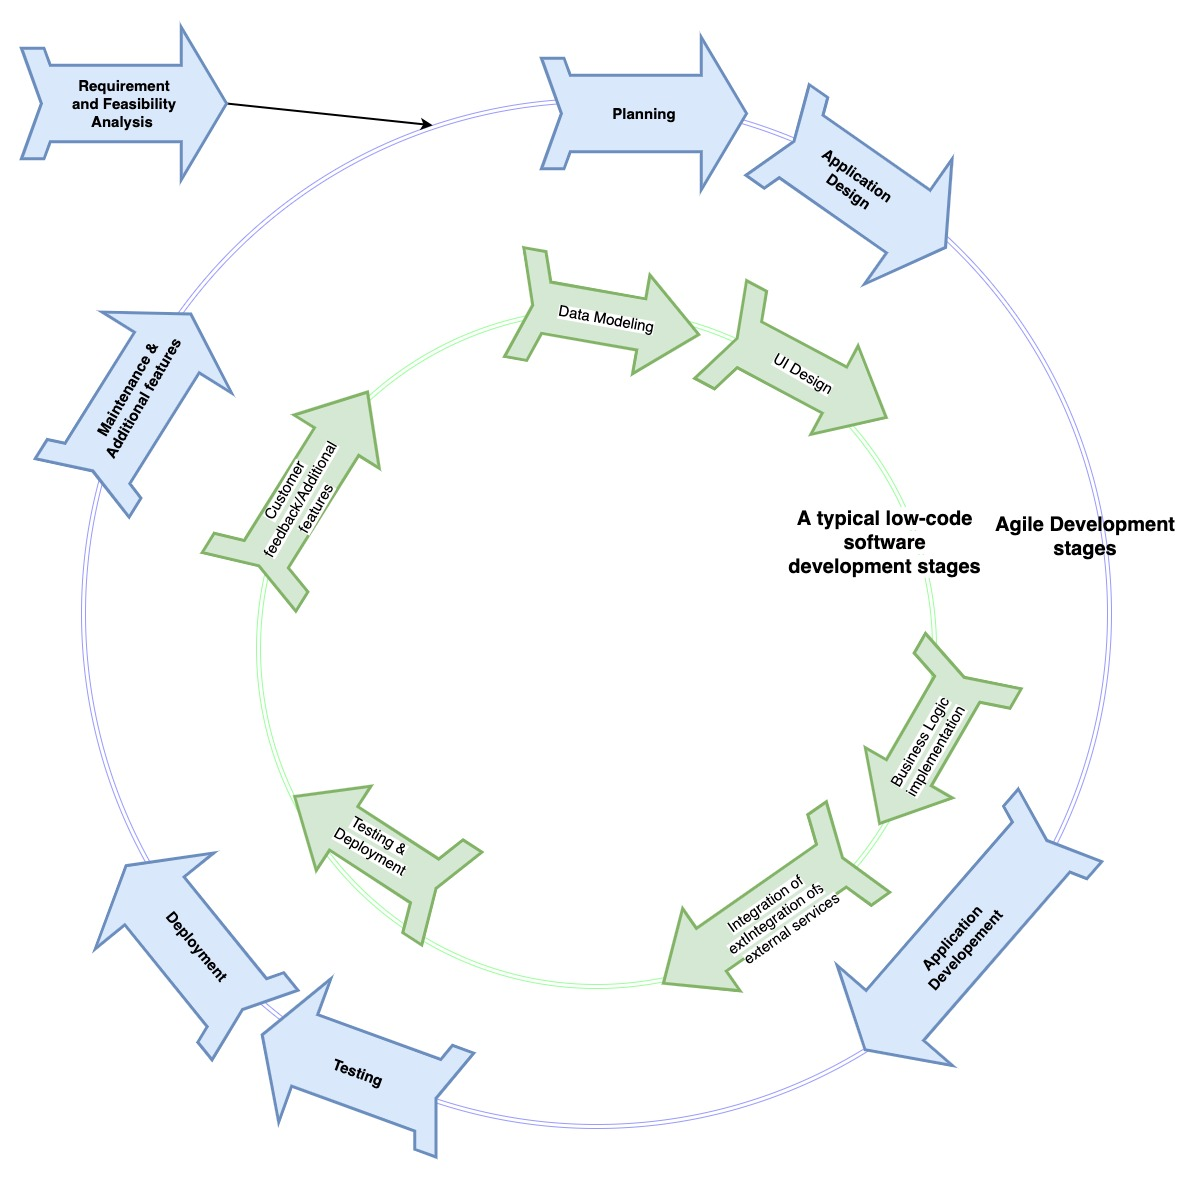
\includegraphics[scale=.22]{res/development_flow-Page-agile_lc.jpg}
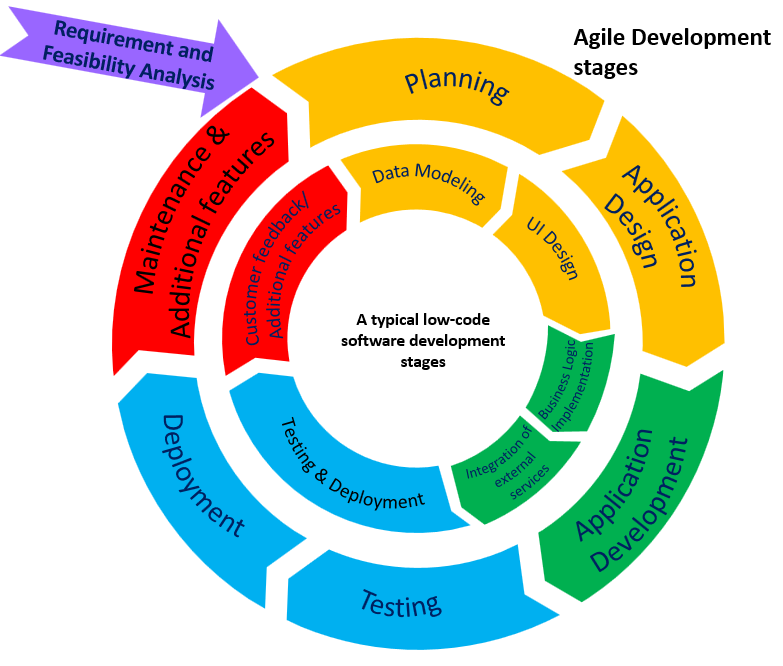
\includegraphics[scale=.50]{res/development_cycle.PNG}
% 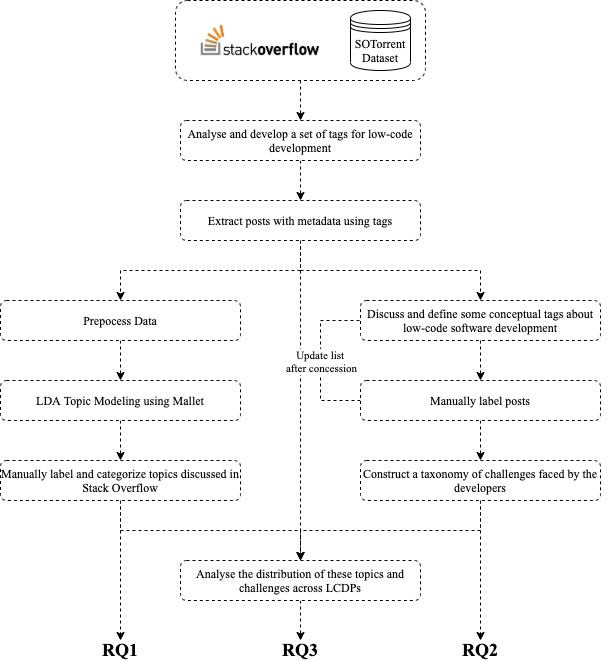
\includegraphics[width=0.35 * linewidth]{res/methology_overview.jpg}
\caption{Agile methodologies in traditional vs  LCSD development}
\label{fig:low-code-agile}
\vspace{-5mm}
\end{figure}

\nd\bf{Development Phases of an  LCSD Application.} A typical  LCSD application can be built in two ways~\cite{sahay2020supporting}: \begin{inparaenum}
\item ``UI to Data Design'', where developers create UI and then connect the UI to necessary data sources, or \item ``Data to UI'' where the design of the data model is followed by the design of the user interfaces. \end{inparaenum} In both approaches, application logic is implemented, and then third party services and APIs are integrated. APIs are interfaces to reusable software libraries~\cite{Robillard-APIProperty-IEEETSE2012}.  
% Application monitoring dashboard, server maintenance, scaling up, etc., are usually supported by the  LCSD platforms. 
A major motivation behind  LCSD is to build applications, get reviews from the users, and incorporate those changes quickly~\cite{waszkowski2019low-automating}. As such, the agile development methodology~\cite{beck2001manifesto} and  LCSD can go hand in hand because the fundamental principle and objective are customer satisfaction and continuous incremental delivery. The inner circle of Figure~\ref{fig:low-code-agile} shows the important development phases of an  LCSD application, as outlined in~\cite{sahay2020supporting}. The outer circle of \fig\ref{fig:low-code-agile} shows the phases in a traditional agile software development environment. As  LCSD platforms take care of many of the application development challenges, some of the agile application development phases have shorter time/execution spans in  LCSD compared to traditional software development. 
%(see \fig\ref{fig:low-code-agile}). 




% \bf{Agile development methodology in low-code application life cycle.}


%\section{Related Work} \label{sec:related_work}


 
%  \subsection{Topic modeling in Software Engineering Research}

% Barua et al.\cite{barua2014developers} conducted a study using LDA topic modeling to gain insightful information regarding developers community and how topics evolve over time in different software domains.
% Rosen et al. \cite{rosen2016mobile} use topic modeling of discussions in Stack Overflow and present popular, difficult topics on mobile development. Yang et al. use topic modeling with ML algorithm to find popular and difficult security topics and categorized them into 5 topics \cite{yang2016security}. Bajaj et al.  \cite{bajaj2014mining} used unsupervised learning to categorize important web development topics, common misconceptions,  and shared and overview of how these questions are evolving over time. Bagherzadeh \& Raffi \cite{bagherzadeh2019going} studied what big data developers asks in SO and their challenges. Adrian et al. used topic modeling on source code to find linguistic topic to find the intention of the code and how these topics are distributed over the system \cite{kuhn2007semantic}. 

% 

%\subsection{Exploratory Study Using SO data}
\section{Study Data Collection and Topic Modeling} \label{sec:methodology}
In this Section, we discuss our data collection process to find  LCSD related posts (Section \ref{data_collection}). We then discuss the details of the topic modeling (Section \ref{topic_modeling}).
 
\subsection{Data Collection} \label{data_collection}
We collect  LCSD related SO posts in three steps: \begin{inparaenum}[(1)]
\item Download SO data dump,
\item Identify  LCSD related tag list, and
\item Extract  LCSD related posts from the data dump based on our selected tag list.
\end{inparaenum} We describe the steps below.

\nd\textbf{Step 1: Download SO data dump.} We downloaded SO data dump~\cite{SOdump} of June 2020. We used the contents of Post.xml file which contained information about each post like the post's unique ID, type (Question or Answer), title, body, associated tags, creation date, view-count, etc. Our data dump included posts from July 2008 to May 2020 and contained around 58,544,636 posts. Out of them, 33.4\% are questions, 66.6\% are answers, and 17.4\% questions had accepted answers.

\nd\textbf{Step 2: Identify low-code tags.}
We need to identify a list of tags that are related to LCSD in order to extract low-code related posts from SO discussions.
In order to find relevant tags, we followed the similar procedure used in prior work \cite{abdellatif2020challenges}, \cite{ahmed2018concurrency}, \cite{wan2019discussed}, and \cite{linares2013exploratory}. At Step 1, we identify the initial low-code related tags and call them $T_{init}$. At Step 2, we finalize our low-code tag list following related work \cite{bagherzadeh2019going}, \cite{yang2016security}. Our final tag list $T_{final}$ contains 19 tags from top nine LCDPs. We discuss each step in details below.

(1) Identifying Initial low-code tags.
The SO posts do not have tags like "low-code" or "lowcode". Instead, we find that  low-code developers use a  LCSD platform name as a tag, e.g., "appmaker" for Google Appmaker~\cite{googleappmaker}. Hence, to find relevant tags, first we compile a list of top  LCSD platforms by analysing list of platforms that are considered as the market leaders in Gartner~\cite{vincent2019magic}, Forrester~\cite{rymer2019forrester}, related research work~\cite{sahay2020supporting}, and other online resources like PC magazine~\cite{pcmag}. We find nine  LCSD platforms are consistently mentioned in the above resources: Zoho Creator~\cite{zohocreator}, Google App Maker~\cite{googleappmaker}, Salesforce Lightning~\cite{salesforce}, Quickbase~\cite{quickbase}, Outsystems~\cite{quickbase}, Mendix~\cite{mendix}, Vinyl~\cite{vinyl}, Appian, and Microsoft Powerapps\cite{powerapps}. %In addition, several other  LCSD platforms are mentioned sporadically in some sources like Kissflow~\cite{kissflow} and ProntoForms~\cite{prontoforms}, but whose discussions are non-existent in our SO data dump. 
We thus focus on the discussions of nine above  LCSD platforms in SO. We find one tag per  LCSD platform as the name of the platform (e.g., "salesforce-lightning"). 
However, upon close inspection of the tags in SO, we found that developers used more than one tag for some of the nine  LCSD platforms. For example, "Microsoft Powerapps" has multiple tags (e.g., "powerapps", "powerapps-formula", "powerapps-canvas"). At the end of our manual inspection, we found total 16 tags for the nine  LCSD platforms. We refer to these 16 tags as $T_{init}$. 

(2) Finalizing low-code related tags.
Intuitively, there might be more variations to tags of nine  LCSD platforms other than those in $T_{init}$. We use heuristics from previous related works~\cite{bagherzadeh2019going},\cite{yang2016security} to find other relevant tags. First, we denote our entire SO dump data as $Q_{all}$. Second, we extract all the questions $Q$ that contain any tag from $T_{init}$. Third, we create a candidate tag list $T_{candidate}$ using all the tags found in questions $Q$. Fourth, we select significantly relevant tags from  $T_{candidate}$ for our  LCSD discussions. To find relevant tags, we use heuristics from previous related work \cite{bagherzadeh2019going}, \cite{yang2016security}. We compute significance and relevance for each tag $t$ in $T_{candidate}$ with respect to $Q$ (our extracted questions that has $T_{init}$ tag) and $Q_{all}$ (i.e., our data dump) as follows,
{ \[
( Significance) \ \ S_{tag} \ =\ \ \frac{\#\ of\ ques.\ with\ the\ tag\ t\ in\ Q}{\ \ \#\ of\ ques.\ with\ the\ tag\ t\ in\ Q_{all}}
\]

\[
% ( Relevance) \ \ \mv \ =\ \ \frac{\#\ of\ questions \ with\ the\ tag\ t\ in\ Q}{\ \ \#\ of\ the\ questions\ in\ P}
( Relevance) \ \ R_{tag} \ =\ \ \frac{\#\ of\ questions\ with\ tag\ t\ in\ Q}{\ \ \#\ of\ questions\ in\ Q}
\]} A tag t is significantly relevant to  LCSD development if the $S_{tag}$ and  $R_{tag}$ are higher than a threshold value. We experimented with a wide range of values of $S_{tag}$ and  $R_{tag}$. We found relevant tag set for  LCSD development for $S_{tag}$ = 0.2 and $R_{tag}$ = 0.005 . These values are consistent with related work~\cite{Bagherzadeh-BigdataTopic-FSE2019,ahmed2018concurrency}. The final tag list $T_{final}$ contains 19 significantly relevant tags. 
%that also contains the 16 tags from $T_{init}$.


\nd\textbf{Step 3: Extracting low-code related posts.}
An SO question can have at most five tags, and we consider a question as low-code related question if at least one of it's tag is in our chosen tag list $T_{final}$. Based on our $T_{final}$ tag set, we found a total 7,302 posts from our data dump. There were 51.3\% Questions (i.e., 3,747) and 48.7\% Answers (i.e., 3,555) and among them 16.9\% Questions (i.e., 1,236) had accepted answers. SO has a score-based system (upvote and downvote) to ensure the questions are in proper language with necessary information (code samples and error messages), not repeated or off-topic. Here is an example for a question with score "-4" where a practitioner is making an API related query in Powerapps(\dq{61147923})\footnote{$Q_i$ and $A_i$ denote a question Q or answer A in SO with an ID $i$} platform. However, it is not clear what the practitioner is asking as the question is poorly written and without any clear example. In order to ensure good quality discussions, we excluded questions that had a negative score which resulted in 6,982 posts containing 51.5\% Questions (i.e., 3,597 ) and 48.5\% Answers (i.e., 3,385). Following previous research \cite{bagherzadeh2019going}, \cite{rosen2016mobile}, \cite{barua2014developers}, we excluded unaccepted answers and only considered accepted answers for our dataset. Hence, our final dataset $B$ contained  4,785 posts in total containing 3,597 non-negative scored questions and 1,188 accepted answers. 
%and their metadata to conduct this study. 



\subsection{Topic Modeling} \label{topic_modeling}
We produce  LCSD topics from our extracted posts in three steps: \begin{inparaenum}[(1)]
\item Preprocess the posts, 
\item Find optimal number of topics, and
\item Generate topics.
\end{inparaenum} We discuss the steps below.

\nd\textbf{Step 1. Preprocess the posts.} For each post text, we remove noise following related works \cite{abdellatif2020challenges,bagherzadeh2019going,barua2014developers}. First, we remove the code snippets from the body which is inside \textless code\textgreater \textless /code\textgreater\ tag, HTML tags such as (\textless p\textgreater \textless /p\textgreater, \textless a\textgreater \textless /a\textgreater, \textless li\textgreater \textless /li\textgreater\ etc), URLs. Then we remove the stop words such as "the", "is", "are", punctuation marks, numbers, non-alphabetical characters using the stop word list from MALLET\cite{mccallum2002mallet}, NLTK\cite{loper2002nltk}, and our custom low-code specific (i.e.,  LCSD platform names) stop word list. After this, we use porter stemmer\cite{ramasubramanian2013effective} to get the stemmed representations of the words e.g., "wait", "waits", "waiting", "waited" - all of which are stemmed to base form "wait".

\nd\textbf{Step 2. Finding the optimal number of topics.}  After the prepossessing, we use Latent Dirichlet Allocation  \cite{blei2003latent} and the MALLET tool \cite{mccallum2002mallet} to find out the  LCSD related topics in SO discussions. We follow similar studies in Software engineering research using topic modeling \cite{arun2010finding, asuncion2010software, yang2016security, bagherzadeh2019going,abdellatif2020challenges}. Our goal is to find the optimal number of topics $K$ for our dataset $B$ so that the \textit{coherence} score i.e., encapsulation of underlying topics is high. we use Gensim package \cite{rehurek2010software} to determine the coherence score following previous works \cite{uddin2017automatic, roder2015exploring}. We experiment different values of $K$ that ranges from \{5, 6, 7, .. ,29, 30\} and for each value we run  MALLET LDA on our dataset for 1000 iterations \cite{bagherzadeh2019going}. Then we observe how the coherence score is changing with respect to $K$. We pick the topic model with the highest coherence score. Choosing the right value of $K$ is important because, for smaller values of $K$, multiple real-world concepts merge, and for a large value of $K$ a topic breaks down. For example, in our result, the highest coherence score 0.50  for $K$ = 7 and $K$ = 13. We choose $K$ = 13 as it captures our underlying topics better. For $K$ = 7, we find that it merge topic 'Dynamic Event Handling', 'Dynamic Content Display', and 'Dynamic Form Controller'. MALLET also uses two hyper-parameters $\alpha$ and $\beta$ to distribute words and posts across the topics. Following the previous works~\cite{bagherzadeh2019going, ahmed2018concurrency, bajaj2014mining, rosen2016mobile}, we use the standard values $50/K$ and 0.01 for hyper-parameters $\alpha$ and $\beta$ in our experiment.  

\nd\textbf{Step 3. Generating topics.} Topic modeling is a method of extracting a set of topics by analysing a collection of documents without any predefined taxonomy. Each document has a probability distribution of topics, and every topic has a probability distribution of a set of related words \cite{barua2014developers}. We produced 13 topics using the above LDA configuration on our dataset $B$. Each topic model offers a list of top $N$ words and a list of $M$ posts associated with the topic. In our settings, a topic consists of 30 most frequently co-related words which represents a concept. Each post had a correlation score between 0 to 1, and following the previous work \cite{wan2019discussed}, we assign a document with a topic that it correlates most.  







% https://stackoverflow.com/questions/61147923/how-to-parameterize-api-url-in-powerapps
% \paragraph{Step 4: LDA Topic Modeling.}
% 
% \textit{Preprocess the posts} 
% Before we run the topic modeling on our extracted questions, we need to preprocess them. For the topic modeling we used posts title, body and accepted answers. Then we followed the following steps to remove noise from our documents following related works \cite{abdellatif2020challenges} \cite{bagherzadeh2019going} \cite{barua2014developers}. First we remove the code snippets from the body which is inside \textless code\textgreater \textless /code\textgreater\ tag, HTML tags (\textless p\textgreater \textless /p\textgreater, \textless a\textgreater \textless /a\textgreater, \textless li\textgreater \textless /li\textgreater\ etc), URLs. Then we remove the stop words such as "the", "is", "are", punctuation marks, numbers, non-alphabetical characters using the MALLET'S stop word list\cite{} and ?. After this we use stemmer to get the stemmed representations of the words e.g., "wait", "waits", "waiting", "waited" all were stemmed to base form "wait".
% % prunning remove words appeared more than ? percent or less than ? percent
% % to preprocess i.e. stop words removal, lematization, prunning etc. We followed the best guidelines on how to apply topic modeling in Software Engineering research\cite{chen2016survey}
% 
% 
% \textit{Topic modeling settings}
% % Defination of topic modeling
% Topic modeling is a method of extracting a set of topics by analysing a collection of documents \cite{wiki1} without any predefined taxonomy. In this method each document has a probability distribution of topics and every topic has a probability distribution of set of related words \cite{barua2014developers}. For example, we have a topic called ? which consists of high frequency words such as ?,? ,? ? etc. 
% 
% % Topic modeling tools, configuration, settings, and some results
% After the prepossessing, we used Latent Dirichlet Allocation  \cite{blei2003latent} and the MALLET tool \cite{mccallum2002mallet} to find out the low-code development related topics that are discussed on SO. We followed similar studies in Software engineering research using topic modeling \cite{asuncion2010software} \cite{yang2016security} \cite{bagherzadeh2019going} \cite{abdellatif2020challenges}. 
% 
%  Choosing the right value of K is important because for smaller value of K multiple different real world concepts will be merged and for large value of K a topic will be broken down to some subtopic. For example when we used K = ? ? and ? topic were merged into one. And when we used K = ?, ? topic was divided into ? and ? subtopic. In our experiments we experiments, we tried different values of K ranges from {5, 6, .? ? ?. , 30}. and I = {1, 43,243 ,? ? }. We used coherence metric value to find for which value of K the topics have more understand-ability \cite{roder2015exploring}. We found that when K value ranges ? to ? the coherence score is very high and almost same. Based of manual observation of top ? topics we found that for K=? the model generates good topics for our low-code dataset. For MALLET configuration we used the standard values 50/K and 0.01 for hyper-parameters $\alpha$ and $\beta$  which provided good results for us following previous work \cite{bagherzadeh2019going} \cite{ahmed2018concurrency} \cite{bajaj2014mining} \cite{rosen2016mobile}. In our settings, a topic consists of ? most frequently co-related used words which represents a concept. After ? iteration the Mallet returns a K topics and each topic consists of ? words.
% 
% 
% \textit{Labeling topics}
% LDA usually captures topic by analysing SO discussions without proper understanding of domain-specific concepts. 
% Mallet does not provide a meaningful title for the topic, it only returns a set of co-related words. 
% % We need to name to K topics returned by the Mallet a meaningful name.
% We need to categorize the K LDA topics on technical discussions returned by the MALLET to match higher level concepts. For example, a topic with group of words were ...??... 
% 
% From previous works \cite{}\cite{} \cite{} we used open card sort \cite{fincher2005making} to label the $K$ topics. In this way we inspected ? words in each topic and read top ? posts associated with that topic to come up with a topic name. From the $K$ topics we merged topic ? with topic ? because after analysing the posts it seemed like they were basically mentioning same things. The topics were discussed by all the authors in. In order to categorize topics into higher level category we grouped similar topics. For example topic ? and topic ? were grouped into ? higher level topic. Table \ref{} shows the summary of topic names, high level category name, favorite count, number of posts in each topic etc.
% 
% 
% % LDA also provided to find similarity of between topics
% 
% 
% 
% 
% \paragraph{Step 5: Manually label questions to understand practitioner's challenges}
% Manually labelling the questions to understand the challenges the low-code application practitioners are facing was the most time consuming part of this study. We conducted X round of meetings over X months to plan, discuss and resolve conflicts. At the end we need less regular meetings because we were already in sync. In total we reviewed X number of SO questions and among them around X\% of questions required conflict resolution meeting. 
% 
% We analysed and labeled the extracted posts by four authors in a open coding procedure \cite{seaman1999qualitative}. The questions extracted at step 3, were divided among three authors who labeled a question by providing a description of the challenge. The number of labels were growing very diverse as there are not much clarification and guidelines to categorize the low-code development challenges. So we decided to label each question on a fixed list of tags. Initially we started with 84 tags summarized from authors' label of the challenge. Some of this tags very closely related for example ? ? ?.  We routinely held meetings and updated this list either by introducing new tags or merging some of the existing tags together. For example we merged ? and ? to ? because they were closely related. Again after labeling a few questions we introduced ? tag because we saw there were lots of questions regarding that. This way we were able to maintain a consistent naming without suffering a significant bias \cite{humbatova2020taxonomy}.
% 
% The goal of this manual review of SO discussion was to fully understand what sort of challenges the practitioners are facing, so we studied the questions along with answers and comments to fully understand the real issue and provide a label to it. We spent around 3 hours for the questions labeling and resolving conflicts. There were some questions which were vague to understand which we labeled ?. We rigorously followed procedures in labelling the questions, specially for the tricky situations like 1. Questions was not related low-code application rather some general programming language related. 2. authors did not understand how to tag/label this question.
% 
% A final meeting was held and we reviewed the tag list and number of questions in each tag. We merged some of tags that had relatively very low number of questions.
% 
% % Some of the questions are tagged wrongly because the citizen developers do not have enough domain knowledge to tag appropriately. Applying right tag is important to get proper support from community experts \cite{bangash2019developers}.
% 
% % open card sorting \cite{spencer2009card}
% 
% 
% 
% \paragraph{Step 6: Taxonomy of challenges Construction \& Validation.}
% 
% % \begin{figure*}[htb]
% % \centering
% % 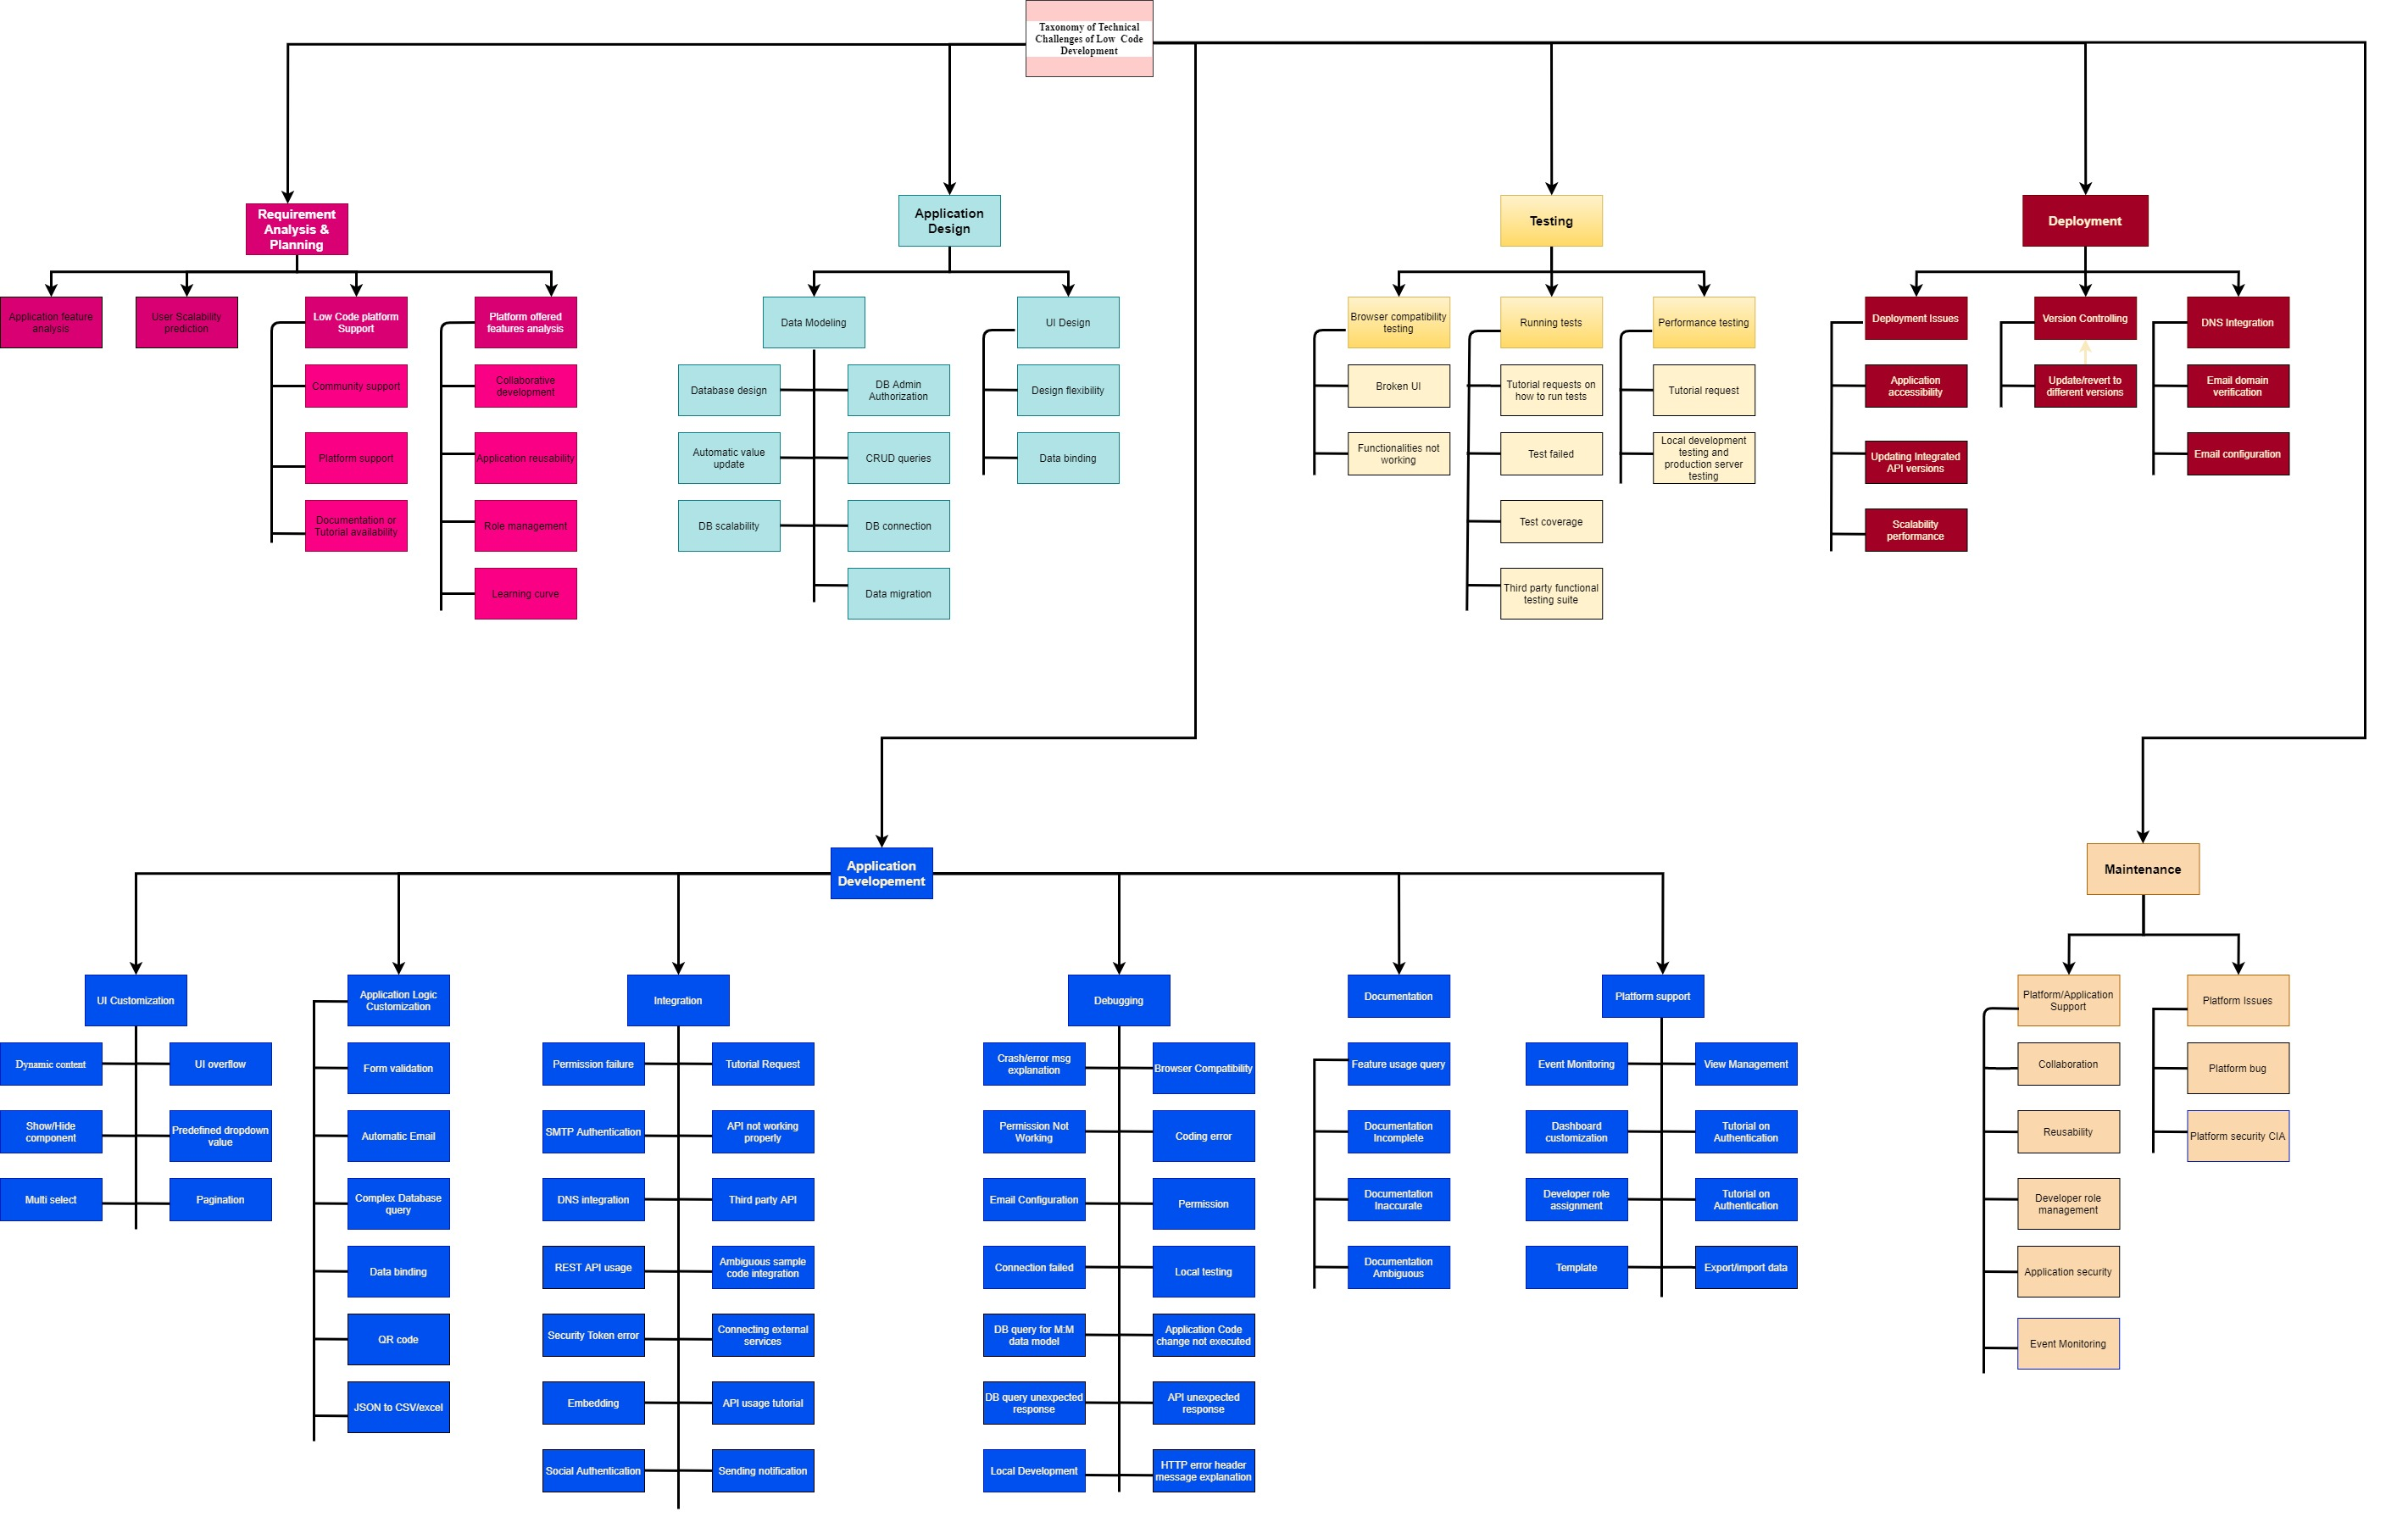
\includegraphics[scale=0.17]{res/LowCodeChallenges.jpg}
% % % 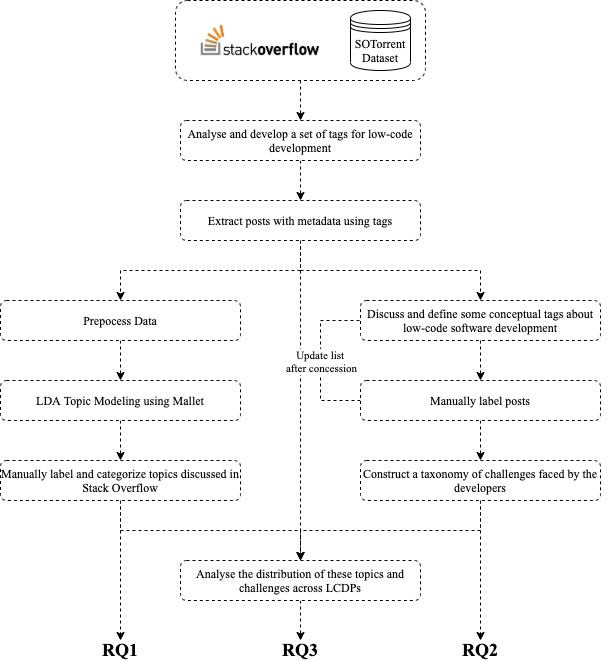
\includegraphics[width=0.35 * linewidth]{res/methology_overview.jpg}
% % \caption{Taxonomy of challenges that low-code practitioners face during different life cycle of application development}
% % \label{fig:taxonomoy_low_code_challenges}
% % \end{figure*}
% 
% we built the taxonomy is a bottom up approach\cite{humbatova2020taxonomy}. First we created a group for similar tags and then we created a high-level classification of the parent category. Each classification was validated by all the authors in a group meeting. At the end all of the authors reviews the categories, subcategories and sub sub categories and made some final changes.
% 
% We organized our taxonomy based the challenges practitioners face during different phases of application development . Our taxonomy consists of ? higher level category resembling the ? stages of agile software development life cycle. Each SDLC stage contains some sub-category of challenges that low-code practitioners have discussed on SO. There are total ? sub category of challenges such as ? ? ?. Each of this sub-category contains some low level low-code technology related challenges i.e. tags. In total there are ? low level tags. Figure \ref{sec:taxonomy}.
% 
% The final taxonomy is reviewed and agreed with all the authors. We had some reservations with the initial taxonomy that we resolved by discussing it with each other.
% 
% 
% \paragraph{Step 7: Analyze discussions and challenges across LCDPs.}
% 
% 
% 
% % From our extracted data we found that in total ? LCDPs are discussed in SO. 
% 




\section{Empirical Study} \label{sec:results}
We answer three research questions by analyzing Low Code Software Development (LCSD)  discussions in SO.
\begin{enumerate}[leftmargin=30pt, label=\bf{RQ\arabic{*}.}]
  \item What types of topics are discussed about LCSD? 
  \item How are the topics distributed across low-code SDLC? 
  \item What LCSD topics are the most difficult to answer?
  %\item How do the topics vary across the different low code software providers?
  %\item What types of questions are asked about low code software in Stack Overflow?
  %\item How do the popularity and difficulty of the topics vary in Stack Overflow?
  %\item How do the topics evolve over time in Stack Overflow?
\end{enumerate}
The first research question aims to understand the types of topics discussed in
SO about LCSD (\sec\ref{sec:rq-topic-type}). The second research
question aims to understand how each topic is discussed across different stages of low-code SDLC (software development life cycle) (\sec\ref{sec:rq-topic-challenges}). The third research question offers insight into the challenges of LCSD 
developers across the observed LCSD topics based on the measurement of difficulty of getting answers (\sec\ref{sec:rq-topic-difficulty}).


\subsection{What types of topics are discussed about LCSD? (RQ1)}\label{sec:rq-topic-type}

 

% \begin{figure}[htb]
% \centering
% 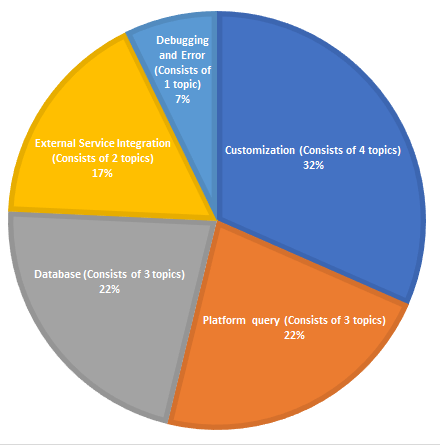
\includegraphics[scale=0.90]{res/PieChart.png}
% % 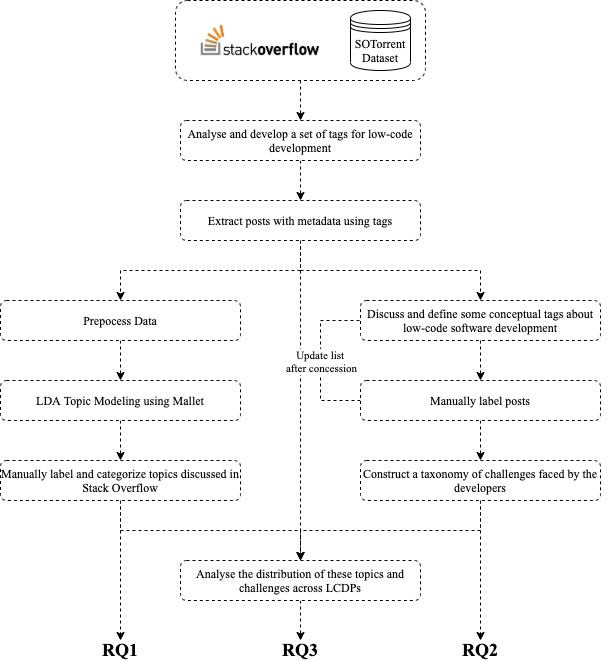
\includegraphics[width=0.35 * linewidth]{res/methology_overview.jpg}
% \caption{ Distribution of percentage of questions and topics per higher level category}
% \label{fig:distribution_of_questions_topic_pie_chart}
% \end{figure}
% \subsubsection{Motivation}
% Low-code software development is becoming more and more popular as a flexible
% and easy approach to develop useful business applications. In many ways low-code
% software development is different from traditional software development. Being a
% recent trend, the challenges of low-code development are yet to be studied well
% as observed in discussed in \sec\ref{sec:related_work}. SO is an established source of knowledge repository that can
% be used for the systematic study of the real world challenges faced by the
% practitioners. Hence, the low-code related SO data mined as described in Section
% \ref{sec:methodology} offers us the opportunity to analyze topics of discussions
% of the low-code practitioners. Investigating this first research question will
% help LCSD platform developers and researchers to have better understanding of
% prevalent issues and improve the quality of LCSD technology.

\subsubsection{Approach}
We get 13 low-code related topics from our LDA topic modeling as discussed in \sec\ref{sec:methodology}. We use card sorting \cite{fincher2005making} to label these topics  following previous
works \cite{bagherzadeh2019going, ahmed2018concurrency, yang2016security, rosen2016mobile, abdellatif2020challenges}.
In open card sorting, there is no predefined list of labels. To label a topics, 
we used the top 30 words for the topic and a random sample of at least 20 questions that are assigned to the topic. Four of the authors participated in the labelling process.
Each author assigns a label for each topic and discusses with each other until
there is an agreement. The authors reached an agreement after around 15
iterations of meetings over Skype and email and labeled the 13 topics from the
LDA output discussed in Section \ref{sec:background}. After the labeling of the topics, we grouped them into higher categories. For
example, UI Adaptation and Dynamic Form Controller are related to UI design, and
so we group them into a group named UI. In the same way, Dynamic Event Handling,
Dynamic Content Display, and Dynamic Content Binding topics are related to the
middleware feature of low-code development platforms, and so we put these three
topics into Middleware sub-category. We repeat these process until we can not
find any more higher-level group. For example, the above mentioned two
categories UI and Middleware belong to the application customization task where
the developers customize the UI or the business logic of the application
according to their need. Hence, we put them under a high-level category named
Customization. Similarly, we put Access Control \& Security into Configuration sub-category. Then we put Configuration sub-category and Client Server Comm \& IO topic under Platform Adaptation high-level category.

% Similarly, we put SQL CRUD into Management sub-category and Data
% Storage \& Migration to Migration sub-category and then put these two
% sub-categories under a higher category named Database.


\begin{figure}[t]
	\centering\begin{tikzpicture}[scale=0.28]-
    \pie[
        /tikz/every pin/.style={align=center},
        text=pin, number in legend,
        explode=0.0,
        color={black!0, black!10, black!20, black!30,, black!40},
        ]
        {
            17/\bf{Third-Party}\\Integration\\ (17\%Q 2T),
            40/\bf{Customization}\\UI or Service (40\%Q 5T),
            22/\bf{Platform}\\ Adoption (22\%Q 3T),
            22/\bf{Database}\\Management\\ (22\%Q 3T)
        }
    \end{tikzpicture}
	\caption{Distribution of questions (Q) and topics (T) per topic category}
	\vspace{-5mm}
	\label{fig:distribution_of_questions_topic_pie_chart}
\end{figure}

\begin{figure}[t]
\centering
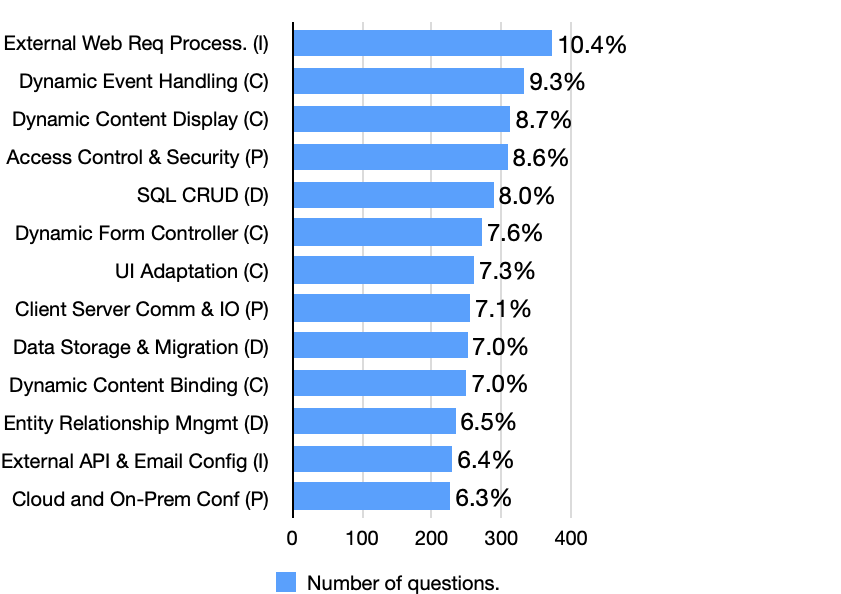
\includegraphics[scale=0.32]{res/barChart.png}
% 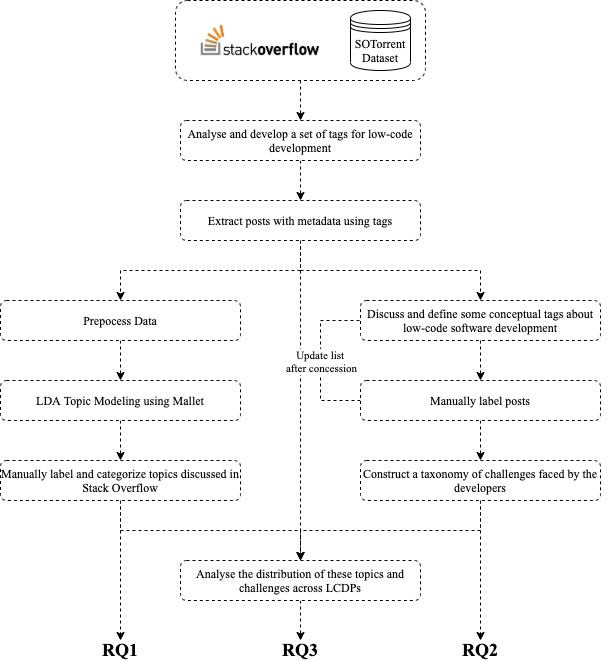
\includegraphics[width=0.35 * linewidth]{res/methology_overview.jpg}
\caption{Distribution of questions by low-code Topics (C = Customization Category, I = Integration, P = Platform Adoption, D = Database)}
\label{fig:distribution_of_questions_topic_bar_chart}
\end{figure}
\subsubsection{Results}

\begin{figure}[t]
\centering
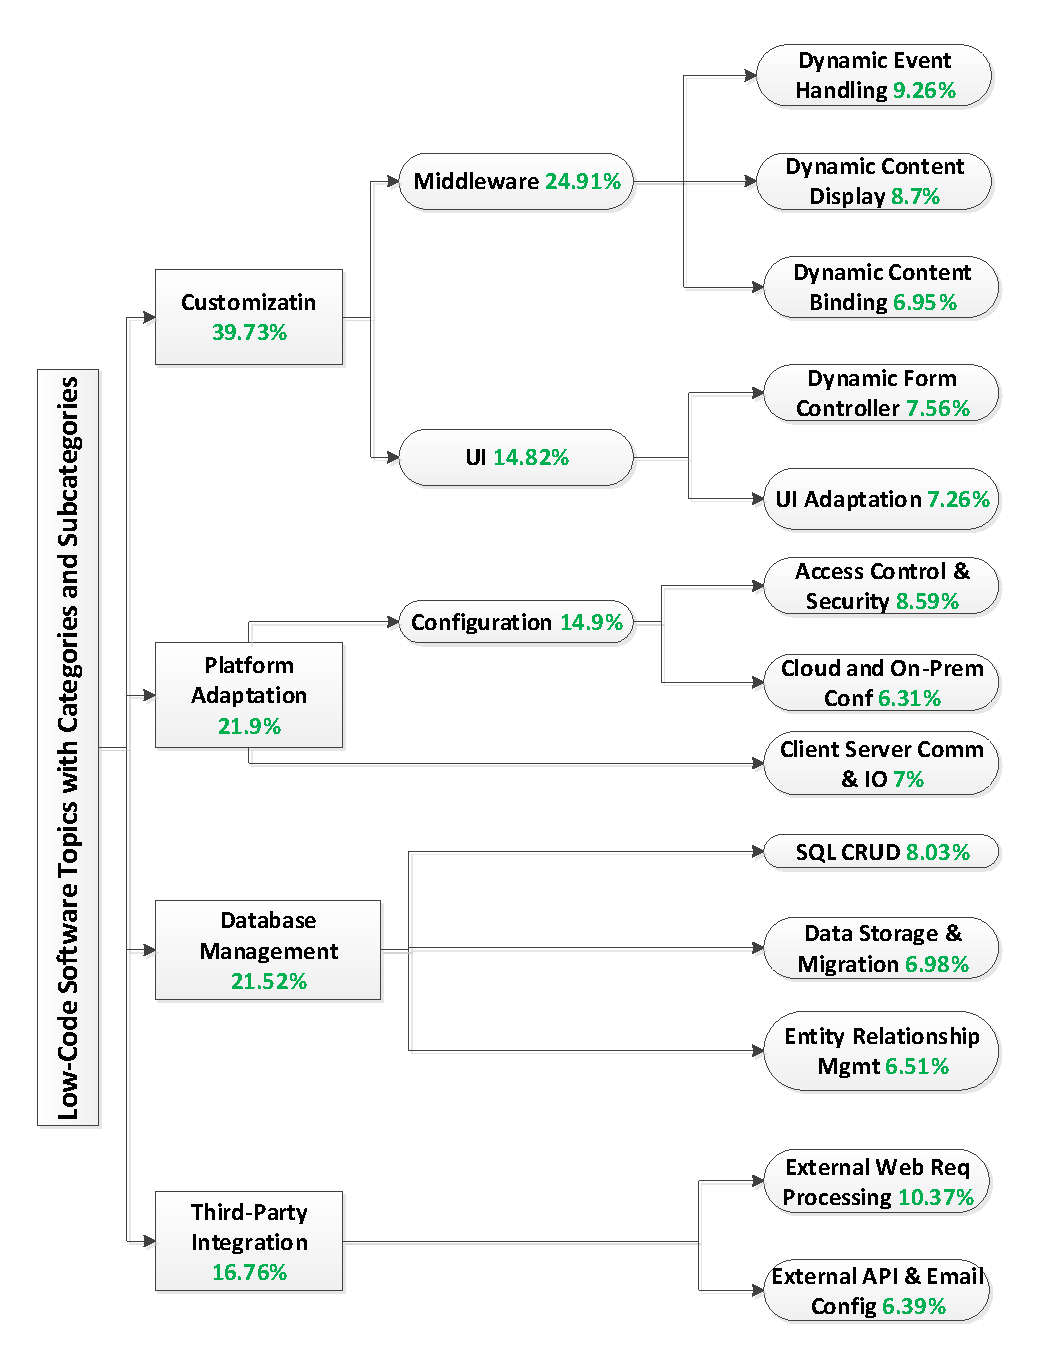
\includegraphics[scale=0.48]{res/TM_taxonomy.pdf}
% 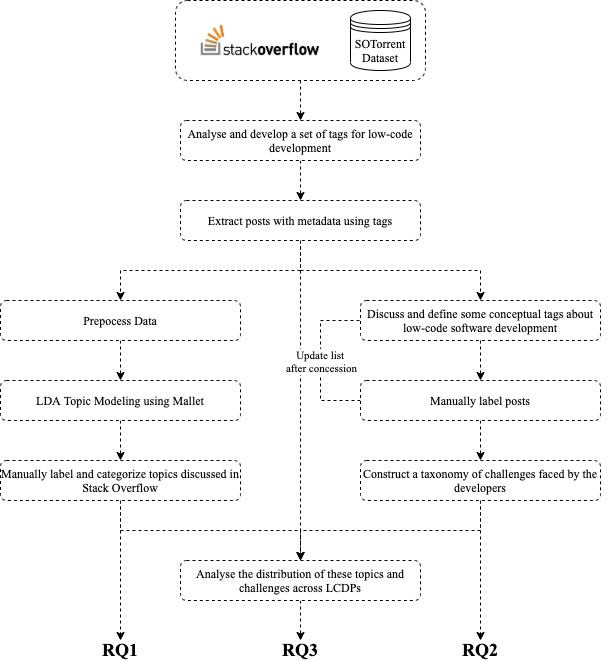
\includegraphics[width=0.35 * linewidth]{res/methology_overview.jpg}
\caption{ Low-code topics categories and sub-categories}
\label{fig:taxonomy_TM}
\end{figure}




We find 13 LCSD topics that we group into four high-level categories: \textbf{Customization, Platform Adoption, Database Management, and Third-Party Integration.} \fig\ref{fig:distribution_of_questions_topic_pie_chart} shows the distribution of
questions and topics among the four high-level categories. The \textit{Customization} category 
covers the highest percentage of questions
and number of topics (40\% questions and five topics), followed by \textit{ Platform Adoption} (22\%
questions and three topics), \textit{Database Management} (33\% questions and three topics), and \textit{Integration}
(17\% questions and two topics). \fig\ref{fig:distribution_of_questions_topic_bar_chart} sorts the 13 topics based on number of questions. The
\textit{'External Web Req Processing topic'} covers the most questions regarding queries and discussions related
to the integration of third party services/APIs (10.4\%). The \textit{'Dynamic Event Handling'} has the second most questions (9.3\%) related to the implementation of business logic.

In Figure \ref{fig:taxonomy_TM}, we group the 13 topics into four high-level categories. The categories are sorted according to the number of
questions belonging to them. For example, the topmost category \textit{Customization} has the most number of questions under them. Each category may consist of some
sub-categories. For example, \textit{Customization} Category contains two sub-categories:
\begin{inparaenum}[(1)]
\item \textit{Middleware},
\item \textit{UI}
\end{inparaenum}. Each sub-category contains one or more topics. For example,
Middleware sub-category consists of three topics: \begin{inparaenum}[(1)] \item
Dynamic Event Handling, \item Dynamic Content Display, \item and Dynamic content
Binding \end{inparaenum}. Each sub-category and topic are organized according to
their distribution of questions. For example, under Customization (40\%)
category, \textit{Middleware} (25\%) is followed by \textit{UI} (15\%) sub-category. In the same
way, 'Dynamic Event Handling' (9.3\%) topic is followed by 'Dynamic Content
Display' (8.7\%) topic based on their question distribution.



% \begin{inparaenum}[(1)]
% \item 
% \item 
% \end{inparaenum}


% \nd\bf{$\bullet$ Software Related Topics.} Out of the 40 topics, 19 topics belong to the Software category. These topics contain discussions about the 
% the usage, processing and troubleshooting of IoT software, libraries, and data. 
% The topics are grouped into three sub-categories: \begin{inparaenum}[(1)]
% \item Platform management topics contain discussions related to the IoT platforms (serivces, operating systems, SDKs, etc.),
% \item Troubleshooting topics are about the debugging of source code and the underlying IoT platforms, 
% \item Data parsing topics contain discussions about the processing of multimedia and textual contents in IoT devices.  
% \end{inparaenum} %We discuss the topics by the three sub-categories below.

\nd\bf{$\bullet$ Customization} is the largest category with 40\% of the SO posts and five topics. It contains discussions about business
logic implementation, input and form validation, linking the UI to the backend
storage via dynamic content binding, a drop-down menu with predefined value,
formatting date and time, drop-down widgets, etc. It contains two sub-categories
of topics: \begin{inparaenum}[(1)] \item \textit{UI} sub-category contains discussions
on drag-and-drop UI and form design and also customization of UI components,
\item \textit{Middleware} sub-category covers discussions on the middlewares that
provide support for system integration, the connection between UI and storage layer, etc.
%\anindya{How scalability and authentication are related to middleware is not clear. A bit of explanation would help.}
% \item Data parsing topics contain discussions about the processing of multimedia and textual contents in IoT devices.  
\end{inparaenum}

\bf{{Middleware (25\% questions)}} sub-category contains three topics:
\begin{inparaenum}[(1)] \item \it{Dynamic Event Handling (9.26\%)} has
discussions about handling user interaction events, accessing input
value after form submission (\dq{43096166}) rendering chart in the
canvas(\dq{56154215}).
%, parent component handling child component
%events(\dq{57982913}).
\item \it{Dynamic Content Display (8.70\%)} is about dynamically displaying
items on the page (\dq{53648077}), displaying content based on previous action,
creating and accessing gallery from multiple data sources (\dq{51764889}).
\item \it{Dynamic Content Binding (6.95\%)} is about updating views when some
other values get changed (\dq{59932262}) and building process based on some values
on the form (\dq{61282976}).
\end{inparaenum} 

\bf{{UI (15\% questions)}} sub-category contains two topics:
\begin{inparaenum}[(1)] \item \it{Dynamic Form Controller (7.56\%)} contains
discussions related to the design of forms with predefined values and the implementation of multi-select and customized drop-down values (\dq{44013975}), adding event-listeners to text
widget (\dq{46038130}), etc.
\item \it{UI Adaptation (7.26\%)} is about designing and customizing the user
interface using the graphical interface,
resizing console panel (\dq{34515865}).
\end{inparaenum} 

% For example, in \dq{41438021} a practitioner is about a cross origin issue and he was getting this issue because during the Ajax request the practitioners did not add the "crossOrigin: true" in the HTTP post header.

% Customization is the biggest category of topics and it contains around ?\% of documents of our topic modeling dataset. It contains four topics namely UI customization, Application customization \& Testing, Input \& form validation, Dynamic content and Data binding. The Customization category consists discussions mainly UI design and custom business logic implementation, input validation, design forms, linking the UI to the backend storage via dynamic content binding, drop-down menu with predefined value, formatting date time, drop down widgets running some basic tests. Application customization and testing topic has the highest number of average view count. Discussions in this category suggest that many practitioners lack proper programming background and task based tutorial is highly useful. For example, a practitioner is asking how to add event listener to a widget e.g., "Event Listener for App Maker Text Editor Widget" (\dq{46038130})



\nd\bf{$\bullet$ Platform  Adoption} is the second-largest category with 22\% of questions. It contains discussions about generic query on LCSD platform features
and support, role management, SDLC management tools (e.g., scrum, agile), cloud setup and configuration, deployment issues, etc. The category has three topics. One topic \it{Client Server Comm \& IO (7.09\%)} contains discussions on client-server architecture (\dq{54900592}), debugging server-side
scripts(\dq{55283256}), and general debugging queries on error messages or
unexpected output (\dq{50936643}). The other two topics are grouped under Configuration sub-category. 

\bf{{Configuration (15\% questions)}} contains discussions on LCSD platform configuration on access control and cloud-based setup. There are two topics:
\begin{inparaenum}[(1)] \item \it{Access Control \& Security (8.59\%)} is about
discussion on role-based access control to tasks (\dq{51431318}), Configuration of existing
authentication mechanism (Azure Active Directory configuration (\dq{61734680}).
\item \it{Cloud and On-Prem Conf (6.31\%)} contains discussion on the proper configuration parameters and 
guidelines to connect to the cloud/on-prem databases (\dq{55207558} \dq{45740520}).
\end{inparaenum} 



% \textbf{Platform  Adoption.}
% This high level category consists of three topics namely Platform services and Cloud configuration, Tutorial or Documentation, Deployment and Role management from our LDA modeling. Practitioners ask question on generic query on LCDPs,  what sort of features they LCDPs provide and their limitations, tutorial request on how to do a particular tasks,  cloud server configuration,  platform support on deployment and developers role management, cloud settings, different security and permission for deployment. This category consist of ?\% of total post of our dataset. Different platform provides support on version controlling, provides role management for collaborating development. Some LCDPs provides visual tools to track the progress of the application development. Some platforms also support SDLC management tools such as agile, scrum, kanban \cite{sahay2020supporting} to easy planning, tracking, and collaboration.

% % \bf{{Middleware (25\% questions)}} sub-category contains three topics: 
% \begin{inparaenum}[(1)]
% \item \ib{Dynamic Event Handling (9.26\%)} contains discussions (\dq{}), (\dq{}).
% \item \ib{Dynamic Content Display (8.7\%)} is about  (\dq{}),  (\dq{}).
% \item \ib{Dynamic Content Binding (6.95\%)} is about  (\dq{}),  (\dq{}).
% \end{inparaenum} 

\nd\bf{$\bullet$ Database} is tied to the second biggest category with 22\% of questions. It contains discussions about database connection, SQL CRUD
operations, import/export existing data, etc. There are three topics:
\begin{inparaenum}[(1)] \item \it{SQL CRUD (8.03\%)} contains discussions on SQL
query (\dq{49051500}, \dq{59852901}) and table joining(\dq{37707699}).
\item \it{Data Storage \& Migration (6.98\%)} discusses the upload
and storing of files on the server (\dq{49666940}), moving files from one platform
to another(\dq{55726281}), conversion of large CSV files to excel sheet
(\dq{50977178}), etc.
\item \it{Entity Relationship Management (6.51\%)} contains discussion on
relational database design  (\dq{51881224}) and platform support/limitations
on relational database (\dq{58935331}).
\end{inparaenum} 

% For example in \dq{34341952} a developer asking about an error while inserting new row (e.g., "Cannot insert duplicate key row in object with unique index . The duplicate key value. The statement has been terminated").


% \textbf{Database.}
% This category contains technical discussions related to backend storage design, platform support and limitation of database performance and scalability. Database is the second biggest category of topics and it contains around ?\% of documents of our topic modeling dataset. It consists of three topics namely Storage \& Data migration, Database query, and Platform support on database design. LCDPs usually connect with both SQL or NoSQL based databases. Database scalability, query optimizations, availability related complexity is abstracted from the users and in this category the discussions are more focused on how to do some CRUD operations, import/export existing data. Here a practitioner who is new to Database and low-code platform asking questions regarding how to create a duplicate value. He was getting an error because the field has unique attribute. This is a general concept in database but many of the low-code practitioners do not have strong programmatic background. "Cannot insert duplicate key row in object with unique index . The duplicate key value. The statement has been terminated" (\dq{34341952}). In this questions also asking very common database query. "SOQL - Querying for a list of users the current user is following" (\dq{9168994}).


\nd\bf{$\bullet$ Integration} around 17\% of documents and two topics. It contains discussions about email server configuration, integration
of external services, OAuth, fetching and parsing data, etc. It contains two
topics: \begin{inparaenum}[(1)] \item \it{External Web Req Processing (10.37\%)}
contains posts regarding API integration, parsing and bugging the response of
REST API (\dq{21314917}), and OAuth (\dq{56873258}), some general query on
networking protocols such as HTTP, REST API (\dq{48628269}), etc.
\item \it{External API \& Email Config (6.39\%)} is about configuration, sending
or forwarding emails (\dq{34085695}), configuration error (\dq{31501424}), how
to use generic programming language to send email (\dq{36341976}), creating
managing calendar events (\dq{46738962}), etc.
\end{inparaenum} 

% \textbf{Integration.}
% LCDPs provide developers APIs to interact with the platform and integrate different functionalities. All the challenges regarding load balancing, deploying and managing micro-services are hidden. Developers can integrate external APIs by some connectors provided by the platforms and complexities regarding authentication, security, data integrating are handled by the platforms \cite{sahay2020supporting}. The discussion on this category contains how to configure emails server, call an external API and parse the JSON response, Oath, fetch data. This category contains ?\% posts of our dataset and it contains two topics namely Email \& External Service Configuration and  General programming query and debugging external APIs. General programming query regarding API integration's has the highest number of questions and second highest number of average view counts. For example, here a developer is asking "Rest API calls with PowerApps" (\dq{37196287}). In the post the practitioner is requesting for a task based tutorial on how to make a REST API call and show the data on user interface and in the accepted answer someone suggested a tutorial post to achieve that. 
% % Discussions in this category suggests that developers lack general programming know


% \textbf{Debugging and Error:}
% In this category developers ask questions regarding different errors that they face during application development, general query on the explanation of the error code of different REST APIs, why the API is not returning expected value,  unexpected output in the console. Developers usually find the debugging quite challenging and ask different types of questions. Around ?\% questions of our dataset belong to this category. For example, here a practitioner provided a sample code and trying to debug why his method was returning undefined value e.g., "Why am I getting an undefined value when calling these scripts in Google App Maker?" \footnote{https://stackoverflow.com/questions/50936643/why-am-i-getting-an-undefined-value-when-calling-these-scripts-in-google-app-mak}. The practitioner did not understand the the sample API was async and he was supposed to use a call back method to read the response from the server.



% example of some topic and question examples
% In summary, we find that practitioners discuss on a wide range of topics including the
% limitation of LCSD platforms, how to implement complex business logic, design and scale
% up database, testing, deployment, developers' role management, dashboard, etc. 
% The developers often post queries regarding implementation issues. They also ask
% a lot of questions on general programming concepts and debugging. Our
% observation suggests that this is due to the fact that many of the low-code
% developers do not have a strong programming background and that the
% LCSD platform documentation has shortcomings.


\begin{tcolorbox}[flushleft upper,boxrule=1pt,arc=0pt,left=0pt,right=0pt,top=0pt,bottom=0pt,colback=white,after=\ignorespacesafterend\par\noindent]
\noindent\textbf{Summary of RQ1. What topics are discussed by low code
developers in SO?} We found 13 topics in our SO dataset relevant to low-code
software development.  The topics belong to four categories: Customization,
Platform Adoption, Database, and Integration. Customization category has the
most number of questions, followed by Platform Adoption, Database, and
Integration. Out of the topics, `External Web Request Processing' topic under
the Integration category constitutes the highest number of questions (10.4\%)
followed by the topic `Dynamic Event Handling' (9.3\%) under the Customization
category.
\end{tcolorbox} 







\subsection{How do the topics distribute across low-code SDLC? (RQ2)}\label{sec:rq-topic-challenges}


% \subsubsection{Motivation} 
% % motivate why this research question is important

%  In traditional agile software development approach a application usually goes through six phases. LCSD platforms provides many features to reduce the complexities related to server settings, scalability, performance issues that practitioners usually face during traditional software deployment and maintenance phase \cite{sahay2020supporting}. From our RQ1, we find that practitioners ask different questions from requirement \& feasibility analysis to application development to testing-deployment. In this research question, we investigate the challenges developers face at different phases of SDLC. This will provide a valuable insight  to the future researchers and low-code platform providers to understand and improve their platforms. 


\subsubsection{Approach}
%Previous studies \cite{rosen2016mobile}\cite{abdellatif2020challenges} show that developers ask different types of questions (i.e., How, what, why) to express the challenges they are facing. 
%As we noted in \sec\ref{sec:background}, LCSD development phases can have some subtle differences (e.g., shorter length) from traditional software development phases. 
Agile software development methodology~\cite{beck2001manifesto} has six SDLC phases:  \begin{inparaenum}[(1)]
\item Requirement Analysis \& Planning, 
\item Application Design,
\item Implementation, 
\item Testing,
\item Deployment, and
\item Maintenance 
\end{inparaenum}. We manually label 900 randomly sampled questions as one of these six development phases. For each question, we read its description and the provided answers (with a non-negative score) to fully understand the exact development phase. For example, a new practitioner is tasked with finding the right LCSD platform during the planning stage of his/her 
LCSD application. The practitioner queries ``Are there any serious pitfalls to Outsystems Agile Platform?" (\dq{3016015}). We thus assign the SDLC phase for it as `Requirement Analysis \& Planning'. Another question asks ``Google  App  Maker  app  not  working  after  deploy" (\dq{42506938}). We label the SDLC phase as 'Deployment'. 


\begin{figure}[t]
	\centering
	\resizebox{2.8in}{!}{
	\begin{tikzpicture}%[scale=0.34]-
    \pie[
        %/tikz/every pin/.style={align=center},
        %text=pin, number in legend,
        %explode=0.0,
        explode=0.0, text=pin, number in legend, sum = auto, 
        color={black!10, black!20, black!0, black!30,black!40},
        ]
        {
            1.4/\Huge{Testing}1.4\%,
            2.5/\Huge{Deployment} 2.5\%,
            87/\Huge{Implementation} 87\%,
            1.5/\Huge{Req Analysis} 1.5\%,
            4.5/\Huge{Design} 4.5\%,
            2.6/\Huge{Maintenance} 2.6\%
        }
    \end{tikzpicture}
    }
	\caption{Distribution of questions (Q) per SDLC phase}
	%\vspace{-5mm}
	\label{fig:distribution_of_SDLC_pie_chart}
\end{figure}
\begin{table}[t]
  \centering
  %\vspace{-.1in}
   \caption{Distribution (frequency) of LCSD topics per SDLC phase. Each colored bar denotes a phase 
   (Black = Requirement Analysis \& Planning, Green = Application Design, Magenta = Implementation, Red = Testing, Blue = Deployment, Orange = Maintenance)}
  % \vspace{-3mm}
    \resizebox{\columnwidth}{!}{%
    \begin{tabular}{lr}
    \toprule{}
    % \textbf{Topics} & \textbf{Authentication} & \textbf{Deployment} & \textbf{Documentation} & \textbf{Feature} & \textbf{Testing/Debugging}\\
    \textbf{Topics} & \textbf{Development Phases Noted in \#Questions}\\
    \midrule
    \textbf{Customization (351, 39\%)} &  \\
    Dynamic Event Handling	& \sixbars{0}{0}{73}{7}{1}{0}		\\
    Dynamic Content Display & \sixbars{0}{2}{78}{1}{0}{0}	\\
    Dynamic Form Controller	& \sixbars{0}{2}{67}{0}{0}{0}	\\
    UI Adaptation	& \sixbars{0}{1}{59}{1}{1}{2} \\
    Dynamic Content Binding	& \sixbars{0}{5}{49}{0}{0}{2} \\
    \midrule
    \textbf{Platform Adoption (189, 21\%)} &  \\
    Access Control \& Security	& \sixbars{4}{3}{42}{2}{14}{12} \\
    Client Server Comm \& IO	& \sixbars{0}{0}{54}{2}{1}{0}  \\
    Cloud and On-Prem Conf & \sixbars{8}{12}{28}{1}{4}{2} \\
    \midrule 
    \textbf{Database (214, 23.7\%)} &  \\
    SQL CRUD	& \sixbars{1}{4}{74}{0}{0}{0} \\
    Data Storage \& Migration	& \sixbars{0}{3}{63}{0}{0}{2} \\
    Entity Relationship Mngmt	& \sixbars{1}{5}{58}{0}{0}{3} \\
    \midrule
    \textbf{Integration (145, 16.1\%)} &  \\
    Ext Web Req Processing & \sixbars{0}{3}{99}{0}{0}{0}	\\
    Ext API \& Email Config & \sixbars{0}{0}{41}{0}{1}{1}\\
    \bottomrule
    \end{tabular}%
   }
   % \vspace{-.25in}
  \label{tab:topicSDLC}%
\end{table}%



%\gias{Please review first paragraph}
\subsubsection{Results} Figure \ref{fig:distribution_of_SDLC_pie_chart} shows that Implementation phase is found in 85\% of the 900 questions we studied, followed by Maintenance (2.6\%) and Deployment (2.4\%) phases. This is not surprising, given that SO is a technical Q\&A site and developers use the forum to find solutions to their technical problems. Table \ref{tab:topicSDLC} shows the distribution of our 13 LCSD topics over six low-code SDLC phase base on our analysis of 900 SO questions. Besides the dominance of development phase related questions across all topics, we find the presence of other phases (e.g., testing, development) in customization and platform adoption topics. 

% \textbf{ Irrelevant Tag(16, 1.6\%) } While labelling questions from our dataset $B$ we found that there were some questions has been tagged with a low-code platform tags but it does not contain any issues related to LCSD, rather these are generic software technology related queries or queries about some low-code application configuration (specially Zoho email service). For example, In \dq{18335697} a pratitioner is trying to send email using Zoho email service (e.g., "Send email through Zoho SMTP" "Zoho Mail" with tag "zoho").  Another example is in (\dq{54113212} a practitioner is asking about "How to reference resource file in java maven project running in docker container". It does not contain discussion related to LCSD.

% \textbf{ Authentication \& Authorization (37, 3.7\%)} It contains technical challenges related to  Application access control (CORS) policy, permission related to deployment, Social authentication, IAM role management (\dq{42841546)} etc. 
% \textbf{ Deployment (18, 1.7\%).} It contains technical challenges about deployment issues (\dq{46369742}), sharing public URL of the application(\dq{44136328}), custom domain name or URL, etc. Sometimes practitioners make a general query on deployment (e.g., \emt{"How can I share my app made by Google App Maker with others?"}\dq{44025410} ).

% \textbf{ Documentation (201, 20.1\%)} It is the second biggest technical challenge. It contains discussions related to how to do or find documentation/tutorial for a particular task of platform features, integrating external services, database query and connection, UI design etc. The root cause of these issues are incomplete or incorrect documentation. In \dq{46241015} a practitioner is querying integration of Zoho CRM and says he does not understand the sample code. The question has 2 up-votes, so it seems like other practitioners also find the documentation difficult to understand. In \dq{34510911} a practitioner is asking "Html2PdfConverter Sample Conversion". Here a new LCSD practitioner is asking about sample code to convert a web page to a PDF.

% \textbf{ Feature (543, 54.2\%)} It is the biggest category of challenges that contains challenges on general queries on LCSP platform and its features and limitation on UI design (\dq{40159662}), data modelling, customization, community support etc. A big portion of queries are related to platform support of data storage, database connection and query \dq{9168994}. For example in \dq{34341952} a developer asking about an error while inserting new row (e.g., "Cannot insert duplicate key row in object with unique index . The duplicate key value. The statement has been terminated").

% \textbf{ Testing/Debugging (187, 18.7\%)} It contains challenges related to debugging i.e, input output mismatch, error, unexpected output, and on testing i.e., how to run tests, test coverage, issues using third party functional testing tools like Selenium (\dq{61210424}) etc. Most of these challenger arise during application development and testing phase while practitioners want to implement custom business logic. For example, In \dq{12412269} a practitioner is asking about an error message while making a XML request in PHP. 

% \textbf{ Irrelevant Tag(16, 1.6\%) } While labelling questions from our dataset $B$ we found that there were some questions has been tagged with a low-code platform tags but it does not contain any issues related to LCSD, rather these are generic software technology related queries or queries about some low-code application configuration (specially Zoho email service). For example, In \dq{18335697} a pratitioner is trying to send email using Zoho email service (e.g., "Send email through Zoho SMTP" "Zoho Mail" with tag "zoho").  Another example is in (\dq{54113212} a practitioner is asking about "How to reference resource file in java maven project running in docker container". It does not contain discussion related to LCSD.


% \paragraph{Distribution of Technical Challenges per Low-code Topic.}

% Table \ref{tab:challengespertopic} shows that Customization is the biggest category that contains around 38\% of technical challenges. 

% \paragraph{Taxonomy of practitioners' challenge}
% Practitioners ask different questions from requirement \& feasibility analysis to application development to testing-deployment. Fig. \ref{fig:taxonomoy_low_code_challenges} shows the hierarchical taxonomy of different issues that low-code developers face during different phases of the agile low-code development life cycle. The taxonomy is organized into six major categories corresponding to the agile development life cycle phases. We created this taxonomy after carefully analyzing the questions discussed in SO and then we used the bottom-up approach to group the queries into sub-categories or sub-sub-categories based on the challenges faced by the developers. Some group of queries like platform features and limitations, tutorial request on API usage, and external service integration, data migration arise in different phases of agile SDLC. Fig. \ref{fig:taxonomoy_low_code_challenges} shows, most of the questions (?\%) are asked during the application development life cycle. ?, ?, ? has the highest number of questions. 


% \paragraph{Distribution of topics across different software development phases.}
% Practitioners ask different questions from requirement \& feasibility analysis to application development to testing-deployment. Agile software development methodology\cite{beck2001manifesto} has mainly six development phases:  \begin{inparaenum}[(1)]
% \item Requirement Analysis \& Planning, 
% \item Application Design,
% \item Implementation, 
% \item Testing,
% \item Deployment, and
% \item Maintenance 
% \end{inparaenum}. Table \ref{tab:challengesperSDLC} shows the distribution of technical challenges distribution into six major categories corresponding to the six development phases of agile software development life cycle phases. We created this table after carefully analyzing the questions discussed in SO. Some technical challenges like Features that contains challenges on platform features and limitations, tutorial request on API usage, and external service integration, data migration arise in different phases of agile SDLC. Table \ref{tab:challengesperSDLC} shows, most of the questions (85\%) are asked during the application development life cycle followed by Deployment and Maintenance phase. 

\bf{Requirement Analysis \& Planning (14, 1.5\%).} 
Requirement analysis is the process of developing software according to the expectation of the users. 
% The business requirement is dependent on the goals and visions of the business.
During planning, the feasibility, timeline, dependability, potential complexity/risks are analyzed and planned by paying attention to the operational aspects. The LCSD platforms usually provide requirement management tools that allow developers to collect data, customize checklists, import user stories into sprint plans. At this phase, the developers usually face enquiries about cost, learning curve, LCDP's support for faster application development, deployment, and maintenance features to choose the right platform for their business need. For example, In this popular question, a new practitioner is asking for some drawbacks on some potential pitfalls for a particular LCDP, e.g., "Are there any serious pitfalls to Outsystems Agile Platform?" (\dq{3016015}). A developer from that platform provider suggests using the platform to build an application and decide for himself as it is hard to define what someone might consider a pitfall. 

% The discussion in this questions was closed  because SO community guideline mandates its discussion should focus on specific questions rather than general broad discussion. Practitioners also query like this "Looking for education materials about App Maker" (\dq{55304547}) and query about learning curve.

% The success of software development largely depends on the successful capture and management of application requirements and planning accordingly. 

% What are people's experiences with these online DB apps? Should I keep pushing ahead, or just write a custom app myself?
% Do apps built with AppMaker scale?
% Does Mendix generates a source code in any particular language, which can be edited and reused? I have never used Mendix
% Why should i choose a webservice versus adding the logic to mobile code? Salesforce web versus iOS Native App
% I made some customization in Zoho CRM module and now I want to reuse these customization in another Zoho CRM
% Can anyone suggest how can we represent the architecture of app maker

% project failure
% choose new platform
% reputation
% defeats the whole purpose



\bf{Application Design (40, 4.5\%).} In this phase, the design specification is made based on the requirements of the application. All the key stakeholders review and approve this considering application architecture, modularity, extensibility. The LCSD developers face challenges regarding data storage design, drag and drop UI design, using on-prem data-sources with the LCSD platform (e.g., "Can AppMaker be used with SQL Server" (\dq{55220499})), migrating existing data to LCSD platform (\dq{46421271}), designing a responsive web page (e.g., "Incorporating responsive design in App Maker" (\dq{52744026})).

% Developers asking how he can reuse one menu page across the whole application. "How to create header menu for multiple page in powerapss?" \footnote{https://stackoverflow.com/questions/56213578/how-to-create-header-menu-for-multiple-page-in-powerapss}
% Data migration tools to migrate exisiting unstructure data to a SQL based datastorage. "Convert Sharepoint List into structured database" \footnote{https://stackoverflow.com/questions/61379667/convert-sharepoint-list-into-structured-database}
% How to create a basic dropdown list with  some reference item.
% "Power apps drop down" \footnote{https://stackoverflow.com/questions/41806580/power-apps-drop-down}

\bf{Implementation (785, 87.3\%).} At this phase, actual application development begins. LCSD developers face a wide range of challenges when they try to customize UI, implement business logic, integrate third-party modules, debug and test the implemented functionalities, read the incomplete or incorrect documentation, etc. Developers ask application customization and UI customization questions like "How do I change timezone in AppMaker Environment?" (\dq{47731051}), drop-down menu customization (e.g., "powerapps: populate drop down list from another datasource" (\dq{40159662})). There are many queries (17\%) regarding external services or API integration. Many of these questions are relevant to a task-based tutorial on how to use a REST API and process its response (e.g., "How to upload files and attachments to the subject record using REST API?" (\dq{61143493})). The root cause of many of these issues is incomplete or incorrect documentation. For example, In \dq{46241015}, a practitioner is querying about the integration of Zoho CRM and says that s/he does not understand the sample code. In \dq{34510911}, a practitioner asks for sample code to convert a web page to a PDF. Clearly, the documentation is not sufficient for a smooth transition for entry-level practitioners.
%"Html2PdfConverter Sample Conversion". Here a new low code practitioner is asking about sample code to convert a web page to a PDF.


% asking general questions on how to LCDP to other services. "Sending Images from PowerApps to Microsoft Flow" \footnote{https://stackoverflow.com/questions/41577382/sending-images-from-powerapps-to-microsoft-flow}




% Google Domain, Zoho Email, MailGun Delivery: SPF Entries error
% OmniScript Designer Javascript and HTML css customization in Vlocity
% The onbeforeunload event does not occur when the browser tab of appmaker web app closes
% MisFit API inegration not supporting in Outsystem InAppBrowser
% PowerApps Date picker control - how to set minDate and maxDate range
% Does PowerApps Feature support Cross-Site Lookup in SharePoint - Getting Error Creating App from Data
% How to retrieve FeedComment using Chatter SalesForce WSDL service in C#
% Create calendar Event in Google App maker

% How can I show a PowerApp in VSTS / Azure Devops dashboard?
% How can I show a PowerApp in VSTS / Azure Devops dashboard?
% Best practice
% implement funtionalities
% extend in the future



\bf{Testing (14, 1.5\%).} % https://bitbar.com/blog/low-code-development-what-why-and-how-does-it-impact-testing/
The testing process of LCSD varies from traditional software. It usually takes less testing LCSD platforms because the platform management team test and monitors the modules provided. Unit testing carries less importance than tradition development because the components are already unit tested, and developers usually integrate those using drag-and-drop fashion. Many platforms provide custom unit testing features for the application logic code added by the developers. The platform providers recommend to run a security audit to check if there is a potential data exposure. Most of the issues faced in this phase are related to browser compatibility, lack of proper documentation to run automated tests, test coverage, issues using the third party functional testing tools like Selenium (\dq{61210424}), etc. Practitioners make general queries about running tests on low code platforms (\dq{46669690}), errors while running test (\dq{47254010}).

% It contains challenges related to debugging i.e, input output mismatch, error, unexpected output, and on testing i.e., how to run tests, test coverage, issues using third party functional testing tools like Selenium (\dq{61210424}) etc. Most of these challenger arise during application development and testing phase while practitioners want to implement custom business logic. For example, In \dq{12412269} a practitioner is asking about an error message while making a XML request in PHP. 


% Google app maker testing approach
% “Unexpected token import” when testing Angular with Jest
% What can cause a user to be able to only see one row in a report? Browser issue?
% LWC test using jest testing framework throws error - unknown public property "smalldevicesize" of element
% How to test a PowerApps Custom Connector GET request at localhost?
% Code Coverage Failure Your code coverage is 72%. You need at least 75% coverage to complete this deployment

% reliability security is compromised

\bf{Deployment (22, 2.5\%).} LCSD platforms aim to make \textit{deployment and maintenance} phase smooth. Many platforms provide Application Life-Cycle Management tools to develop, debug, deploy, and maintain the staging and production server application. However, LCSD developers still face challenges regarding deployment configuration issues (\dq{46369742}), version control, DNS configuration, performance issues, accessibility issues (i.e., sharing public URL of the application (\dq{44136328}, \dq{53884162})), DNS configuration etc. For example, in this discussion, a developer was having trouble in accessing the app after deployment (e.g., "Google App Maker app not working after deploy" (\dq{42506938})). In the accepted answer, a community member provides a detailed description to achieve that and points out the lack of \textit{Official documentation} for such a crucial task. There are a few queries about deploying application with custom URL i.e. domain name (E.g., "How to make friendly custom URL for deployed app" (\dq{47194231})). In this case, it was difficult because the platform did not have native support. 
% "If a user is not an Admin, he can't access application". \footnote{https://stackoverflow.com/questions/46495006/if-a-user-is-not-an-admin-he-cant-access-application}

% It contains technical challenges about deployment issues (\dq{46369742}), sharing public URL of the application(\dq{44136328}), custom domain name or URL, etc. Sometimes practitioners make a general query on deployment (e.g., \emt{"How can I share my app made by Google App Maker with others?"}\dq{44025410} ).


% Here a developer is making general query regarding if a particular SDLC supports multiple domain where he can provide SAAS service to multiple clients "Deploying AppMaker app on multiple domains" \footnote {https://stackoverflow.com/questions/41467659/deploying-appmaker-app-on-multiple-domains}
% Developers ask questions like "

% Google App Make: Unable to choose Cloud SQL option for deployment
% Written Very Basic APEX Class, How Can my Customers get to access it?
% How to access to Reachability in MKNetworkKit-iOS or avoid duplicate symbols with own added Reachability?
% How to version control PowerApps project in DevOps repo \footnote{https://stackoverflow.com/questions/60159719/how-to-version-control-powerapps-project-in-devops-repo}
% Not able to add custom domain in Salesforce

% citizen developer server admin
% difficult to fix issues



\bf{Maintenance (24, 2.6\%).} At this stage, the application is released and needs maintenance support. The users sometimes find bugs that were not caught before and sometimes want new features that may spawn a new software development life cycle in agile or incremental development methodology. In this phase, developers face challenges regarding bugs in a low-code platform and difficulties in using different application maintenance features provided by the platform such as event monitoring, collaboration, application design reusability, etc. Different LCSD platforms provide features on developers' role management, dashboard, and event monitoring. For example, in this question a practitioner queries about the feasibility of role-based access control in an LCSD platform: "PowerApps : Implementing Role Based Security In Your PowerApps App" (\dq{52762374}). LCSD developers also find it difficult to determine/update versions of LCSD platforms (see \dq{45209796}). 
%An LCSD developer asks "Do I have the latest version of an OutSystems forge component?" (\dq{45209796}). 


% \paragraph{Root cause of difficult challenges practitioners face}
% 
% % This change in design creates some challenges for developers during development phase because sometimes the customization requires some features that is not supported by the platform or requires in depth understanding of the platform.
% The most difficult challenges the practitioners face are because of the higher level of abstraction and platform limitations. Using low code platforms business applications can be developed by the people who will use the system. It enables business people to rapidly create necessary business application that adds value to the organization. Low-code development platform provides a high level abstraction of UI design by drag-and-drop interface, managing data storage, data integrity, load balancing, authentication and security. This abstraction enables practitioners to develop fully functional business applications with very little written coding. This works as a two way sword because 
% if a practitioner needs to implement a complex customization, he sometimes does not know how to approach the problem because, he is not aware of the complexity of auto generated codes, database connection and CRUD operation etc. It requires in depth knowledge about the platform and if the documentation or sample examples API usage does not cover it, the practitioners keep on asking for tutorials on how to do achieve this. This is a difficult problem even for experienced software engineers, considerably more the less experienced low-code practitioners.
% 
% Another big issue is Platform limitations. Usually at the beginning of the project the developer teams chooses a low-code platform that satisfies their business requirement. But in Agile and incremental development methodology, the business the features are implemented incrementally and sometimes the business requirements changes and wants additional functionalities.  Platform limitation questions raises because the business requirement of the application changes and if the platform does not provide a easy way to implement that feature  and then the developers find the situation most challenging.

% Zoho Recruit API redirecting to their homepage   // mistake
% Viewer access to Dashboard folders
% If a user is not an Admin, he can't access application
% How do perform logging or debug output in a server script?
% SubmitForm is not working in power apps  // bug
% Security measures between appmaker and Google Cloud SQL
% PowerApps : Implementing Role Based Security In Your PowerApps App  // role management
% hard to add new features
% maintain reputation


\begin{tcolorbox}[flushleft upper,boxrule=1pt,arc=0pt,left=0pt,right=0pt,top=0pt,bottom=0pt,colback=white,after=\ignorespacesafterend\par\noindent]
\noindent\textbf{Summary of RQ2. How do the topics distribute across low-code SDLC?} We 
randomly sampled 900 questions from our dataset and manually examined the type of SDLC phase for which the developer asked the question. We found an overwhelming majority of (85\%) implementation phase related questions in SO. Non-coding questions are generally discouraged in SO. We find few questions related to other phases (e.g., requirement analysis, deployment, etc.). We also find that LCSD developers find testing is challenging for LCSD application due to the graphical nature of the SDKs, which can be hard to debug.
\end{tcolorbox}


\subsection{What LCSD topics are the most difficult to answer? (RQ3)}\label{sec:rq-topic-difficulty}

\begin{table*}[t]
  \centering
  %\vspace{-.1in}
   \caption{Low-code software development topics, their popularity, and difficulty}
  % \vspace{-3mm}
 % \resizebox{\columnwidth}{!}{%
    \begin{tabular}{llrrrrrrr}
    % \begin{tabular}{m{16em}m{6em}m{3.3em}m{2.5em}m{2.5em}m{3em}m{3em}m{4.5em}m{4em}}
    \toprule{}
    \multirow{2}{*}{\textbf{Topic}} & \multirow{2}{*}{\textbf{Category}} & \multicolumn{4}{c}{\textbf{Popularity score}} & \multicolumn{3}{c}{\textbf{Difficulty score}} \\
    \cmidrule{3-9}
    {} & {}  & \textbf{Avg view} & \textbf{Avg fav.} & \textbf{Avg score} & \textbf{Avg \#ans} & \textbf{W/O any ans.} & \textbf{W/O acc. ans.} & \textbf{Med. Hrs acc.} \\
    \midrule

   Dynamic Event Handling	&	Customization &	833 &	1.23 &	0.54 & 0.86	& 37.2\% & 75.9\% &	9.8 \\
   Ext. Web Req Processing & Integration & 785 &	1.24 &	0.62 & 1.04	& 23.3\% &	68.1\% &	15.7 \\ 
   Ext. API \& Email Config &		Integration &	764 &	1.23 &	0.83 &	0.91 &	34.3\% & 70.4\% &	12.7 \\
   Dynamic Content Display &	Customization 	& 722 &	0.86 & 0.48 & 0.99 &	17.6\%	& 65.2\%	& 14.8 \\
   Cloud and On-Prem Conf	&	Adoption &	578 &	1.18 &	0.85 & 1.01 &	23.8\% &	66.5\% &	16.8 \\  
   Dynamic Form Controller	&	Customization  &	566 &	0.85 &	0.45 & 1.07	& 15.1\% &	57.4\% &	4.2 \\
    UI Adaptation	&	Customization  &	536 &	0.95 & 	0.46 & 0.88 &	30.3\%	& 68.2\% &	6.1 \\ 
    Dynamic Content Binding	&	Customization &	507 &	1.16 &	0.36 & 0.94	& 22.4\% &	67.2\% &	24.9 \\
   Entity Relationship Mngmt	&	Database &	485  &	1.09 &	0.48 &	0.93 &	29.5\% & 62.4\% &	6.9 \\  
    Data Storage \& Migration	&	Database &	472 &	1.07 &	0.60 & 0.89 &	25.1\% &	69.3\% &	14.8 \\
    Client Server Comm \& IO	&	Adoption &	408	& 1.11 &	0.54 & 0.86	& 31.8\% &	67.8\% &	12.7 \\ 
    SQL CRUD	&	Database	& 359 &	1.04 &	0.45 & 0.92 &	22.1\%  &	60.2\% &	7.6 \\
   Access Control \& Security	&	Adoption &	301 &	0.97 &	0.49 & 0.93 &	26.2\% & 69.9\% &	12.6 \\
    \midrule
    \multicolumn{2}{l}{\textbf{Summary}}  & \textbf{572} & \textbf{1.1} & \textbf{0.5} & \textbf{0.9} & 26\% &\textbf{67\%} & 12.3 \\
    \bottomrule
    \end{tabular}%
   % }
   % \vspace{-.25in}
  \label{tab:topicPopularityDifficulty}%
\end{table*}%

\begin{table}[t]
  \centering
  \caption{Correlation between the topic popularity and difficulty}
    \begin{tabular}{lrrr}\toprule
    coefficient/p-value & \bf{View} & \bf{Favorites} & \bf{Score}\\ \midrule
    \bf{\% without acc. ans.} &   0.154/0.51    & 0.348/0.10      &  0.379/0.08 \\
    \bf{Hrs to acc. ans.} &    0.077/0.77   &   0.400/0.06     & 0.431/0.04  \\
    \bf{\% without any answer} &   0.077/0.77    & 0.374/0.08      &  0.275/0.20 \\
    \bottomrule
    \end{tabular}%
   % \vspace{-.2in}
  \label{tab:correlation}%
\end{table}

% Pct_Questions_without_Accepted_Answer Averege_View 0.154 0.51 False
% Pct_Questions_without_Accepted_Answer AVerege_Favorite 0.348 0.10 False
% Pct_Questions_without_Accepted_Answer Averege_Score 0.379 0.08 False
% Median_Hours_To_Get_Accepted_Answer Averege_View 0.077 0.77 False
% Median_Hours_To_Get_Accepted_Answer AVerege_Favorite 0.400 0.06 False
% Median_Hours_To_Get_Accepted_Answer Averege_Score 0.431 0.04 True
% PcWithOutAns Averege_View 0.077 0.77 False
% PcWithOutAns AVerege_Favorite 0.374 0.08 False
% PcWithOutAns Averege_Score 0.275 0.20 False

% \subsubsection{Motivation} 
% Our findings from the above two research questions show that LCSD developers 
% face challenges more unique to LCSD platforms (e.g., customization topics) as well as similar to other domains (e.g., database topics). Therefore, 
% it can be userful to learn what topics are more difficult to get the right answer to and whether the popularity of the 
% topics can suffer due to the observed difficulty.

\subsubsection{Approach} For each topic, we compute the difficulty of getting answers under a topic using three metrics: \begin{inparaenum}[(1)] \item Percentage of questions without an accepted answer,
\item Average median time needed to get an accepted answer,
\item Percentage of questions without any answer at all.
\end{inparaenum} In the same way we use the following four popularity metrics: \begin{inparaenum}[(1)]
\item Average number of views, \item Average number of favorites, and \item Average
score, and \item Average number of answers \end{inparaenum}. Then we aim to determine the correlation between difficulty and
popularity of the topics. The first two difficulty metrics and first three popularity metrics are used in several previous studies~\cite{bagherzadeh2019going, abdellatif2020challenges, ahmed2018concurrency}. We use Kendall Tau correlation measure~\cite{Kendall-TauMetric-Biometrica1938} to
find the correlation between topic popularity and topic difficulty. SO does not
provide the data across a time-series for all metrics such as view count, score etc. As such, our analysis offers as of time insight. 
%Hence, our analysis on topic difficulty and popularity can only provide
%insights on current low-code related discussions.

\subsubsection{Results}
Table \ref{tab:topicPopularityDifficulty} shows the topic difficulty using the three metrics, as noted above. 
These two metrics allow us to find the difficulty to get a solution that works ~\cite{bagherzadeh2019going} and \cite{abdellatif2020challenges}. 
The \textit{Dynamic Event Handling} under Customization has the highest average view count and the highest percentage of questions (76\%) without an accepted answer. \textit{Dynamic Content Binding} from the same category also has the highest median hours to get an accepted answer. Many questions in this topic relate to business logic customization in a LCSD platform, which is not familiar to other developers. For example, \dq{51443599} asks "How to add more data an array of objects in a lightning component?". This question has been asked around two years ago, viewed around 11K times and still active. It has three answers, but none of them is marked as accepted. On the other hand, \textit{Dynamic Form Controller} under Customization is the least difficult topic concerning the percentage of the question without an accepted answer (57\%) and median time (4.2 hours) to get a solution. It is because questions related to form design and validation are common and have good \textit{community support}. Same is also true for the topic \textit{SQL CRUD} which has around 7.6 median hours for accepted answers.

The \textit{External Web Req Processing} under
 \textit{Integration} has the highest percentage of questions and highest average
favorite count. The \textit{Cloud and On-Prem Conf}
under  \textit{Platform} adoption has the highest average score. The
discussions are about setting and maintaining cloud configuration and migrating
on-prem data to the server in this topic. For example, \dq{44727285} a practitioner is asking
about  "Migrate Salesforce data from one org to another", and in \dq{3016015}, a
new practitioner is making a general low-code platform related to query "Are
there any serious pitfalls to Outsystems Agile Platform?". This question has
very high score because lots of new low-code platform developers have faced this
issue. \textit{Access Control \& Security} under Platform Adoption is the least
popular topic in terms on average view count. Here the questions are about
deploying the application, its security and access control. For example, in
\dq{17886545} a practitioner says "Can't Connect to SalesForce in C\#". He also
explains there is a security token error and in the documentation its not
mentioned how to configure that. Many of these questions are not general, and
so it has a low average view-count.

\nd\textbf{Correlation between topic difficulty and popularity.} 
In Table \ref{tab:correlation}, we present nine
correlation measures using three difficulty and popularity metrics from Table
\ref{tab:topicPopularityDifficulty}. Our result shows no
statistically significant correlation between the popularity and difficulty
metrics since for eight out of nine correlation values are \textgreater~0.05. Therefore, we cannot say that the least popular topics are the most difficult
ones and vice versa. For example, Access Control \& Security is one of
the least popular topics, but considered among the most difficult topics (Table
\ref{tab:topicPopularityDifficulty}). However, this observation does not hold for
topic Dynamic Event Handling, which is the most popular and among
the most difficult topics.  

% (Sir) However, the correlation measures are not at 95 percent confidence labal (statistically significant)
% This finding can provide insights to low-code platform developers and educators to reduce the difficulty labels of the topics.

\begin{tcolorbox}[flushleft upper,boxrule=1pt,arc=0pt,left=0pt,right=0pt,top=0pt,bottom=0pt,colback=white,after=\ignorespacesafterend\par\noindent]
\noindent\textbf{Summary of RQ3. What LCSD topics are the most difficult to answer?} We compute seven popularity and difficulty metrics for each topic using metrics such as  
view count, percentage of questions without an accepted answer etc. We find that questions related to topic ``Dynamic Event Handling'' from the 
customization category are the most difficult (to get an accepted answer) but also the most popular (average view count). Overall, we do not see any significant correlation (positive/negative) between topic difficulty and popularity metrics. 
\end{tcolorbox}

\section{Discussions} \label{sec:discussion}
In this section, we discuss the evolution of low-code and LCSD related discussions with respect to different topics. Then we discuss the implications of our findings. 


% \subsubsection{Results}
\subsection{Evolution of LCSD topics}
% \gias{First, show a graph of overall post relative growth similar to Chatbot paper~\cite{abdellatif2020challenges}. Then show a graph like Fig. 3 from Chatbot paper. Now explain drop in \# posts in that figure in 2020 by disclosing about Google App maker. Finally show the evolution per platform, that chart you showed me. Now discuss the types of challenges developers discussed about Google app maker before and after the discontinuation notice. Compare whether 
% the challenge types and their frequencies differ between app maker and saleforce pre and post Jan 2020.
% Also see if you can explain any other change (e.g., up or down swing of a topic category over time).}

% Google app maker
% January 27, 2020: Existing apps continue to work. Though App Maker is no longer under active development, the service will continue to be maintained.
% April 15, 2020: You will no longer be able to create new App Maker apps. You will still be able to edit and deploy existing apps.
% January 19, 2021: Existing App Maker apps will stop working and you will no longer have access to them.

We measure the growth of our four high-level topic categories over time to better understand the evolution of LCSD. We measure the absolute growth, i.e., the total number of questions in a category over time. Figure ~\ref{fig:trend_questions_per_topic_category} shows that all four of our topic categories are increasing monotonically.
% This trend suggests an increasing number of queries in each category, which also means an increasing trend of development activities under each category. 
This trend indicates that the LCSD approach is gaining more community attention over time, especially after 2016. 
\begin{figure}[t]
\centering
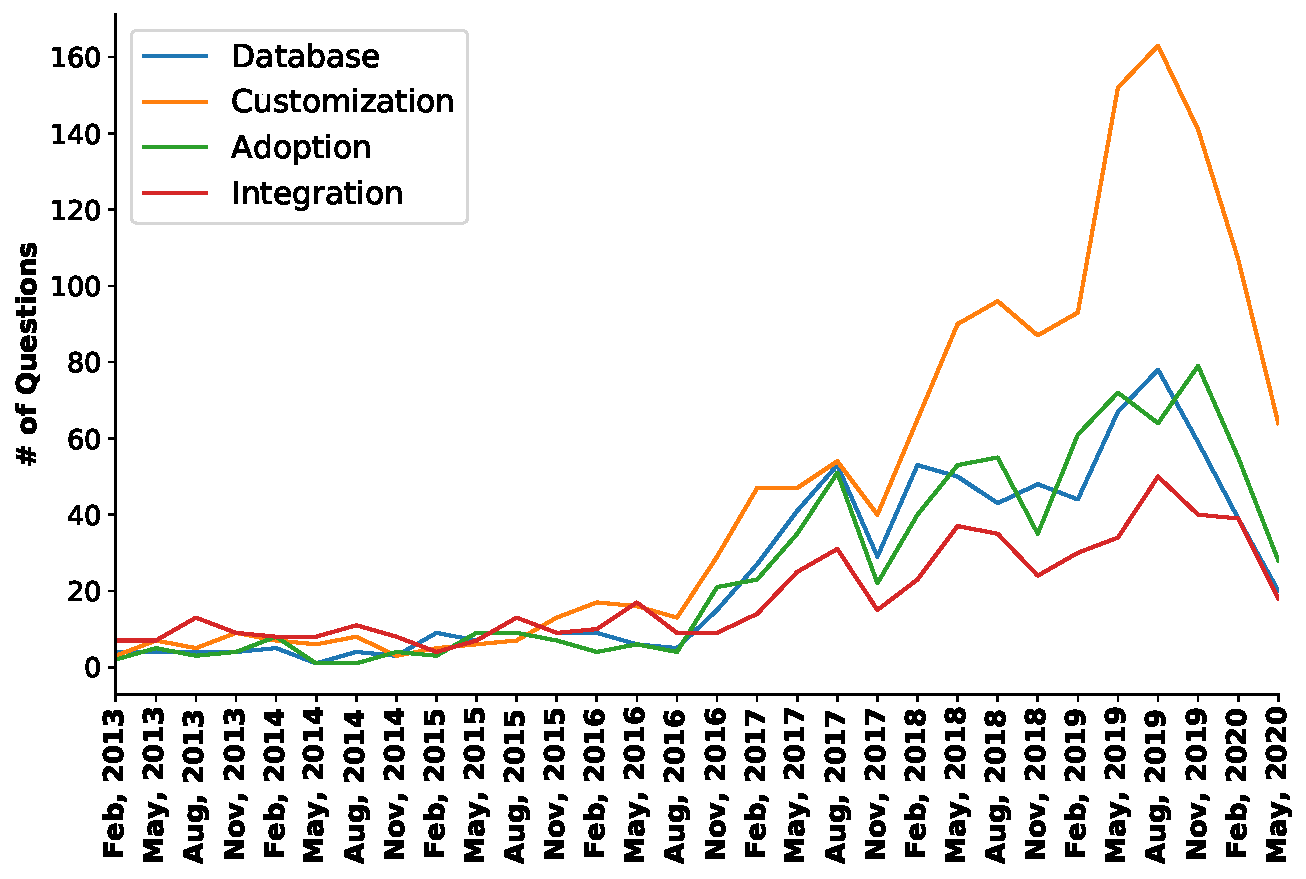
\includegraphics[scale=0.38]{res/Question_per_higher_category_3M.pdf}
% 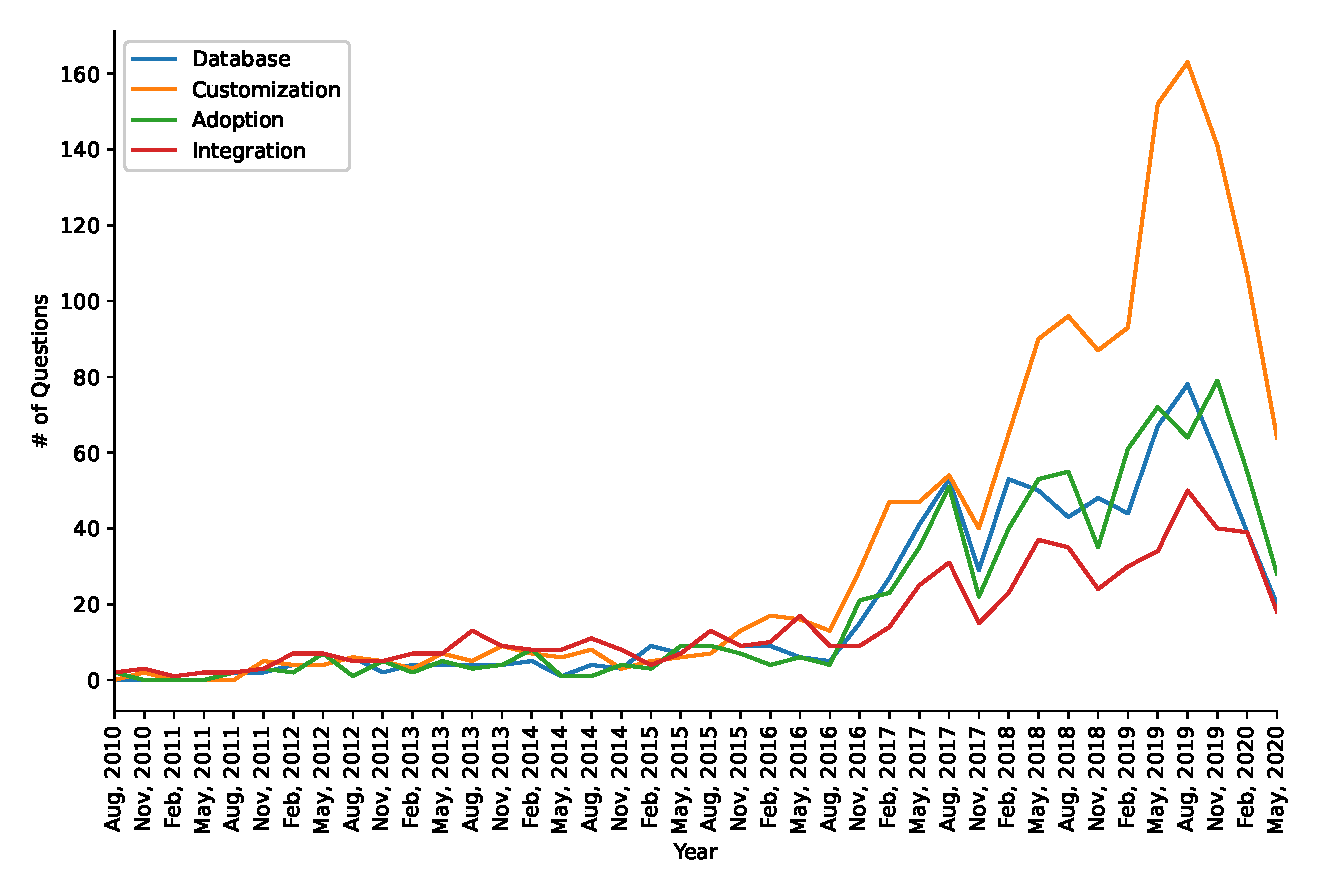
\includegraphics[scale=0.38]{res/Question_per_higher_category.eps}
% 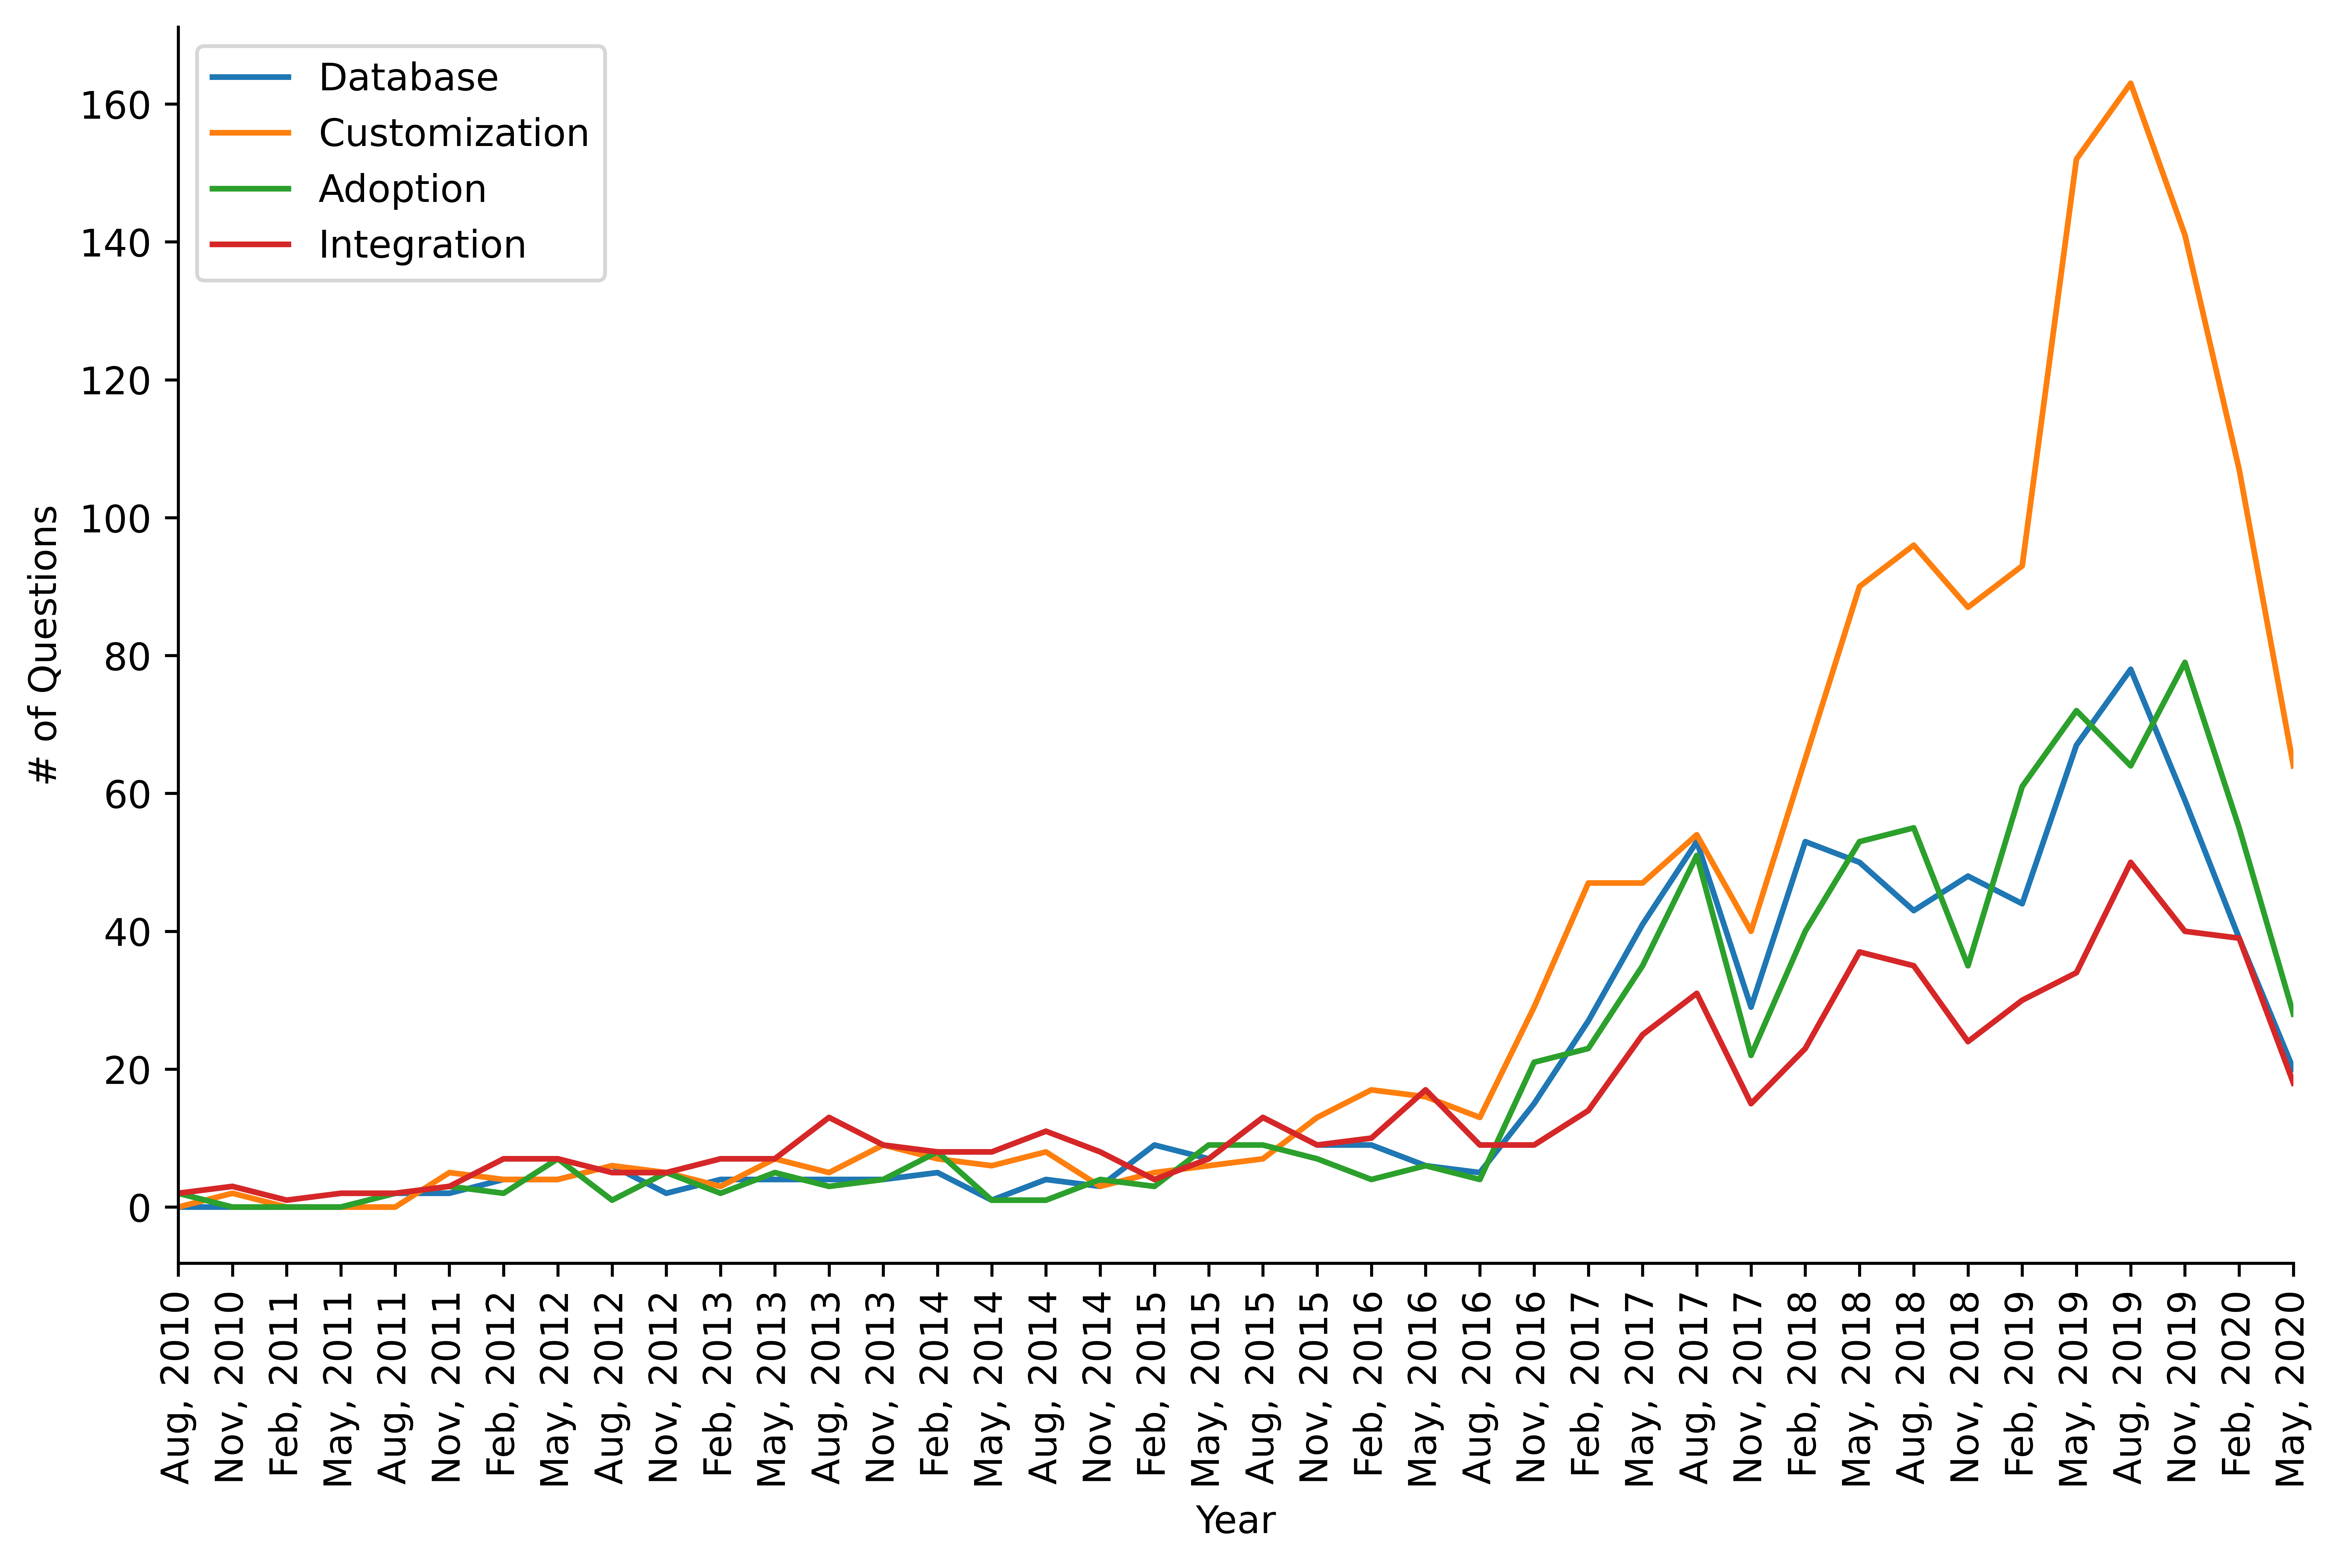
\includegraphics[scale=0.38]{res/Question_per_higher_category.png}
% 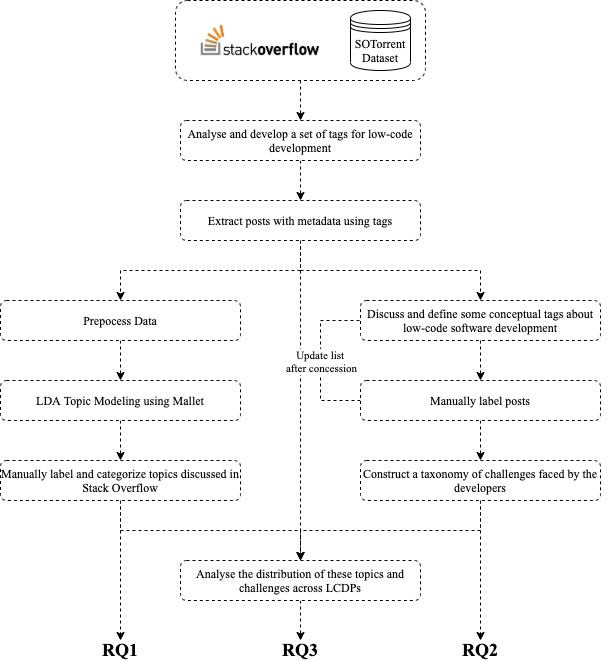
\includegraphics[width=0.35 * linewidth]{res/methology_overview.jpg}
\caption{Low-code topic category evolution over time.}
\label{fig:trend_questions_per_topic_category}
\end{figure}

\begin{figure}[t]
\centering
% 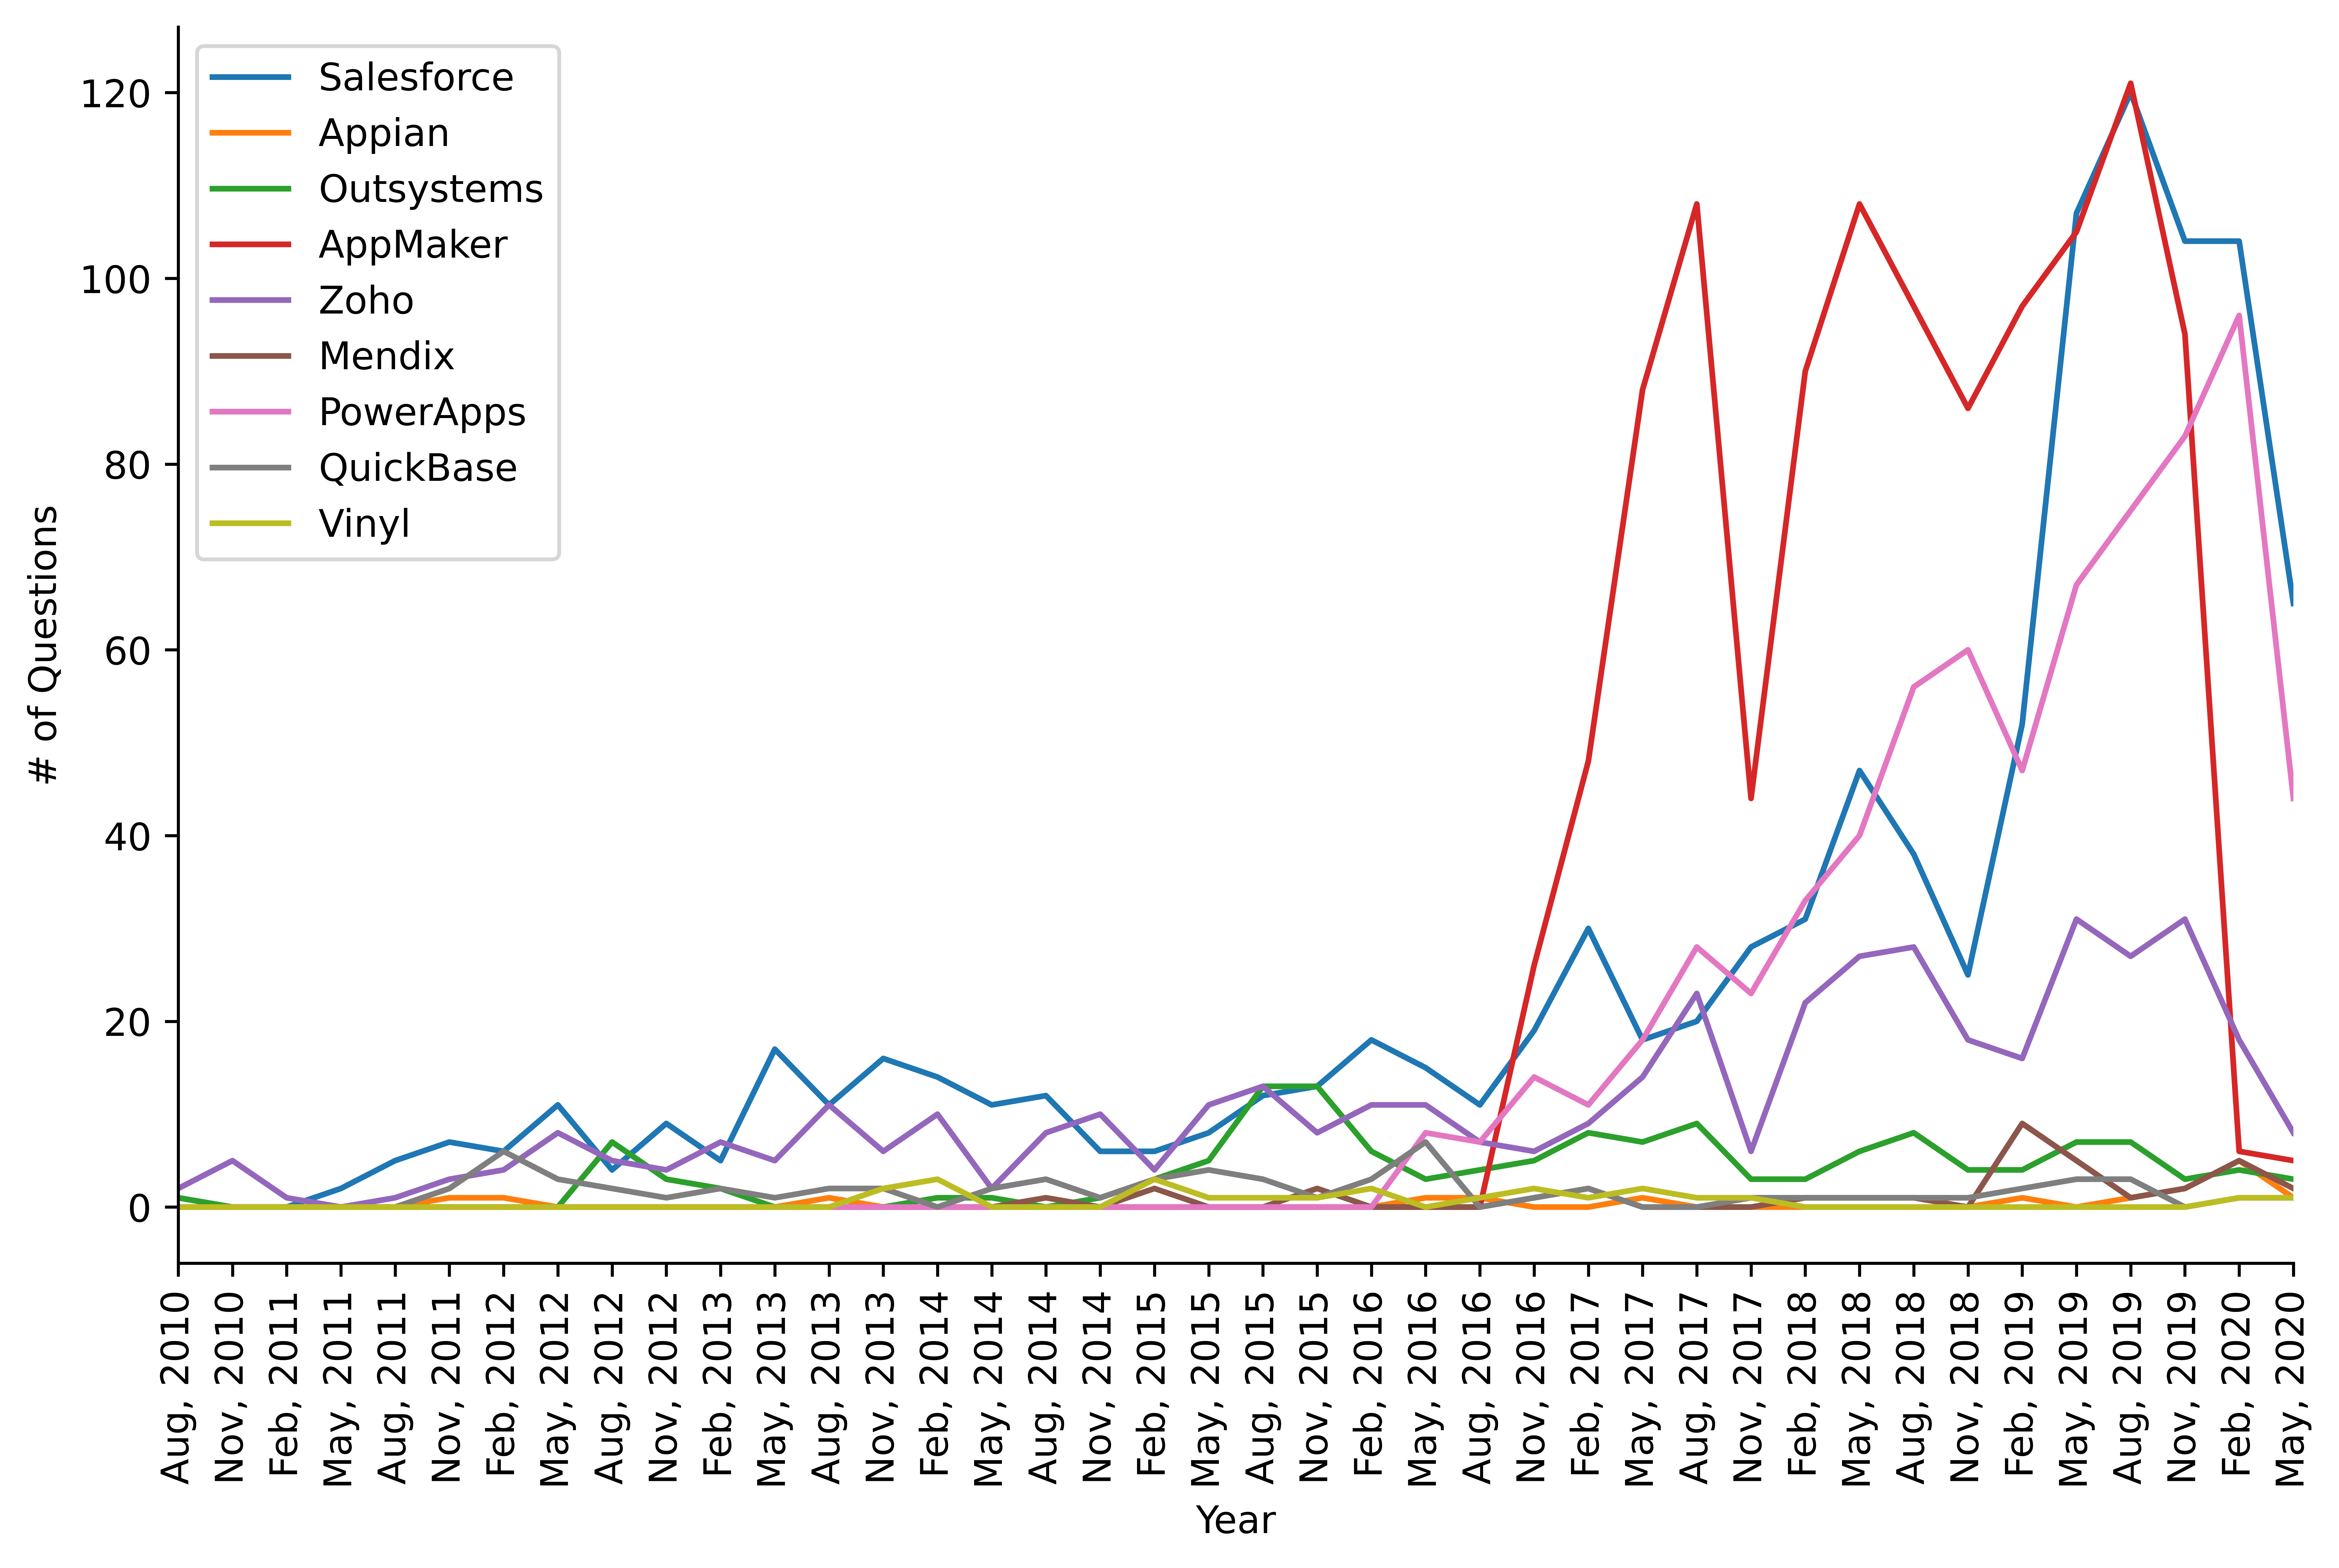
\includegraphics[scale=0.38]{res/question_per_platform.png}
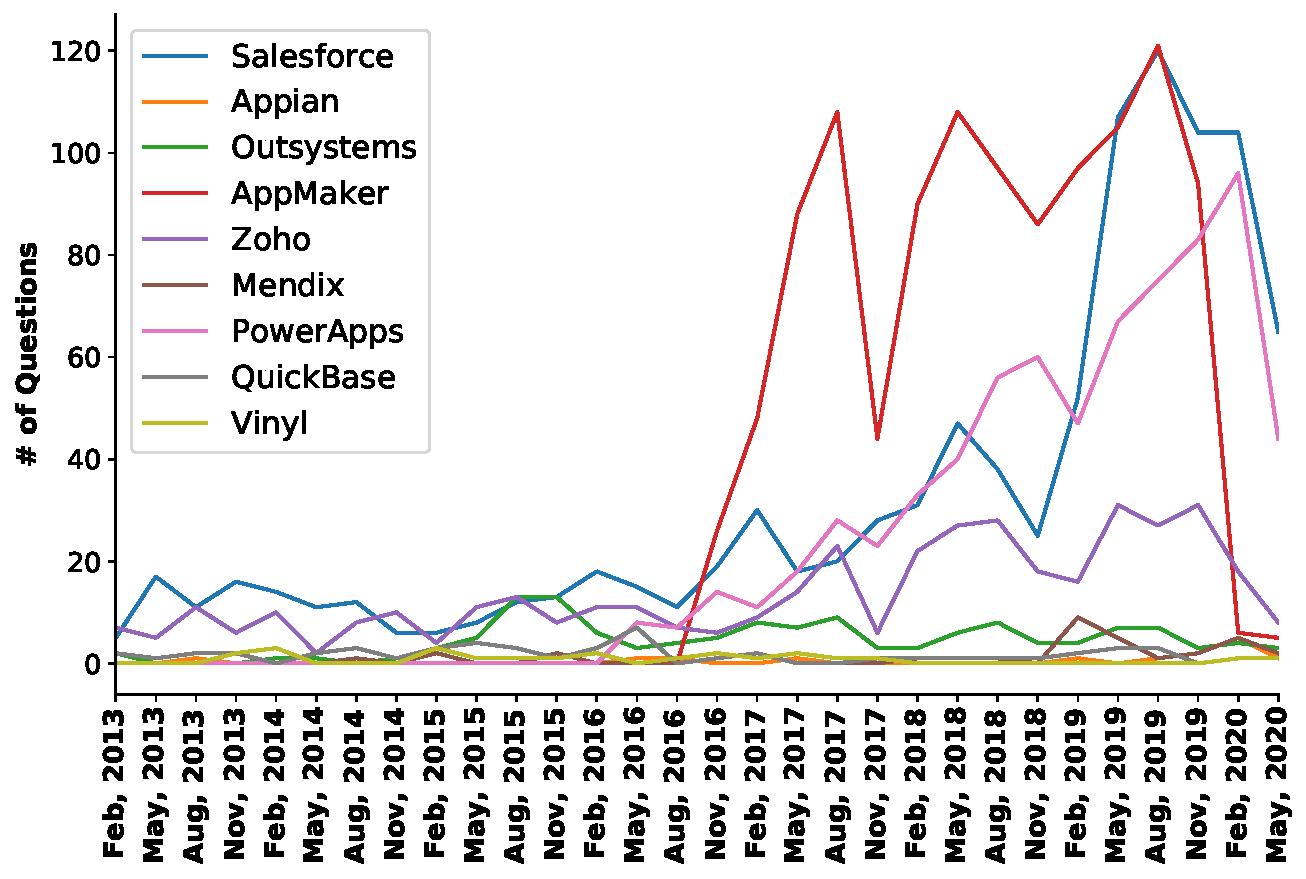
\includegraphics[scale=0.38]{res/question_per_platform_3M.pdf}
\caption{Low-code Platforms evolution over time}
\label{fig:trend_questions_per_platform}
\end{figure}

We further analyze two sudden swings in the number of questions. First, we find an increase of questions in every category after mid-2016, especially for questions about the \textit{Customization} category. Google released App Maker~\cite{googleappmaker} for public use in 2016, which introduced many discussions on LCSD customization. \fig\ref{fig:trend_questions_per_platform}  confirms it and shows a spike in questions about Google App Maker during that time. The second case is that at the beginning of 2020, there is a sharp decline in SO discussions. In Jan 2020, Google announced that they would no longer release new features for Google App Maker and discontinue it by 2021~\cite{google-disc}. It created unrest among the developer community as they were trying to verify this information (\dq{59947680}) and to explore alternatives (e.g., \dq{59985750}). \fig\ref{fig:trend_questions_per_platform} also shows the sudden drop in the number of questions asked about Google App Maker starting Jan 2020.
%Apart from this incident, there has been an overall increasing trend of  LCSD related discussions in SO despite the effect of Global pandemic during the early 2020.

%We also make our dataset publicly available \cite{}. \anindya{It would be an anonymous Git repo link in the footnote, not a citation.} 
%In summary,  LCSD is gaining community attention over time and
%our finding suggests that low-code community tends to pick up new LCSD platforms
%quite positively.


\subsection{Implications of Findings} 

% \gias{Here we will create two charts: (1) A bubble chart like Fig. 4 of Bagerzadeh and Khatchadourian~\cite{Bagherzadeh-BigdataTopic-FSE2019} and (2) the evolution of each challenge type over time by plotting the total number of times each challenge type is found per month. We will use the two charts to discuss the implications of findings}
% % follow Section 4 of \cite{Bagherzadeh-BigdataTopic-FSE2019}

\begin{figure}[t]
%\centering
\vspace{-5mm}
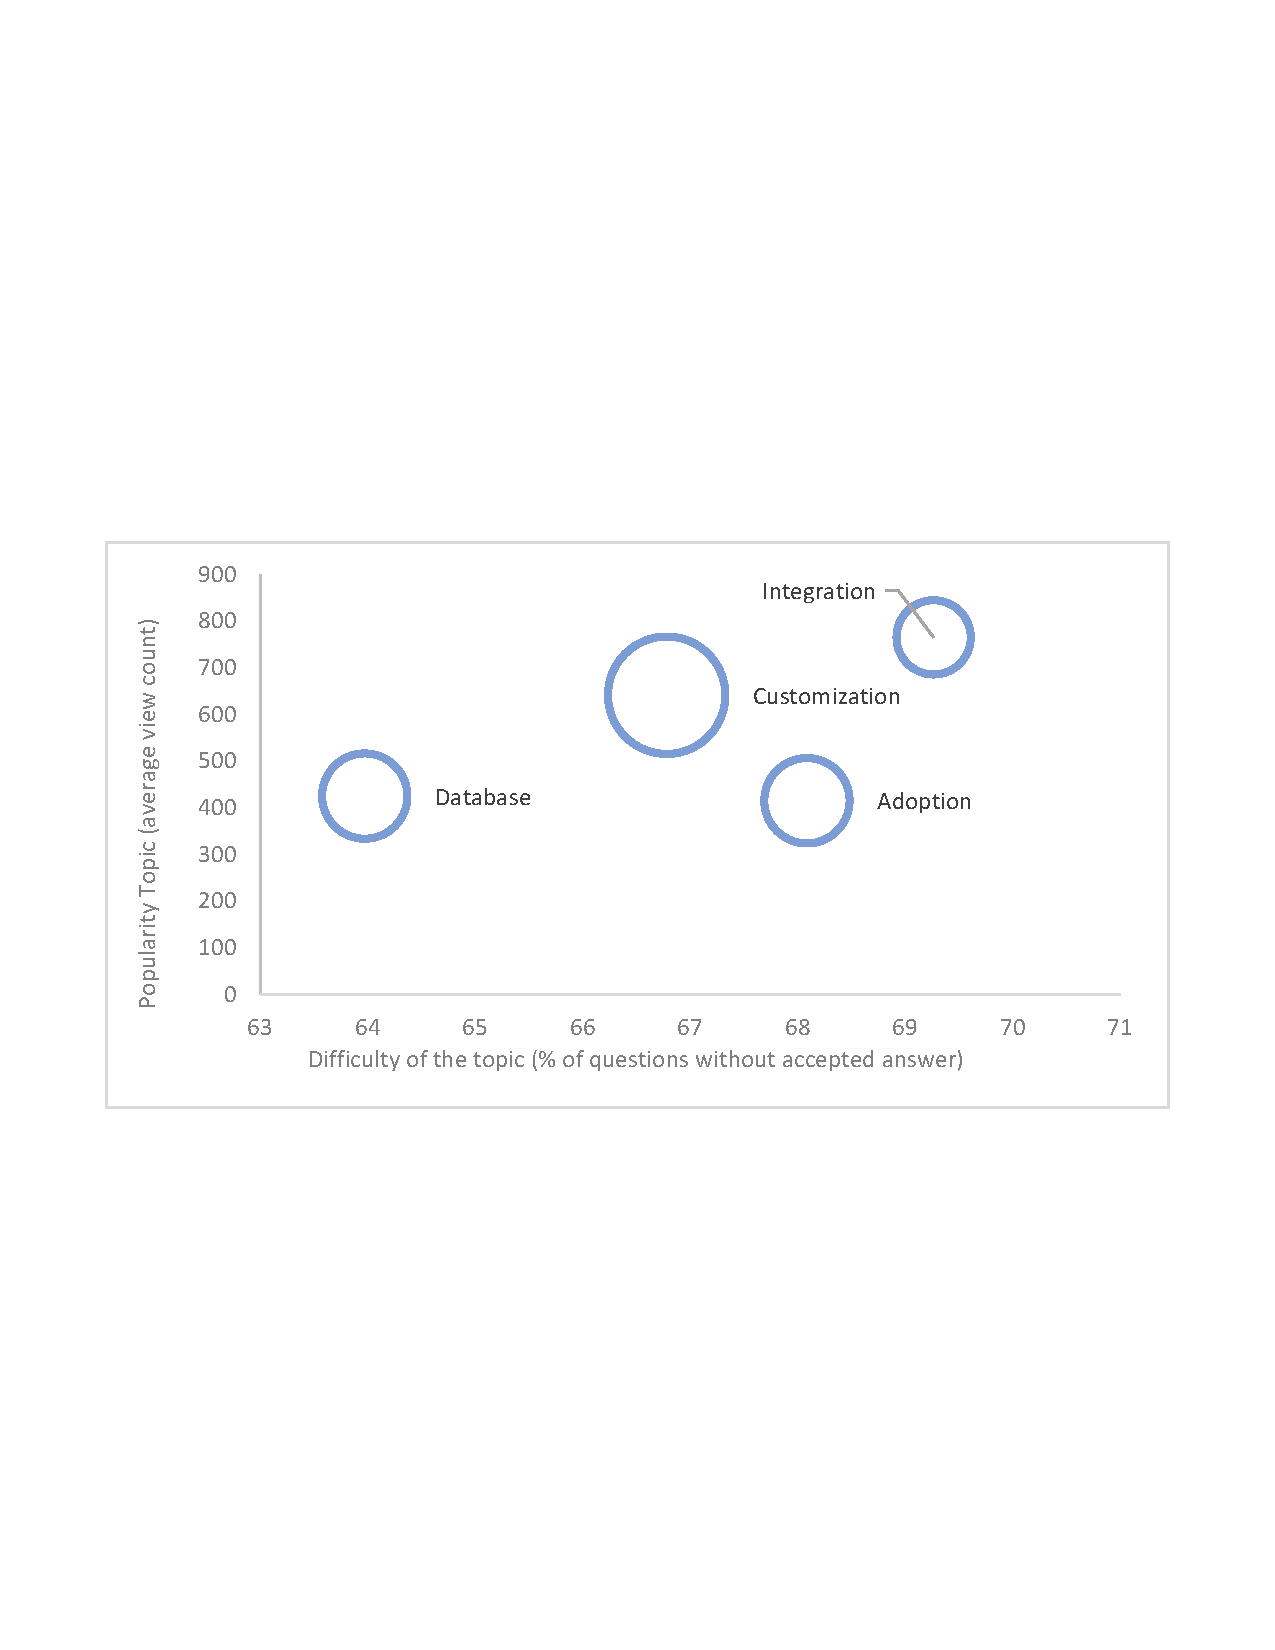
\includegraphics[scale=0.36]{res/popularity_difficulty_bubble_chart.pdf}
\vspace{-15mm}
\caption{Low-code topic categories popularity vs. difficulty}
\label{fig:bubble_diff_pop_per_category}
%\vspace{-5mm}
\end{figure}


% \begin{figure}[t]
% \centering
% 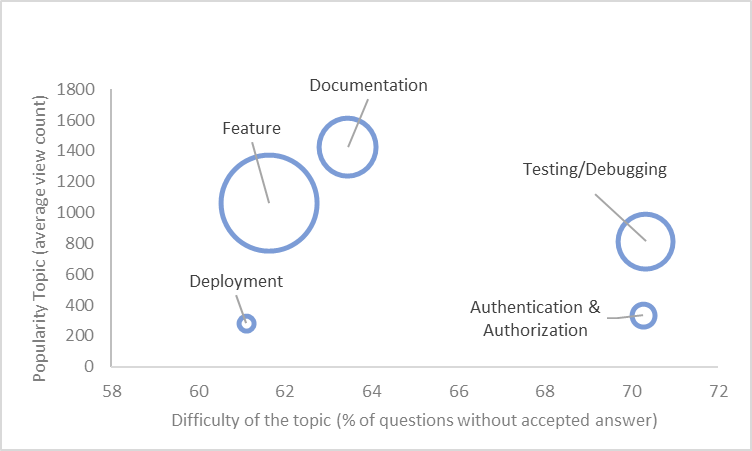
\includegraphics[scale=0.65]{res/bubble_diff_pop_per_challenge.png}
% % 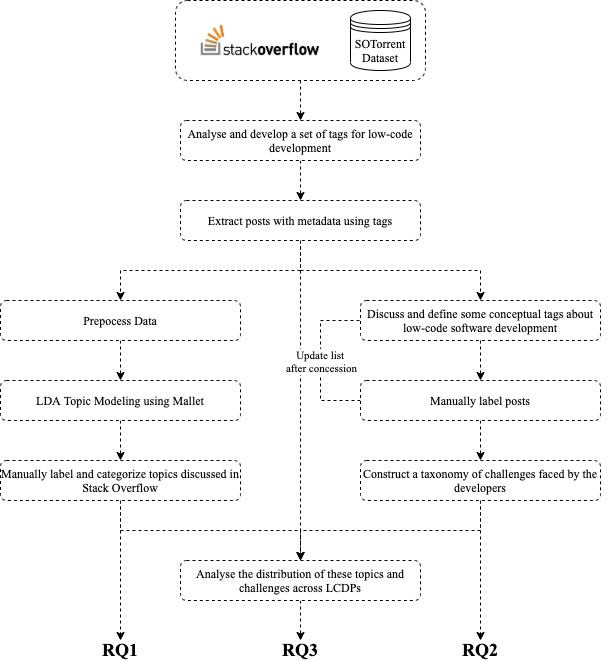
\includegraphics[width=0.35 * linewidth]{res/methology_overview.jpg}
% \caption{Low-code development challenges' popularity vs difficulty}
% \label{fig:bubble_diff_pop_per_challenge}
% \end{figure}

This study can help the low-code community to focus on the pressing issues on the
LCSD paradigm. We discuss the implications of our study findings by stakeholders below.

\bf{\ul{ LCSD Platform Providers.}} 
In order to better understand the issues of LCSD, we present a bubble chart \ref{fig:bubble_diff_pop_per_category} that presents the positions
of low-code categories in terms of popularity vs. difficulty. In this study, we
use the average number of view-count and percentage of questions without accepted
answers as a proxy for the topic category popularity and difficulty,
respectively~\cite{abdellatif2020challenges}. The size of the bubble depends on
the number of questions for that particular topic category.
Figure \ref{fig:bubble_diff_pop_per_category} shows that \textit{Integration} is
the most popular as well as most difficult topic category. On the other hand,
\textit{Database} remains the least difficult category due to the superior database support by  LCSD platforms. As shown in Figure \ref{fig:bubble_diff_pop_per_category},
\textit{Customization} is the largest and prevalent low-code topic category.
Many new practitioners make queries regarding LCSD platforms,
learning resources, basic application and UI customization, and how to get
started with this new emerging technology. We find that \textit{Documentation}
related queries are both very popular and difficult. Our
findings also suggest that many practitioners still face challenges during testing and debugging. Consequently, many of
the questions on this topic remain unanswered. It reveals that to ensure smooth adoption of the LCSD platform, the platform providers should provide better and effective documentation and provide learning resources to reduce entry-level barriers and smooth out the learning curve. 

\textbf{\ul{ LCSD Practitioners/Developers.}} LCSD abstractions and the platform's
feature limitations sometimes make it very difficult to customize and debug. Our
finding shows that the practitioners find third party service \textit{Integration}
and \textit{Platform Feature} category most difficult. It provides valuable
insights for project managers to manage resources better (i.e., human resources and
development time). 
% \anindya{example of integration issue?} 
LCSD platform enables practitioners with diverse experience to contribute to the development process even without a software development
background. However, our finding shows that practitioners find debugging, application
accessibility, and documentation challenging. Hence, the practitioners should take
the necessary steps to understand the tradeoffs LCSD platforms' features deeply. The project manager should adopt specific strategies to learn to customize, debug, and test the application.


\textbf{\ul{ LCSD Researchers \& Educators.}} We find that
the LCSD paradigm's challenges can be different from traditional software development~\cite{sahay2020supporting}. Researchers can focus on the most popular
and difficult topic category \textit{Integration} and
develop a set of metrics to automatically detect documentation quality on
third-party service APIs. Simultaneously, researchers can study how to
provide better tools for practitioners to customize the application.
Security is an open research opportunity for such platforms as a security
vulnerability in such platforms or frameworks could compromise millions of applications and users~\cite{lin2020software}. Researchers can come
up with better testing approaches to ensure faster development and dependability. Educators can also benefit from the results presented in Figure
\ref{fig:bubble_diff_pop_per_category} to prioritize their focus on different topics such as \textit{Database, Customization, and Third-party API Integration}.

% There are many factors that can contribute to the LCSD adoption. Low-code
% researchers, practitioners, platform providers need to consider these factors
% and their trade offs. However, we believe our findings and implications can help
% the decision making process.

% Low-code development platforms has a still long way to go. Practitioners still face difficulty to design UI and application customization and data store. There are lots of research opportunity to improve security, better automatic code generation, server deployment.



% lack of security and scalability discussion

% \paragraph{Community support}
% \paragraph{Community support}
% \paragraph{Documentation/Tutorial support}
% \paragraph{Future software development}

% \paragraph{Training}

% \subsection{Threats to Validity} \label{subsec:validity}
% There are some threats that may affect the validity of our study results. 
% \paragraph{Internal Validity}
% The internal threat refers to the mistakes or errors in our experiments such as missing some related questions regarding low-code development if the questions have not been tagged properly. We double checked to find related tags. There might be some making coding error during LDA topic modelling and SO post extractions. This data extraction have have reviewed by two authors. Our studied X SO posts regarding LCDP. We selected these posts by choosing questions that has at least one tags of some popular LCDP. We have not takes posts that does not have LCDP tags. we reported LDA parameters for replications
% 
% Tags were selected in an open debate session
% difficult to find optimal value of K. We used different values of K and calculated topic coherence score. As LDA is probabilic, we ran our model couple of times and find not significant difference.
% 
% We tried several well known techniques to extract related tags \cite{rosen2016mobile}\cite{bagherzadeh2019going}.
% We tried several well known techniques to manual labelling \cite{bajaj2014mining}\cite{ahmed2018concurrency}.
% We tried several well known techniques to find k \cite{ahmed2018concurrency}\cite{barua2014developers}.
% 
% 
% Only SO might not show the whole picture because due the platform's question's policies, there are some non technical but important challenges such as general soft ware architecture/design questions, comparison between platforms, platform's reputation, support and scalability,
% However large number of  SO questions and community members comments help to mitigate this.
% 
% 
% 
% 
% 
% \paragraph{External Validity}
% 
% Our work does not cover entire low-code ecosystem..
% The external threat to our study can be the generalization that we provided on the challenges that the developers have at different stages of low-code software life cycle. Manual labelling of questions is generally biased but we tried to reduce it taking votes of 4 Authors when there is conflict. After discussion we had around ? percent agreement.
% We have conducted this study by study around ? SO questions and manually reviewing ? questions by four authors. In the future we intend to address this issue by interviewing low-code developers and getting their feedback on our generalization, analysing data from different sources. 
% 
% Further studies should include more data sources.




% \begin{figure}[t]
% \centering
% \hbox{\hspace{-3em}\includegraphics[scale=0.42]{res/questions_per_platform_Per_Two_Month_With_Total.png}}
% % 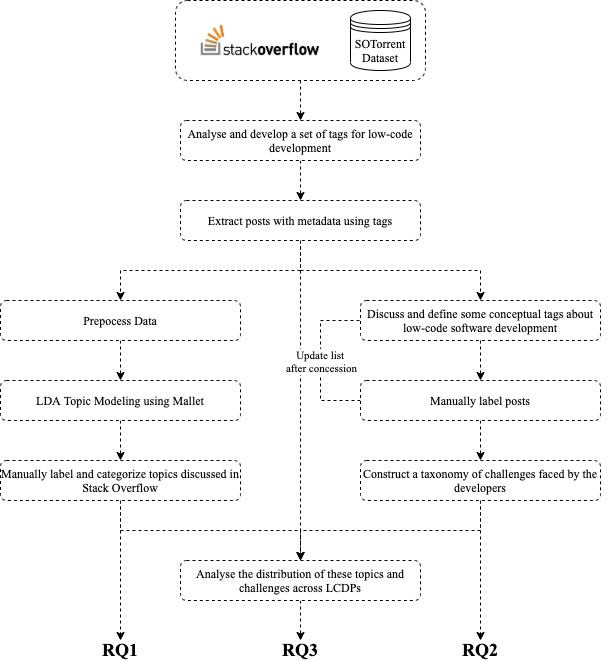
\includegraphics[width=0.35 * linewidth]{res/methology_overview.jpg}
% \caption{Trend of discussions on SO on different low-code development platforms over time}
% \label{fig:questions_trend_per_lcdp_platform}
% \end{figure}
% 
% \begin{table}[htb]
%     \caption{Low-code software development platforms, their popularity, and their significance }
%     \centering
%         \begin{tabular}{|m{5em}|m{10em}|m{2em}|m{3em}|m{3.5em}|}%         
%         \hline
%         \textbf{Platform Name} & \textbf{Tag Name} & \textbf{\# of Posts} & \textbf{Avg view count} & \textbf{Avg favorite count}\\%         
%         \hline
%         \textbf{Salesforce} & salesforce-lightning \newline lwc \newline lightning \newline salesforce-communities \newline salesforce-chatter \newline salesforce-service-cloud \newline aura-framework & 1031 & 619.75	
%  & 1.05 \\%     
%         \hline
%         \textbf{Appian} & appian & 16 &	366.56 &	2  \\%         
%         \hline
%         \textbf{OutSystems} & appian & 147 & 1156.93 & 1.31  \\% 
%         \hline
%         \textbf{AppMaker} & google-app-maker & 1123 & 272.36 & 1.07 \\%         
%         \hline
%         \textbf{Zoho} & appian & 445 & 874.95	& 1.26 \\% 
%         \hline
%         \textbf{Mendix} & mendix & 35 &	459.74 &	1  \\%   
%         \hline
%         \textbf{PowerApps} & powerapps \newline powerapps-formula \newline powerapps-selected-items \newline powerapps-collection \newline powerapps-canvas & 710 &	684.54 & 1  \\% 
%         \hline
%         \textbf{QuickBase} & quickbase & 67 & 575.02 &	0.9  \\% 
%         \hline
%         \textbf{Vinyl} & vinyl & 23	& 289.39	& 1  \\% 
%         \hline
%         \end{tabular}
%     
%     \label{tab:LCDPs_questions_distribution}
% \end{table}
% 
% 
% 
% 
% \begin{figure}[htb]
% \centering
% 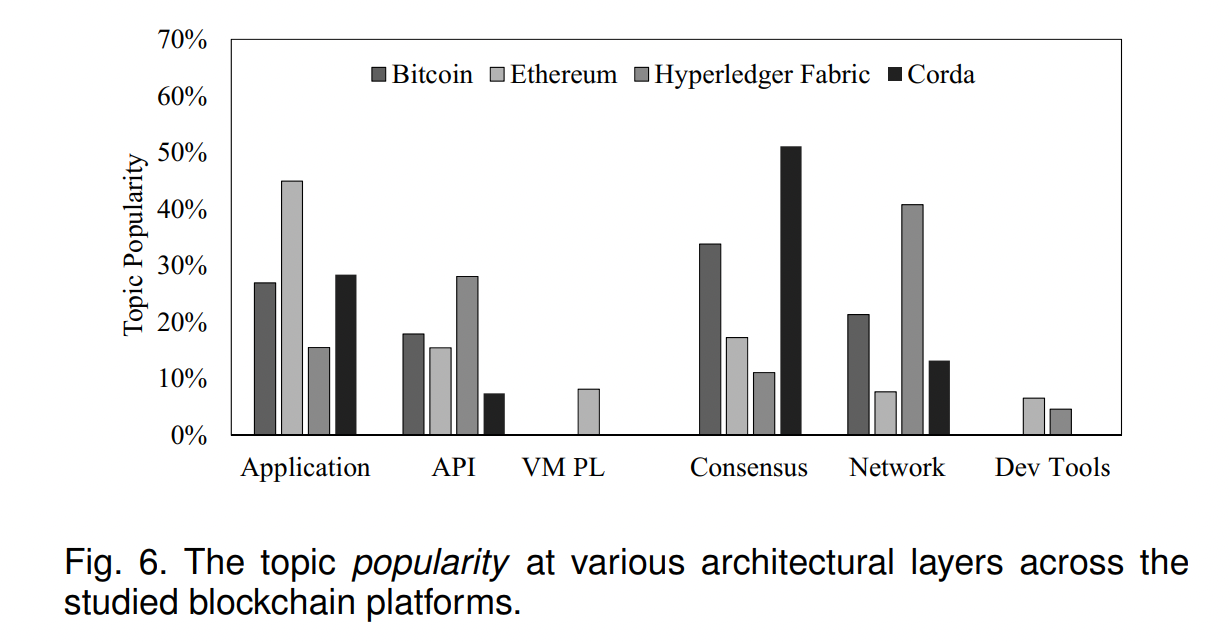
\includegraphics[scale=0.40]{res/bar_block_chain.png}
% % 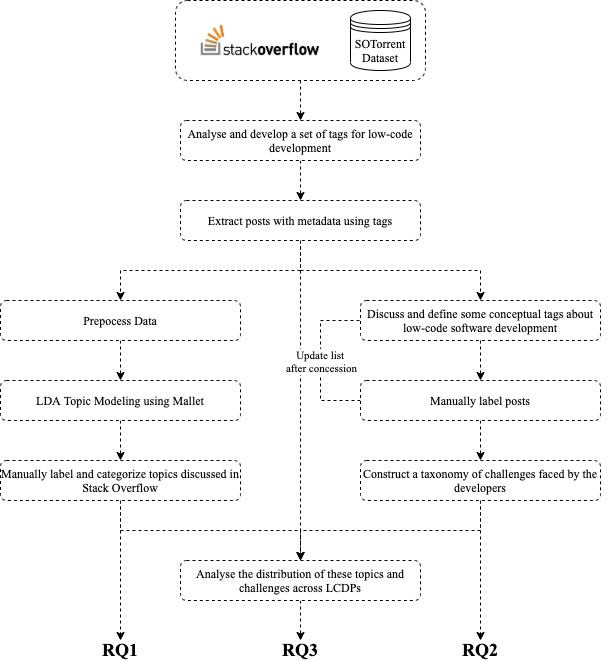
\includegraphics[width=0.35 * linewidth]{res/methology_overview.jpg}
% \caption{(Dummy) How practitioners face challenges in different stages of agile development life cycle in different low-code development platforms over time.}
% \label{fig:challenges_per_lcdp}
% \end{figure}
% 
% \begin{figure}[htb]
% \centering
% 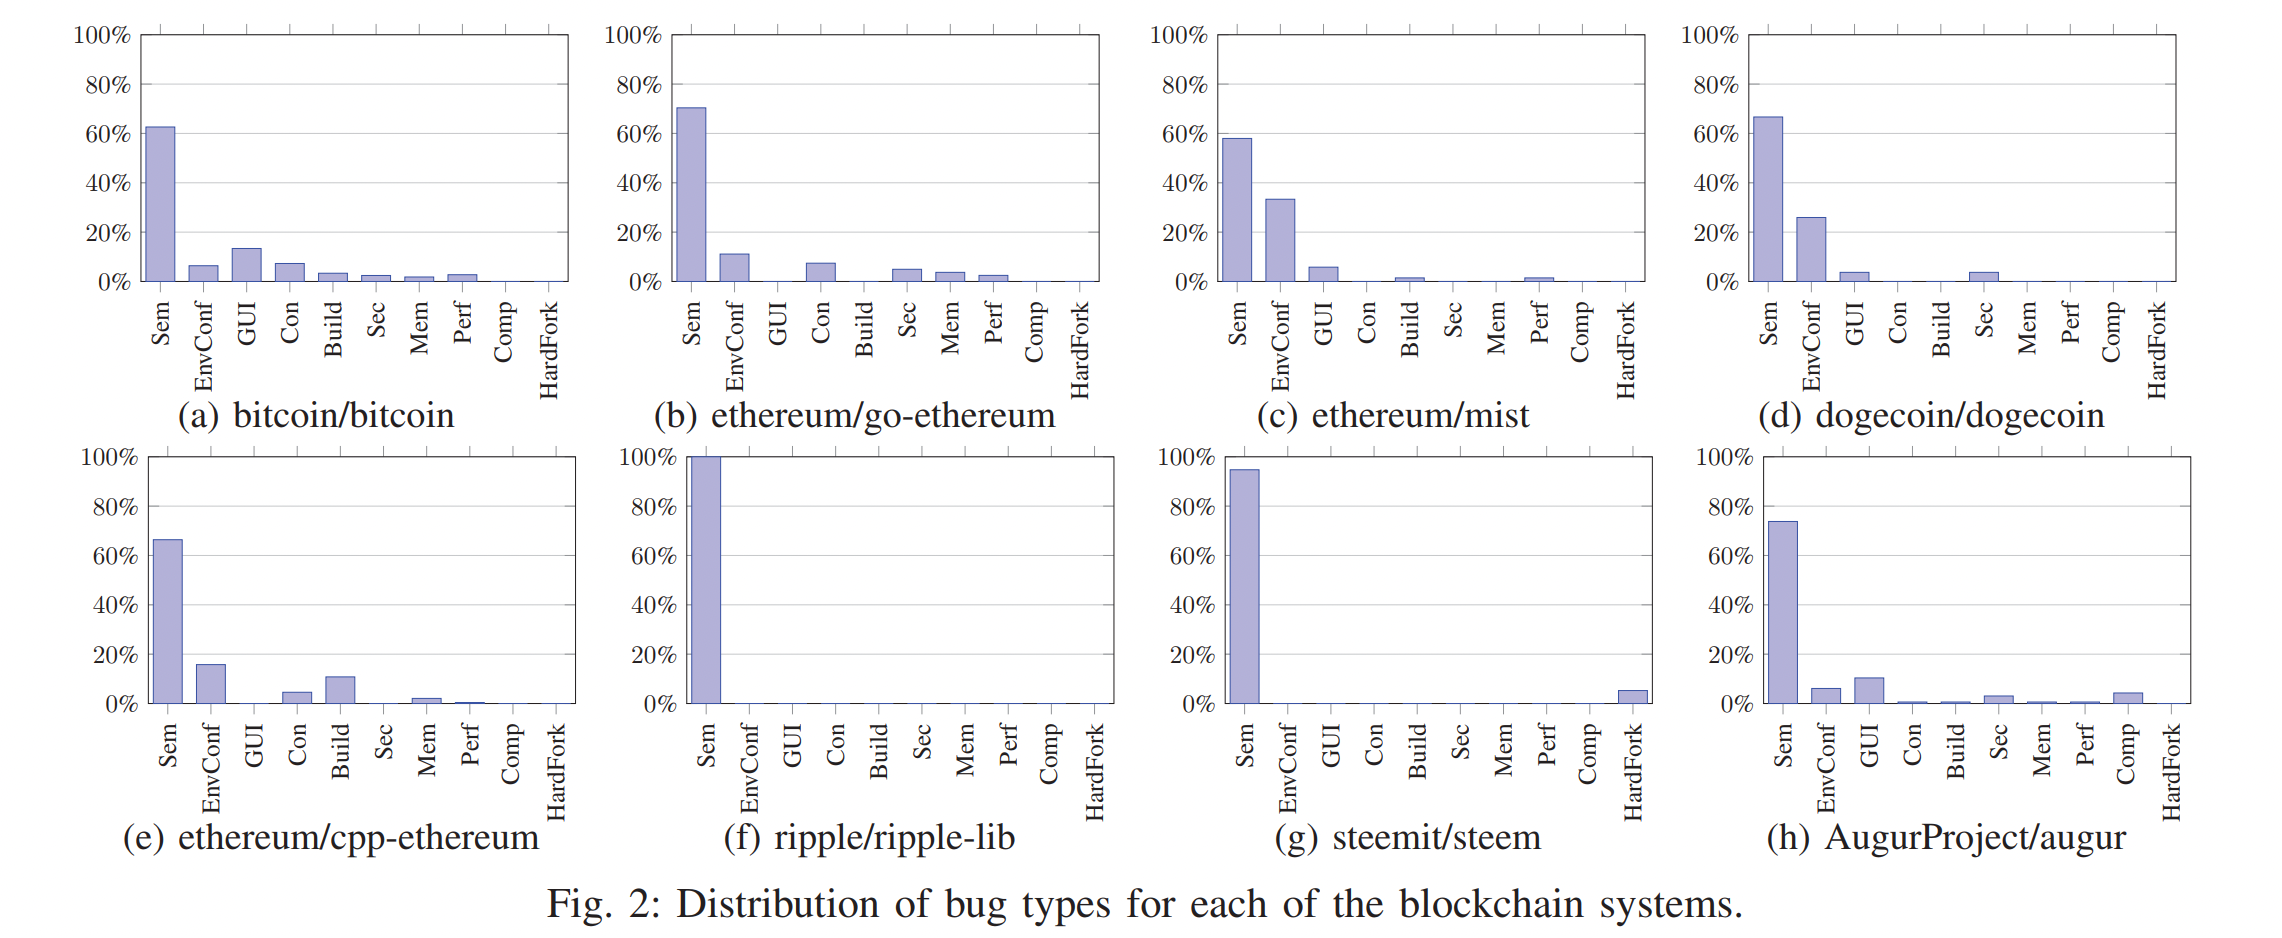
\includegraphics[scale=0.22]{res/bug_accross_platform.png}
% % 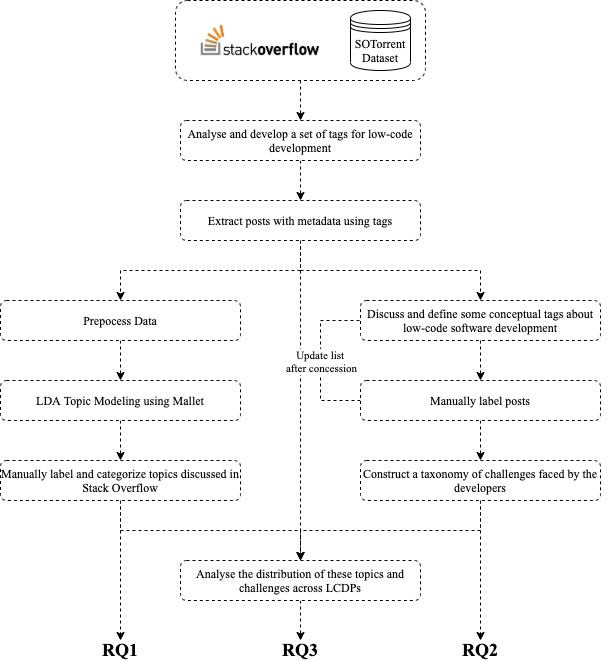
\includegraphics[width=0.35 * linewidth]{res/methology_overview.jpg}
% \caption{(Dummy) How topics are distributed across different low-code development platforms over time.}
% \label{fig:topics_per_lcdp}
% \end{figure}
% 
% 
% 
% 
% \subsubsection{Motivation} 
% % motivate why this research question is important
% Different LCDPs have different set of features, advantages and disadvantages. 
% % For example, Salesforce ? this ? is easier. ? platform provides ? 
% In this research question, we discuss on discussions related to different challenging topics distribute across different low-code development platforms. This will provide valuable insights of about different LCDPs and their usability cases.
% 
% \subsubsection{Approach} 
% % categorize each question+accepted answer by the low code provider tagged or discussed (e.g., zoho, appian, etc.).
% We started with top 9 low-code development platforms (Salesforce, Appian, OutSystems, App Maker, Zoho, Mendix, PowerApps, QuickBase, Vinyl) as presented in Table \ref{tab:LCDPs_questions_distribution}. From our RQ1, we found posts categorized in 5 higher level of topics and from RQ2, we manually labelled ? posts into different technological challenges faced during development. For this research questions we find out how these technical topics and challenges are distributed across different LCDPs.
% 
% % From our manual labeling of questions, and our taxonomy presented \ref{} we showed
% 
% \subsubsection{Results} 
% % report the results
% 
% Table \ref{tab:LCDPs_questions_distribution} shows how many questions are asked about different LCDPs, and popularity and impact. We can see that, in SO the Salesforce(1031) and AppMaker (1157) are the most discussed LCDP and each has more than one thousands of posts. Zoho and PowerApps are second most popular LCDPs, they have around half thousand posts each. Appian, OutSystems, Mendix, QuickBase, Vinyl have around one hundred posts each. Posts in OutSystems have the highest average view count (1157) and Google app maker has the lowest average view count (272). Figure \ref{fig:questions_trend_per_lcdp_platform}  
% and it also shows that total number of discussions on low-code development is increasing over and it also how discussions across different low-code platform are evolving over time.
% 
% Figure \ref{fig:topics_per_lcdp} shows how various topics derived from our topic modeling are distributed across LCDPs. We can see that topic ?, ? and ? is more prevalent in platform ?. Platform ? has the highest number of discussion on ?, ?. ? is also more discussed in platform ?.
% 
% Figure \ref{fig:challenges_per_lcdp} show how different type of challenges are more prevalent across different LCDPs.  We can see ?, ? have more discussion on ?. Discussion related to debugging is more prevalent in ?. In ? there are a lot of posts regarding cloud configuration. ? has quite a few discussion on UI and Application customization. ? has a lot of queries on deployment and user role management.

\section{Threats to Validity}\label{subsec:validity}
% \bf{Internal validity.} This type of threat refers to the mistakes or errors in our
% experiments such as missing some related questions regarding low-code
% development if the questions have not been tagged properly. In order to mitigate this, we examine all the tags that we find in the low-code related questions. Then we use $S_{tag}$ and ${R_tag}$ values to find other tags that are significantly related to our existing low-code tags. This approach and our $S_{tag}$ and ${R_tag}$ values are in line with other related works\cite{chatbot}\cite{ahmed2018concurrency}\cite{rosen2016mobile}\cite{bagherzadeh2019going} that used this measure to find better coverage of a certain SE topic.

% Another potential threat is regarding topic modelling technique where we choice of $K$ = 13 as the optimal number of topics for our dataset $B$. This optimal number of topics have direct impact on the output of LDA. We experimented with different values of $K$ following related works\cite{chatbot}\cite{bagherzadeh2019going}. We used coherence score and manual examination to find the optimal value for $K$ that gives us most relevant and generalized low-code related topics.

% Our manual labelling of questions to agile SDLC phase is another threat to validity. In order to alleviate this each question was labelled by two authors and a third author weighted in in case there were a conflict.

% checked to
% find related tags. There might be some making coding error during LDA topic
% modelling and SO post extractions. This data extraction have have reviewed by
% two authors. Our studied X SO posts regarding LCDP. We selected these posts by
% choosing questions that has at least one tags of some popular LCDP. We have not
% takes posts that does not have LCDP tags. we reported our LDA parameters for
% replications Tags were selected in an open debate session
% difficult to find optimal value of K. We used different values of K and calculated topic coherence score. As LDA is probabilic, we ran our model couple of times and find not significant difference.
% We tried several well known techniques to extract related tags \cite{rosen2016mobile}\cite{bagherzadeh2019going}.
% We tried several well known techniques to manual labelling \cite{bajaj2014mining}\cite{ahmed2018concurrency}.
% We tried several well known techniques to find k \cite{ahmed2018concurrency}\cite{barua2014developers}.
% Only SO might not show the whole picture because due the platform's question's policies, there are some non technical but important challenges such as general soft ware architecture/design questions, comparison between platforms, platform's reputation, support and scalability,
% However large number of  SO questions and community members comments help to mitigate this.

% \bf{External Validity.} This type of threats concern about the generalization of the findings of our study. Our study is based on data from developers discussion on Stack Overflow. However, there are other forums that developer may use to discussion on low-code platform related challenges. But we believe using the data from Stack Overflow provides us the generalizability because Stack Overflow is widely used Q\&A platform for developers from different background. In order to ensure good quality discussion we only used questions with no-negative scores and accepted answers only. However we also believe this study can be improved by including low-code developers' discussions from other forums as well as surveying and interviewing low-code developers about their challenges.

\bf{Internal validity} threats relate to authors'
bias while conducting the analysis. We mitigate the bias in
our manual labeling of topics and  LCSD development phases by consulting the labels among multiple authors. Four of the authors
actively participated in the labeling process. The third author reviewed the final labels and refined the labels by consulting with the first author. \bf{Construct Validity} threats 
relate to the errors that may occur in data collection like the identification of relevant  LCSD tags. To mitigate this, we examine all the tags that we find in the low-code related questions. Then we expanded our tag list using state-of-art approach~\cite{Bagherzadeh-BigdataTopic-FSE2019,abdellatif2020challenges,ahmed2018concurrency, rosen2016mobile}. Another potential threat is the topic modelling technique where we choose $K$ = 13 as the optimal number of topics for our dataset $B$. This optimal number of topics have a direct impact on the output of LDA. We experimented with different values of $K$ following related works\cite{chatbot, bagherzadeh2019going}. We used coherence score and manual examination to find the optimal value for $K$ that gives us the most relevant and generalized low-code related topics. \bf{External Validity} threats relate to the generalizability of our findings. Our study is based on data from developers' discussion on SO. However, there are other forums  LCSD developers may use to discuss. Nevertheless, we believe using SO's data provides us with the generalizability because SO is a widely used Q\&A platform for developers. To ensure good quality discussion, we only use posts with non-negative scores. However, we also believe this study can be complemented by including discussions from other forums, surveying and interviewing low-code developers.


\section{Related Work} \label{sec:related_work}
\nd\bf{Research on low-code development.} LCSD is a relatively new technology, and there are only a few research works in this domain. There is some research on how this emerging technology can be used
in different software applications \cite{lowcodeapp}. Sipio et.
al.\cite{di2020democratizing} presents the benefits and future potential of LCSD
by sharing their experience of building a custom recommendation system in LCSD
platform. Kourouklidis et. al. \cite{kourouklidis2020towards} discusses on
the low-code solution to monitor the performance of the machine learning model. Sahay
et. al. surveys  LCDP and provides a comparison of different LCDPs based on
their useful features and functionalities \cite{sahay2020supporting}. Khorram
et. al.\cite{lowcodetesting} analyses commercial LCSD platforms and present a
list of features and challenges of testing. Ihirwe et. al.~\cite{lowcodeIot}
analyses 16 LCSD platforms and identifies what IoT application-related features and services each platform provides. All these research works
provide a comparison between LCSD platforms and their support on the different type
of applications\cite{alonso2020towards}. To the best of our knowledge, ours is the first empirical study of  LCSD development and platforms based on developer discussions.


\nd\bf{Topic Modeling in Software Engineering.} Our motivation to use topic modeling to understand  LCSD discussions stems from
existing research in software engineering that shows that topics generated from
textual contents can be a good approximation of the underlying
\it{themes}~\cite{Chen-SurveyTopicInSE-EMSE2016,Sun-SoftwareMaintenanceHistoryTopic-CIS2015,Sun-ExploreTopicModelSurvey-SNPD2016}.
Topic models are used recently to understand software
logging~\cite{Li-StudySoftwareLoggingUsingTopic-EMSE2018} and previously for
diverse other tasks, such as concept and feature
location~\cite{Cleary-ConceptLocationTopic-EMSE2009,Poshyvanyk-FeatureLocationTopic-TSE2007},
tracability linking (e.g.,
bug)~\cite{Rao-TraceabilityBugTopic-MSR2011,AsuncionTylor-TopicModelingTraceabilityWithLDA-ICSE2010a},
to understand software and source code history
evolution~\cite{Hu-EvolutionDynamicTopic-SANER2015,Thomas-SoftwareEvolutionUsingTopic-SCP2014,Thomas-EvolutionSourceCodeHistoryTopic-MSR2011},
to facilitate code search by categorizing
software~\cite{Tian-SoftwareCategorizeTopic-MSR2009}, to refactor software code
base~\cite{Bavota-RefactoringTopic-TSE2014}, as well as to explain software
defect~\cite{Chen-SoftwareDefectTopic-MSR2012} and various software maintenance
tasks~\cite{Sun-SoftwareMaintenanceTopic-IST2015,Sun-SoftwareMaintenanceHistoryTopic-CIS2015}.
The SO posts are subject to several studies on various aspects
of software development using topic modeling, such as what developers are
discussing in general~\cite{Barua-StackoverflowTopics-ESE2012}, or about a
particular aspect, e.g., concurrency~\cite{Ahmed-ConcurrencyTopic-ESEM2018}, big
data~\cite{Bagherzadeh2019}, chatbot development~\cite{abdellatifchallenges}.
We are aware of no previous research on understanding
the  LCSD discussions in SO.
% 
% \subsection{Research using data from Stack Overflow}
% 
% Stack Overflow \footnote{\url{https://stackoverflow.com}} is one of the most popular questions and answers website for developers. Developers ask questions on a variety of topics and experts in that area provide solutions. Analysing these discussions can provide valuable insights on what challenges developers and facing and their interest. There has been several studies using stack overflow's data to reveal insights on different aspects of software development technologies analyzing the questions, responses, and relevant metadata \cite{allamanis2013and}, \cite{treude2011programmers}, \cite{wang2013detecting}, \cite{asaduzzaman2013answering}\cite{}, \cite{kuhn2007semantic},  \cite{SOBCSAlahi}, \cite{BlockchainWan},  \cite{chatbot}. Most of these used topic modeling techniques to investigate posts of their interest.
% 
% Allamanis et al.\cite{allamanis2013and} presented how SO questions can be associated with programming concepts. Treude et al. \cite{treude2011programmers} studied on what type of questions are asked in SO and which questions are answered and which are not. Wang et al. \cite{wang2013detecting} presented obstacles in API usage in IOS and Android platform by analysing developers' queries in SO. Asaduzzaman et al.\cite{asaduzzaman2013answering} analysed unanswered questions in Stack Overflow and build a classifier to predict how long a question might take to be answered. Adrian et al. \cite{kuhn2007semantic} used topic modeling on source code to find linguistic topic to find the intention of the code and how these topics are distributed over the system. The security related discussions were comprehensively analyzed by \cite{yang2016security}. Alahi et al. \cite{SOBCSAlahi} conducted a study to understand the primary areas of challenges encountered by the BCS community and Wan et al. \cite{BlockchainWan} also explored the challenges and needs amongst blockchain developers. Abdellatif et al. \cite{chatbot} examined the posts of SO to provide insights on the topics that chatbot developers are interested and the challenges they face. The interest and challenges of concurrency developers were explored by \cite{Ahmed-ConcurrencyTopic-ESEM2018} Ahmed et al. Bagherzadeh and Khatchadourian \cite{Bagherzadeh-BigdataTopic-FSE2019} discussed the insights obtained from big data related posts. Han et al. \cite{han2020DeepLearning} studied both Stack Overflow and Github posts to analyze the discussions about three deep learning frameworks i.e., Tensorflow, PyTorch and Theano.
%  
%  To the best of our knowledge, there is no work that studied low-code related posts using Stack Overflow data. We believe that our study can go a reliable insight on the areas that  are interesting and challenging to the low-code practitioners at an early stage of evolution of low-code.
%  
% 
% % In this Section, we discuss the related studies on LCSD. Then we discuss on the related works that use SO data to study p
% 
% % \subsection{Low-code development}
% % Sahay et. al. surveys  LCDP and provides a comparison of different LCDP's on useful features and functionalities \cite{sahay2020supporting}
% 
% 
% % \subsection{Stack Overflow research}
% % Stack Overflow \footnote{\url{https://stackoverflow.com}} is one of the most popular questions and answers website for developers. Developers ask questions on a variety of topics and experts in that area provide solutions. Analysing these discussions can provide valuable insights on what challenges developers and facing and their interest. There has been several studies using stack overflow's data \cite{}\cite{}\cite{}\cite{}\cite{}.
% 
% 
% % Stack Overflow is widely used by software developers and so it this a good source of information to study developer's' perspective, their challenges. 
% 
% % Using topic modeling Allamanis et al.\cite{allamanis2013and} presented how SO questions can be associted with programming concepts.
% 
% % Treude et al. \cite{treude2011programmers} studied on what type of questions are asked in SO and which questions are answered and which are not. They manually labeled 
% 
% % Wang et al. \cite{wang2013detecting} presented obstacles in API usage in IOS and Android platform by analysing developers' queries in SO.
% 
% 
% % Asaduzzaman et al.\cite{asaduzzaman2013answering} analysed unanswered questions in Stack Overflow and build a classifier to predict how long a question might take to be answered. 
%  
% 
% % \subsection{Topic modeling}
% 
% % Barua et al.\cite{barua2014developers} conducted a studying usin LDA topic modeling to gain insightly information regarding developers community and how topics evolve over time in different software domains.
% %  Rosen et al. \cite{rosen2016mobile} use topic modeling of discussions in Stack Overflow and present popular, difficult topics on mobile development.
%  
% %  Yang et al. use topic modeling with ML algorithm to find popular and difficult security topics and categorized them into 5 topics \cite{yang2016security}
%  
% % Bajaj et al.  \cite{bajaj2014mining} used unsupervised learning to categorize important web development topics, common misconceptions,  and shared and overview of how these questions are evolving over time.
% 
% 
% 
% % Bagherzadeh \& Raffi \cite{bagherzadeh2019going} studied what big data developers asks in SO and their challenges.
% 
% 
% %  Adrian et al. used topic modeling on source code to find linguistic topic to find the intention of the code and how these topics are distributed over the system \cite{kuhn2007semantic}
%  
%  
%  
\section{Conclusions} \label{sec:conclusion}
LCSD is a new paradigm that enables the development of
software applications with minimal hand-coding using visual programming. We present an empirical study that provides insights into the types of topics low-code developers discuss in Stack Overflow (SO). We find 13 low-code topics in our dataset of 4.6K SO posts (question + accepted answers). The posts are collected based on 19 SO tags belonging to the popular nine  LCSD platforms during our analysis. We categorize them into four high-level groups, namely Customization, Platform Adoption, Database, and Integration. Our findings reveal that developers find the external API Integration topic category the most challenging and the Database category least difficult. Dynamic Event Handling is the most popular, as well as the most challenging topic. We find a severe lack of good tutorial based documentation that deters the smooth adaptation of LCSD. We hope that all of these findings will help various  LCSD stakeholders (e.g.,  LCSD platforms, practitioners, SE researchers) to take necessary actions to address the various  LCSD challenges. Since the growth indicates that this technology is likely to be widely adopted by various companies for their internal and customer-facing applications, platform providers should address the prevailing developers' challenges.


%We also manually examined SO discussions and classified the challenges practitioners face during different stages of agile software development life-cycle. We observed that ?, ? is the widely discussed topic in the community and Application development is the most difficult stage of for the practitioners. Many of the practitioners lack general programming and software engineering concepts.  We also presented how topics and challenges are distributed across LCDPs. We found that ? has lots of queries regarding deployment, platform ? has API integration related discussions. 

% Anindya - The above para can be added later if there is space after addressing the ? things







%\bibliographystyle{ACM-Reference-Format}
%\bibliography{sample-bibliography}
\begin{small}
\bibliographystyle{abbrv}
%\bibliography{bibtex}
% \bibliography{consolidated}
\bibliography{consolidated_lc}
\end{small}


\end{document}
